\documentclass[11pt]{article}
\usepackage[a4paper,margin=27mm]{geometry}
\usepackage{microtype}
\usepackage{amsmath,amssymb,amsthm,mathtools}
\usepackage{enumitem,booktabs,array,longtable}
\usepackage{xcolor}
\usepackage{tikz}
\usetikzlibrary{arrows.meta}
\usepackage{hyperref}
\usepackage[capitalise,nameinlink,noabbrev]{cleveref}
\input{glyphtounicode}
\pdfgentounicode=1

\pdfglyphtounicode{parenleftbig}{0028}
\pdfglyphtounicode{parenrightbig}{0029}
\pdfglyphtounicode{parenleftBig}{0028}
\pdfglyphtounicode{parenrightBig}{0029}
\pdfglyphtounicode{parenleftbigg}{0028}
\pdfglyphtounicode{parenrightbigg}{0029}
\pdfglyphtounicode{parenleftBigg}{0028}
\pdfglyphtounicode{parenrightBigg}{0029}
\pdfglyphtounicode{bracketleftbig}{005B}
\pdfglyphtounicode{bracketrightbig}{005D}
\pdfglyphtounicode{bracketleftBig}{005B}
\pdfglyphtounicode{bracketrightBig}{005D}
\pdfglyphtounicode{bracketleftbigg}{005B}
\pdfglyphtounicode{bracketrightbigg}{005D}
\pdfglyphtounicode{floorleftbigg}{230A}
\pdfglyphtounicode{floorrightbigg}{230B}
\pdfglyphtounicode{braceleftbig}{007B}
\pdfglyphtounicode{bracerightbig}{007D}
\pdfglyphtounicode{braceleftBig}{007B}
\pdfglyphtounicode{bracerightBig}{007D}
\pdfglyphtounicode{braceleftbigg}{007B}
\pdfglyphtounicode{bracerightbigg}{007D}
\pdfglyphtounicode{braceleftBigg}{007B}
\pdfglyphtounicode{bracerightBigg}{007D}

\pdfglyphtounicode{summationtext}{2211}
\pdfglyphtounicode{summationdisplay}{2211}
\pdfglyphtounicode{producttext}{220F}
\pdfglyphtounicode{productdisplay}{220F}
\pdfglyphtounicode{integraltext}{222B}
\pdfglyphtounicode{integraldisplay}{222B}
\pdfglyphtounicode{uniondisplay}{22C3}
\pdfglyphtounicode{intersectiondisplay}{22C2}
\pdfglyphtounicode{radicalbig}{221A}
\pdfglyphtounicode{radicalBig}{221A}
\pdfglyphtounicode{hatwide}{0302}

\pdfglyphtounicode{parenlefttp}{239B}
\pdfglyphtounicode{parenleftbt}{239D}
\pdfglyphtounicode{parenrighttp}{239E}
\pdfglyphtounicode{parenrightbt}{23A0}
\pdfglyphtounicode{bracketlefttp}{23A1}
\pdfglyphtounicode{bracketleftbt}{23A3}
\pdfglyphtounicode{bracketrighttp}{23A4}
\pdfglyphtounicode{bracketrightbt}{23A6}
\pdfglyphtounicode{bracelefttp}{23A7}
\pdfglyphtounicode{braceleftmid}{23A8}
\pdfglyphtounicode{braceleftbt}{23A9}
\pdfglyphtounicode{braceex}{23AA}
\pdfglyphtounicode{vextendsingle}{23D0}
\pdfglyphtounicode{vextenddouble}{2016}

\pdfglyphtounicode{mapsto}{007C}

\usepackage{accsupp}
\let\AstraOriginalMapsto\mapsto
\let\AstraOriginalLongmapsto\longmapsto
\let\AstraOriginalLongrightarrow\longrightarrow
\renewcommand{\mapsto}{\mathrel{%
  \BeginAccSupp{method=hex,unicode,ActualText=21A6}%
  \AstraOriginalMapsto
  \EndAccSupp{}}}
\renewcommand{\longmapsto}{\mathrel{%
  \BeginAccSupp{method=hex,unicode,ActualText=27FC}%
  \begingroup
    \let\mapsto\AstraOriginalMapsto
    \let\longrightarrow\AstraOriginalLongrightarrow
    \AstraOriginalLongmapsto
  \endgroup
  \EndAccSupp{}}}


\pdfglyphtounicode{suppress}{002F}
\let\AstraOriginalLStroke\l
\DeclareRobustCommand{\l}{%
  \BeginAccSupp{method=hex,unicode,ActualText=0142}%
  \AstraOriginalLStroke
  \EndAccSupp{}}

\pdfinfoomitdate=1
\pdftrailerid{}
\pdfsuppressptexinfo=15
\hypersetup{colorlinks=true,linkcolor=blue!45!black,citecolor=green!35!black,
  urlcolor=blue!45!black,pdftitle={Almost-everywhere regularity of stationary integral varifolds},
  pdfauthor={OpenAI},pdfsubject={Geometric measure theory and minimal submanifolds}}
\newcommand{\R}{\mathbb R}
\newcommand{\N}{\mathbb N}
\newcommand{\HH}{\mathcal H}
\newcommand{\eps}{\varepsilon}
\newcommand{\dd}{\mathop{}\!d}
\DeclareMathOperator{\spt}{spt}
\DeclareMathOperator{\supp}{supp}
\DeclareMathOperator{\dist}{dist}
\DeclareMathOperator{\Lip}{Lip}
\DeclareMathOperator{\tr}{tr}
\DeclareMathOperator{\Div}{div}
\DeclareMathOperator{\vol}{vol}
\DeclareMathOperator{\osc}{osc}
\newtheorem{theorem}{Theorem}[section]
\newtheorem{lemma}[theorem]{Lemma}
\newtheorem{proposition}[theorem]{Proposition}
\newtheorem{corollary}[theorem]{Corollary}
\newtheorem{claim}[theorem]{Claim}
\theoremstyle{definition}
\newtheorem{definition}[theorem]{Definition}
\newtheorem{remark}[theorem]{Remark}
\numberwithin{equation}{section}
\setlist{topsep=4pt,itemsep=2pt,parsep=0pt}
\setlength{\emergencystretch}{1.5em}
\title{Almost-everywhere regularity of stationary integral varifolds}
\author{OpenAI}
\date{September 23, 2026}
\begin{document}
\maketitle
\begin{abstract}
We resolve the almost-everywhere regularity conjecture of Brena, Decio, and
De Lellis for stationary integral varifolds of arbitrary positive dimension
and codimension in Euclidean open sets. The singular set has zero measure in
the dimension of the varifold: near almost every support point, the varifold
is a constant positive integer multiple of a smooth embedded minimal
submanifold. The corresponding statement also holds on round spheres.
\end{abstract}
\begingroup
\small
\tableofcontents
\endgroup
\clearpage
\section{Introduction}\label{sec:introduction}

A stationary integral varifold is a measure-theoretic minimal surface with
integer multiplicity. Its tangent plane exists almost everywhere, but a tangent
plane alone need not describe an entire neighborhood. The basic regularity
question is whether the points without a smooth minimal neighborhood can carry
positive measure. We prove that they have zero $m$-dimensional measure.

Let $m,n\geq1$, let $U\subset\R^{m+n}$ be open, and let $E\subset U$ be
countably $m$-rectifiable. Let $\theta:E\to\N\setminus\{0\}$ be measurable and
locally integrable with respect to $\HH^m$. Write
\[
 \mu(A)=\int_{E\cap A}\theta\,\dd\HH^m,
 \qquad P(x)=P_{T_xE}.
\]
The associated integral varifold $V$ is stationary if
\begin{equation}\label{eq:stationarity}
 \int \tr(P(x)DX(x))\,\dd\mu(x)=0
 \quad\text{for every }X\in C_c^1(U;\R^{m+n}).
\end{equation}
A point $p\in\spt\mu\cap U$ is \emph{regular} if there are a neighborhood
$W$ of $p$, a smooth embedded minimal $m$-submanifold $\Sigma\subset W$, and
an integer $q\geq1$ such that the restriction of the varifold to $W$ is
$q|\Sigma|$. The remaining support points form $\operatorname{Sing}V$.

\begin{theorem}\label{thm:main}
Every stationary integral $m$-varifold in an open subset of $\R^{m+n}$ satisfies
\[
 \HH^m(\operatorname{Sing}V)=0.
\]
Here $m,n\geq1$ are arbitrary. No stability, minimizing, orientability,
density upper bound, or codimension-one hypothesis is required.
\end{theorem}

\begin{corollary}[Round spheres]\label{cor:round-spheres}
Let $m,n\geq1$ and let $V$ be an integral $m$-varifold on the full unit round
sphere $S^{m+n}$, stationary for variations tangent to the sphere. A support
point is regular if on a spherical neighborhood $V=q|\Sigma|$ for an integer
$q\geq1$ and a smooth embedded minimal $m$-submanifold $\Sigma$ of the sphere.
If $\operatorname{Sing}_S V$ denotes the remaining support points, then
\[
 \HH^m_{g_{\mathrm{round}}}(\operatorname{Sing}_S V)=0.
\]
No fixed upper bound on mass, density, or multiplicity is required, nor are
stability, orientability, or mod-two cyclicity. The same conclusion holds on
every round sphere of positive radius.
\end{corollary}

\Cref{sec:spheres} derives this corollary from \Cref{thm:main} by a
separate cone argument. That proof adapts the hypersurface first-variation
calculation in \cite[Lemma~6.1]{OpenAISolomonYau2026} and rederives it in
the present dimensions.

\subsection{Background and significance}

Allard's regularity theory gives a relatively open dense regular set and, in
particular, regularity at density-one points \cite{Allard1972}; see also
\cite[Theorem~23]{Allard1987} and
\cite[Chapter~5, Theorem~6.1 and Corollary~6.3]{Simon2018}. Higher integer
density presents a different issue: dividing a varifold by its density at a
point need not preserve the almost-everywhere lower density bound required by
that theorem in a neighborhood. Standard accounts of the first variation,
monotonicity, and integral varifolds may be found in \cite{Simon1983}.

Simon's 2018 notes already record the question whether the singular set
must be $\HH^m$-null even when the generalized mean curvature is zero
\cite[Chapter~5, Remark~6.4]{Simon2018}. The measure-zero singular-set
assertion is Conjecture~1.2 of Brena, Decio,
and De Lellis~\cite{BDD2025}. \Cref{thm:main} proves this conjecture in its
full Euclidean scope. They isolate a local criterion in Conjecture~1.3:
a support point with a unique tangent varifold $Q|\Pi|$, where $\Pi$ is an
$m$-plane and $Q$ a positive integer, should be regular when the mass of
$\{\theta\ne Q\}$ in a ball of radius $r$ about it is $o(r^m)$.
They then propose approximating the varifold by a smooth minimal graph
with the squared-height integral vanishing to every order, followed by a
unique-continuation step that upgrades this contact to local support containment
\cite[Conjectures~1.3--1.5]{BDD2025}. Their analysis of multiplicity and
height in flat cylinders also provides useful precedents for the local
estimates developed here \cite[Theorem~1.9 and Lemma~2.3]{BDD2025}.

Related progress concerns the differentiability of a countable covering.
Menne proved second-order rectifiability for integral varifolds of
locally bounded first variation \cite[Theorem~3.6]{Menne2013}. For stationary
integral varifolds of dimension at least two, Brena, De Lellis, and
Franceschini proved smooth rectifiability and infinite-order approximation
at $\mu$-almost every point by one smooth graph
\cite[Theorems~1.2 and~1.3]{BDLF2025}. The approximating graph in the latter
statement is not asserted to be minimal; Brena--Decio--De Lellis present
this as a weaker form of their approximation conjecture
\cite[Theorem~1.8]{BDD2025}. Kolasi\'nski obtains rectifiability of every
finite order and an alternative proof of the smooth-rectifiability
conclusion, following an architecture he credits to Menne
\cite[Theorem~1.1, Corollary~10.8, and the historical note in Section~1]
{Kolasinski2026}.
Smooth rectifiability gives a countable smooth covering outside a
$\mu$-null set; \Cref{thm:main} requires equality with one smooth minimal
submanifold throughout a neighborhood of almost every point.

In codimension one, Hirsch and Spolaor prove almost-everywhere regularity
for integral currents that are stationary as varifolds and have density
at most two at every support point \cite[Theorem~1.1]{HS2025}.
These current and multiplicity hypotheses distinguish that result from
the arbitrary-codimension statement here.

De Lellis, Hirsch, Lihn, and Spolaor construct, in a smooth Riemannian
metric, a stationary varifold with a double-plane tangent at an exceptional
point and topology accumulating there \cite[Theorem~1.1]{DLHLS2026}.\footnote{In
their respective disclosures, Kolasi\'nski reports using Claude AI and
Claude Code, mostly Opus~5; the abstract of De Lellis--Hirsch--Lihn--Spolaor
credits a crucial suggestion to \texttt{gpt-astra-6}. These attributions
follow the cited papers' own descriptions.}

\subsection{The argument}

The main estimate compares projected mass and tilt with their leading terms
kept signed. In product coordinates $\R^m\times\R^n$, let $\pi$ be
projection onto the first factor, fix a positive integer $Q$, and let
$P_{vv}$ be the vertical block of the tangent projection. With lengths
and mass normalized to the working radius, define
\[
 M=\pi_\#\mu-Q\,\dd y,
 \qquad D=\pi_\#(\tr P_{vv}\,\mu).
\]
Here $|M|$ denotes the total variation of the signed measure $M$, and
$\tau=|M|+D$ is the positive excess measure in this flat setting.
When $\tau$ has mass at most $d$ on a fixed enlarged ball, we prove an
interior bound of the form
\begin{equation}\label{eq:intro-signed}
 \int w(2M-D)
 \leq d\exp\!\left[-F_Q\!\left(\log\frac1d\right)\right]
\end{equation}
for nonnegative Lipschitz weights with fixed bounds. The explicit function
$F_Q$ grows faster than every fixed power of $\log T$ as $T\to\infty$.
\Cref{sx:signed} gives the precise statement, including the curvature error
for a reference surface of sufficiently high finite regularity. Retaining the sign permits a substantially
smaller error than an absolute-value estimate.

The proof of \eqref{eq:intro-signed} is an induction on $Q$. A
heat-potential construction turns a positive violation into a positive
measure on selected centers and scales. At each selected point it gives
an initial sign and a nonnegative cumulative integral along larger scales;
the selection includes vertical sides of the stopping boundary. For
configurations whose normal heights separate into groups, a stopping
argument reduces the estimate to stationary restrictions with smaller
integer counts. The resulting comparison controls tilt away from the groups.

Along a selected path, we take a supremum of damped signed-mass averages
over larger scales and compare it with a clipped squared-distance moment
from an unordered list of at most $Q$ representative normal heights.
A weighted combination of this moment and the cumulative contact integral
stays below the supremum even when representative heights merge. On an
interval without a merger, this comparison forces a quantitative amount
of tilt at many scales. Normal stationarity turns that tilt into a flux
pairing height displacement with radial tilt. A higher height moment
prevents all of that flux from concentrating on sets that have small base
volume but large local excess density. At each selected scale this yields
a base cube in which a quantitative fraction of the $\tau$-mass remains
below a density threshold at all smaller dyadic scales. Packing these
nested cubes shows that the union of their full innermost members has small
$\tau$-mass. A final charge bounds the contact measure by the mass of that
union, contradicting the original violation.

For regularity, fix a point where dilated varifolds converge to a
multiplicity-$Q$ plane
and the mass of other multiplicities has relative density zero. At each
nearby base point, we fit minimal graphs at successive scales, stopping
when a prescribed bound on the support height fails. The correction of
each fit is closely related
to the Jacobi regularization and nonlinear correction of
Brena--De Lellis--Franceschini \cite[Sections~2 and~6]{BDLF2025}.
A centered first-moment estimate, combined with elliptic regularity,
makes neighboring fits agree to second order in their height error.
The signed estimate is first used in a contradiction argument for a
sequence of failed fits normalized by their height errors. Together with
the limiting first-variation identities, its one-sided
inequality shows that the limiting squared-height measure is nonzero in
every interior subball. Strong control of the centered first moment,
together with the integer count $Q$, then forces that second moment to
come from separated projection entries of lower multiplicity on a definite
portion of each such ball. The regions
influenced by failures therefore have vanishing relative volume.

The compatible fits can now be glued into one fixed center of sufficiently
high finite regularity. The weighted integral of the squared mean curvature
and the square of its first derivative is bounded by the corresponding
squared-height integral. The support height is zero outside the regions
influenced by failures. Almgren developed the center-manifold approach
to higher-multiplicity regularity \cite{Almgren2000};
De Lellis--Spadaro construct their center by gluing smoothed local averages
\cite{DLS2016II}. For the inward step we use the comparison of height and
energy in the frequency method of this program
\cite[Section~3.4]{DLS2011}, including its cutoff form on a center manifold
\cite[Section~3]{DLS2016III}. The minimizing-current and
Dirichlet-minimizing hypotheses in the Almgren--De Lellis--Spadaro
regularity results are unavailable here, so the needed inequalities
are derived from stationarity and the signed estimate.

This second use of signed excess takes place at finite radii relative to
the fixed center. Interior balls retain the leading signed comparison
between projected mass and tilt. A separate radial test controls the thin
outer collar by a small multiple of the tilt in the radial direction.
It thereby preserves the leading tilt coefficient when the comparison is
inserted into the frequency identities. The resulting inward comparison
supplies height doubling without assuming it initially. Along a sequence
of radii with controlled frequency, the local mass estimate transfers the
vanishing relative volume of the failure regions to vanishing relative
projected mass. A higher height moment then
excludes nonzero height carried by those regions. The support lies on
the center in a neighborhood, and
stationarity gives constant multiplicity and makes the center a smooth
minimal graph.

\paragraph{Organization.}
\Cref{sec:local} establishes the first-variation, integer-count, and height
estimates. \Cref{sec:signed-statement} states the signed-excess theorem and
fixes its parameter hierarchy. \Cref{sec:contact} constructs the heat
contacts and reduces separated configurations to lower multiplicities;
\Cref{sec:excess} develops the outward comparison and controls mergers;
\Cref{sec:packing} closes the integer induction by packing witness scales.
\Cref{sec:centering} constructs the center from minimal fits and
multiplicity defects. \Cref{sec:inward} derives inward doubling,
forces the height to vanish, and proves the Hausdorff-measure conclusion
on the entire support. \Cref{sec:spheres} proves the round-sphere
consequence by the separate cone argument.

\subsection{Conventions}

All estimates are interior and local. Constants may depend on $m,n$, an upper
bound for the particular integer count $Q$, and the fixed coordinate geometry.
They are independent of the small scale and excess unless stated otherwise.
Fixed changes of concentric radii are allowed when positive interior room is
retained. A dot denotes differentiation with respect to the logarithm of the
radius. Every projection count includes the integer multiplicity.
We distinguish a positive tensor from the measure obtained by multiplying it
by $\mu$; projections of the latter to the base are stated when introduced.
\Cref{sec:signed-statement} specifies the quantitative hierarchy used in the
induction.

\section{Local first variation and height estimates}\label{sec:local}

We first collect the local estimates used in the signed comparison.  Their
constants depend on the dimensions, an upper bound for the integer under
consideration, fixed interior enlargement factors, and the indicated bounds
for the coordinates.  Counts in a normal fiber always include integer
multiplicity.  A configuration of size $Q$ is therefore an unordered list of
$Q$ vectors, with repetitions allowed.

\subsection{First variation and integer counts}

We begin with the standard stationary monotonicity and mean-value
arguments; compare \cite[Theorem~9]{Allard1987} for monotonicity.
We include the derivation to retain the lower mass bound at every point
of the support.

\begin{lemma}[Monotonicity and mean value]\label{lt:monotonicity}
Let $V$ be stationary and integral in an open Euclidean set.  If
$p\in\spt\mu$ and $\overline{\mathbf B_r(p)}$ lies in that set, then
\begin{equation}\label{eq:lt-lower-mass}
 \mu(\mathbf B_r(p))\ge\omega_m r^m.
\end{equation}
If $u\ge0$ is a $C^2$ ambient function with
$\tr(P_TD^2u)\ge0$ for $V$-almost every $(x,T)$ in the ball, then
\begin{equation}\label{eq:lt-mean-value}
 u(p)\le \frac{1}{\omega_m r^m}
                  \int_{\mathbf B_r(p)}u\,\dd\mu.
\end{equation}
The same assertion holds for continuous functions satisfying the corresponding
weak subharmonicity inequality.
\end{lemma}

\begin{proof}
Put $t=|x-p|$ and let $f\ge0$ be a smooth decreasing radial cutoff.  Testing
stationarity with $(x-p)f(t/r)$ and differentiating under the integral gives
\[
 \frac{\dd}{\dd\log r}\left(r^{-m}\int f(t/r)\,\dd\mu\right)
 =r^{-m}\int \frac{-f'(t/r)}{rt}
                |(I-P_T)(x-p)|^2\,\dd\mu\ge0.
\]
Approximation of the indicator of $[0,1)$ proves ball monotonicity.  At a point
where the rectifiable density is an integer, its limit at zero is at least
$\omega_m$.  Such points are dense in the support.  Applying the conclusion
at points tending to $p$, with radii increasing to $r$, proves
\eqref{eq:lt-lower-mass} at every support point.

Stationarity with $\varphi\nabla u$ shows
$\int\nabla_Tu\cdot\nabla_T\varphi\,\dd\mu\le0$ for every nonnegative
compactly supported $\varphi$.  The preceding radial calculation, with its
field multiplied by $u$, has the additional term
\[
 r^{-m}\int f(t/r)\nabla_Tu\cdot(x-p)\,\dd\mu.
\]
It is nonnegative: use the nonnegative radial primitive
$\varphi(t)=\int_t^\infty a f(a/r)\,\dd a$ in the weak inequality.
Thus $r^{-m}\int_{\mathbf B_r(p)}u\,\dd\mu$ is nondecreasing.
At integer-density points its limit is at least $\omega_m u(p)$.
Continuity and the same approximation of the center prove
\eqref{eq:lt-mean-value}.  This argument uses only the weak inequality, and
therefore proves the last assertion as well.
\end{proof}

We use a reference disk $S$ of class $C^J$, where the fixed finite
order $J\ge6$ is chosen sufficiently large for all derivatives below,
including the dimension-dependent test order in \Cref{lt:potential}.
The disk has a fixed normal tube, small graph slope, and bounded coordinate
derivatives through order $J$.  All pulled-back first-variation fields
have at least class $C^1$; Gaussian smoothing takes place in the base
variables.  The same fixed derivative order suffices under rescaling and
throughout the induction.  The flat case permits an arbitrary
vertical translate.  Restrict the varifold to a cylinder whose support is
separated from its vertical boundary over every compact subset of the base.
All fields used below have compact base support and are multiplied by a
vertical cutoff equal to one on that support.  Consequently this restriction
has no vertical boundary term.  Fixed enlargements of a working ball are
always assumed to remain in this cylinder.

Write a point of the tube as $q=y+z_{\rm phys}$, where $y=\pi(q)\in S$ and
$z_{\rm phys}\in N_yS$.  The second fundamental form is denoted by
$\mathrm{II}$, its trace by $H_S$, and its shape operators by
\[
 \langle A_v a,b\rangle=\langle\mathrm{II}(a,b),v\rangle,
 \qquad J_z=I-A_{z_{\rm phys}}.
\]
All norms of $H_S$ and $\nabla^\perp H_S$ below are in the physical Euclidean
metric.  At $q$, decompose the tangent projection $P=P_{T_qV}$ relative to
$T_yS\oplus N_yS$, and set
\begin{equation}\label{eq:lt-tensors}
 B=I-P_{hh},\qquad e=\tr B=\tr P_{vv},\qquad
 \lambda=|z_{\rm phys}|^2+|H_S|^2+|\nabla^\perp H_S|^2.
\end{equation}
Thus $B$ is a tensor at $q$, not a measure on the base.  It is positive
semidefinite, $0\le e\le m$, and the projection identities imply
\begin{equation}\label{eq:lt-projection-identities}
 P_{hv}P_{vh}=B-B^2,\qquad
 |P_{vh}a|^2\le B[a,a],\qquad |P_{vh}|\le C\sqrt e.
\end{equation}
In physical coordinates the measures on the base are
\begin{equation}\label{eq:lt-measures}
 \nu=\pi_\#\mu,\quad M=\nu-Q\vol_S,\quad
 D=\pi_\#(e\mu),\quad \Lambda=\pi_\#(\lambda\mu),\quad
 L=2M-D,\quad \tau=|M|+D+\Lambda.
\end{equation}
For a flat reference we set $\lambda=0$ and $\Lambda=0$.  In particular a
constant sheet offset is not charged as a geometric error in that case.

At the center of the original physical chart, normalize the base
coordinates so that their metric is Euclidean there.  For the coordinate
immersion $F$, let $g=(DF)^\top DF$, choose the orthonormal horizontal
frame $E=DF\,g^{-1/2}$ using the positive square root, and write
$\mathsf C_y=g^{1/2}$; thus $DF\,X=E\mathsf C_yX$.
Choose the normal frame by parallel transport along radial geodesics
from the same center.  This normal frame is the radial gauge for the
original chart; its regularity and connection bounds follow from the
fixed geometry above.
When a physical base radius $l$ is scaled to one, we use base coordinates
$y/l$ and height coordinates $\zeta=z_{\rm phys}/l$ in this fixed normal
frame.  The fixed coordinate bounds and the normalization at the center give
\[
 |\mathsf C_y-I|+|D_{y/l}\mathsf C_y|+|D_{y/l}E|\le Cl
\]
throughout the original chart.  Measures, including the reference volume,
are divided by $l^m$ and pushed forward to these coordinates.  We retain the
symbols in
\eqref{eq:lt-measures} for the resulting measures.  The function $\lambda$
is still evaluated in physical units; it is not replaced by
$|\zeta|^2$ or by rescaled curvature.  A further coordinate ball of radius
$s$ consequently has physical radius $ls$.  Define
\begin{equation}\label{eq:lt-small-geometry}
 \gamma=l+\sup|z_{\rm phys}|.
\end{equation}
The reference disks used below have a uniformly small tube, so that $J_z$
and $J_z^{-1}$ are uniformly bounded.

\begin{lemma}[Curved horizontal first variation]\label{lt:curvedvariation}
For a compactly supported tangent field $X$ on $S$,
\begin{equation}\label{eq:lt-curvedvariation}
 \begin{split}
 &\left|\int\Div_SX\,\dd M-\int B:\nabla^SX\,\dd\mu\right|\\
 &\quad\le C\int\Big\{|z_{\rm phys}|e|\nabla^SX|
 +\big[(|\nabla^\perp H_S|+|z_{\rm phys}|)|z_{\rm phys}|
       +\sqrt e\,|z_{\rm phys}|\big]|X|\Big\}\dd\mu.
 \end{split}
\end{equation}
The integrands containing tensors are evaluated at $q$, with the base field
pulled back by $\pi$.  In coordinates scaled by $l$, the right side is
bounded by
\begin{equation}\label{eq:lt-scaledvariation}
 C\gamma\int(e+\lambda)(|\nabla X|+|X|)\,\dd\mu.
\end{equation}
Here and below a dimensionless scaled test field is used in a scaled
identity.
\end{lemma}

\begin{proof}
The nearest-point derivative is $D\pi=J_z^{-1}P_h$.  Lift $X$ to the ambient
field $\overline X(q)=J_zX(y)$.  This is the velocity obtained by moving $y$
with velocity $X$ and transporting $z_{\rm phys}$ parallel in the normal
connection.  Compute at a point in tangent and normal frames whose respective
connections vanish there.  With
$K_z(a)=(\nabla_a A)_{z_{\rm phys}}X$, the four blocks of its derivative are
\begin{align*}
 (D\overline X)_{hh}&=J_z(\nabla X)J_z^{-1}-K_zJ_z^{-1},&
 (D\overline X)_{hv}v&=-A_vX,\\
 (D\overline X)_{vh}a&=\mathrm{II}(J_z^{-1}a,J_zX),&
 (D\overline X)_{vv}&=0.
\end{align*}
The first term of the horizontal block has trace $\Div_SX$.  Codazzi in
Euclidean space gives
\[
 \tr K_z=\langle\nabla_X^\perp H_S,z_{\rm phys}\rangle.
\]
For completeness, Codazzi follows by writing
$\mathrm{II}_{ij}=(\partial_i\partial_jF)^\perp$ in local coordinates and
commuting the three derivatives of the immersion; at the chosen point the
connection terms are precisely those in the covariant derivative.
Since $K_z=O(|z_{\rm phys}||X|)$ and $J_z^{-1}-I=O(|z_{\rm phys}|)$,
\[
 \tr(D\overline X)_{hh}
 =\Div_SX-\langle\nabla_X^\perp H_S,z_{\rm phys}\rangle
       +O(|z_{\rm phys}|^2|X|).
\]
The symmetric sum of the off-diagonal blocks, paired with $a\in T_yS$ and
$v\in N_yS$, is exactly
\[
 \langle a,J_z^{-1}[A_{z_{\rm phys}},A_v]X\rangle.
\]
Indeed it equals
$\langle a,(J_z^{-1}A_vJ_z-A_v)X\rangle$.
Its size is $O(|z_{\rm phys}||a||v||X|)$, including in arbitrary codimension.
Contracting it with $P_{vh}$ costs
$C\sqrt e\,|z_{\rm phys}||X|$ by
\eqref{eq:lt-projection-identities}.  Contracting the horizontal block with
$I-B$ instead of the identity gives $-B:\nabla X$ and an error at most
$C|z_{\rm phys}|e(|\nabla X|+|X|)$.  Absorb its last summand in the
preceding $\sqrt e$ term.  Integrating $P:D\overline X=0$ and using
$\int_S\Div_SX\,\dd\vol_S=0$ proves
\eqref{eq:lt-curvedvariation}.

After scaling, the coefficients of $|\nabla X|$ and $|X|$ are respectively
\[
 |z_{\rm phys}|e,\qquad
 l\big[(|\nabla^\perp H_S|+|z_{\rm phys}|)|z_{\rm phys}|
                         +\sqrt e\,|z_{\rm phys}|\big].
\]
Young's inequality bounds them by $C\gamma(e+\lambda)$.  Bounded coordinate
changes preserve this estimate.
\end{proof}

\begin{lemma}[Projection and integer counts]\label{lt:jacobian}
The tangential Jacobian of $\pi$ is
\begin{equation}\label{eq:lt-jacobian}
 J_\pi=\frac{\sqrt{\det P_{hh}}}{\det J_z},\qquad
 |J_\pi-1|\le C(e+\lambda).
\end{equation}
There is a nonnegative integer-valued function $N$ on the base, finite
almost everywhere, such that
\begin{equation}\label{eq:lt-integer-measure}
 \pi_\#(J_\pi\mu)=N\vol_S,
 \qquad |\nu-N\vol_S|\le C(D+\Lambda).
\end{equation}
The inequalities are measure inequalities on every relatively compact base
set.  Moreover, for sufficiently small $e$,
\begin{equation}\label{eq:lt-signed-jacobian}
 2(1-J_\pi)-e\le Ce^2+C(|z_{\rm phys}|^2+|H_S|^2).
\end{equation}
\end{lemma}

\begin{proof}
The squared Jacobian of the orthogonal projection of $T$ onto $T_yS$ is
$\det P_{hh}$.  Composition with $J_z^{-1}$ proves the formula.  If the
eigenvalues of $B$ are $b_i\in[0,1]$, then
$1-\sqrt{\prod_i(1-b_i)}\le\sum_i b_i=e$.
Also
\[
 \det J_z=1-\langle H_S,z_{\rm phys}\rangle+O(|z_{\rm phys}|^2).
\]
These facts and Young's inequality prove the bound in
\eqref{eq:lt-jacobian}.  Expanding the square root one order further gives
$\sqrt{\det(I-B)}=1-e/2+O(e^2)$, which proves
\eqref{eq:lt-signed-jacobian}.  The rectifiable area formula
\cite[Chapter~3, equation~(2.5)]{Simon2018} gives the first equality in
\eqref{eq:lt-integer-measure}, where $N$ counts points of nonzero projection
Jacobian with their multiplicities.  Its second assertion follows by pushing
forward $(1-J_\pi)\mu$.  The part on which the projection has deficient rank
has $e\ge1$ and is included in this error; no absolute-continuity assertion
about its pushforward is needed.
\end{proof}

The next elementary analytic observation explains why a scalar
weak-$L^1$ estimate is sufficient here.  Both its distributional estimate and
the integer count are essential. Its proof uses the Calder\'on--Zygmund
decomposition and cancellation argument
\cite[Chapter~I, Lemmas~1--2]{CalderonZygmund1952}, with a localized
potential and a harmonic remainder controlled modulo constants.

\begin{lemma}[Scalar potential estimate]\label{lt:potential}
Suppose a finite scalar measure $v$ on $B_4\subset\R^m$ satisfies
\begin{equation}\label{eq:lt-gradient-equation}
 \partial_jv=\sum_i\partial_i F_{ij}+g_j,
 \qquad \sum_{ij}|F_{ij}|(B_4)+\sum_j|g_j|(B_4)\le\epsilon.
\end{equation}
Then there is a real constant $c$ such that the density $v_{\rm ac}$ obeys
\begin{equation}\label{eq:lt-weak-one}
 |\{y\in B_2:|v_{\rm ac}(y)-c|>t\}|
                     \le C\epsilon/t\quad(t>0),
\end{equation}
and, for every smooth test supported in $B_2$,
\begin{equation}\label{eq:lt-distribution-control}
 |\langle v-c\,\dd y,\varphi\rangle|
                     \le C\epsilon\|\varphi\|_{C^{k}},
\end{equation}
where $k$ is a fixed integer depending only on $m$.  Fixed changes of the
radii give the same conclusion.
\end{lemma}

\begin{proof}
First mollify on a slightly smaller domain.  Choose a cutoff equal to one on
$B_3$ and supported in $B_{7/2}$, and let $\Phi$ be the fundamental solution
of the Laplacian.  The potential
\[
 u=\sum_{ij}\partial_i\partial_j\Phi*(\chi F_{ij})
                       +\sum_j\partial_j\Phi*(\chi g_j)
\]
has the same Laplacian as $v$ on $B_3$, so $h=v-u$ is harmonic there.
The second-derivative kernels have the weak-type estimate
$|\{|u|>t\}\cap B_3|\le C\epsilon/t$; the first-derivative kernels are
integrable on bounded sets.  We recall the kernel argument.  Decompose a
mollified finite measure at level $t$ into its bounded part and zero-mean
pieces on maximal dyadic cubes.  The bounded part has squared $L^2$ norm at
most $Ct$ times the original mass norm.  The Fourier multiplier
$\xi_i\xi_j/|\xi|^2$ has $L^2$ norm at most one.  The bad cubes have total
volume at most $C\epsilon/t$; off their fixed enlargements, cancellation and
the bound $|\nabla\partial_i\partial_j\Phi(x)|\le C|x|^{-m-1}$ bound the
$L^1$ norm of their contributions by $C\epsilon$.  Chebyshev's inequality
proves the stated weak estimate, uniformly in mollification.  Pairing the
same potentials against a smooth test, moving the derivatives to the test,
also gives $|\langle u,\varphi\rangle|\le
C\epsilon\|\varphi\|_{C^k}$ on any fixed bounded region.

The harmonic remainder is controlled modulo a constant by the full gradient
equation.  For $x\in B_{5/2}$ choose a fixed radial unit-integral bump
$\eta_x$ supported in a small ball about $x$.  Harmonic mean value and
\eqref{eq:lt-gradient-equation} give
\[
 \partial_jh(x)=\langle\partial_jh,\eta_x\rangle
   =-\sum_i\langle F_{ij},\partial_i\eta_x\rangle
      +\langle g_j,\eta_x\rangle
      +\langle u,\partial_j\eta_x\rangle.
\]
Consequently $\sup_{B_{5/2}}|\nabla h|\le C\epsilon$.  Taking $c=h(0)$
proves both estimates for the mollified quantities.  The constants $c$ are
bounded by pairing against one fixed unit-integral bump and the finite mass
of $v$.  Pass to a subsequence as the mollification tends to zero; the
densities converge almost everywhere at Lebesgue points.  This proves
\eqref{eq:lt-weak-one}, and weak convergence against tests proves
\eqref{eq:lt-distribution-control}.
\end{proof}

\begin{lemma}[Scalar mass and propagation of the integer]\label{lt:scalar}
Fix a bound for $Q$ and fixed concentric interior enlargements of a ball
$B_s$.  Suppose the normalized projected mass on the outer enlargement is
bounded, and
\[
 \epsilon=s^{-m}(D+\Lambda)(B_{cs})
\]
is sufficiently small; $c>1$ is a fixed enlargement with room for the
argument.  The count selects a unique integer $q\ge0$ on most of an
intermediate ball.  If either a fixed smooth mass average differs from $Q$
by less than $1/4$, or $N=Q$ on a fixed majority of that ball, then $q=Q$.
In that case
\begin{equation}\label{eq:lt-scalar-mass}
 |M|(B_s)+\vol_S\{y\in B_s:N(y)\ne Q\}
                       \le C(D+\Lambda)(B_{cs}).
\end{equation}
In the smooth-average condition the test is nonnegative, has reference
integral one, and has fixed scaled derivative bounds.  The same integer
propagates along overlapping comparable balls for which these small-energy
and mass bounds hold and whose overlap has a fixed positive relative
volume.
\end{lemma}

\begin{proof}
Scale to $s=1$.  Write $\dd\vol_S=a(y)\,\dd y$ and put the factor $a^{-1}$
in each coordinate component of the tangent test field.  Then
\Cref{lt:curvedvariation} gives an equation of the form
\eqref{eq:lt-gradient-equation} for the scalar measure $a^{-1}\nu$.
The divergence data have mass at most $C(D+\Lambda)$, as do the
zeroth-order data; derivatives of the fixed coordinate factors have bounded
size.  In particular, no derivative of the unknown scalar mass is estimated
separately.  Apply \Cref{lt:potential}.  By \Cref{lt:jacobian}, the difference
between $a^{-1}\nu$ and $N\,\dd y$ has mass at most $C\epsilon$.
The density version of this difference and \eqref{eq:lt-weak-one} give
\[
 |\{|N-c|>t\}\cap B_2|\le C\epsilon/t.
\]
If $\epsilon=0$, this estimate for every $t>0$ gives $N=c$ almost
everywhere.  Since $N$ is integer-valued, $c$ is an integer, and the
distributional bound is exact; the conclusions follow directly.
Assume henceforth that $\epsilon>0$.
Taking $t=C_0\epsilon$ with $C_0$ large proves that, on a fixed large
majority, $N$ is within $C_0\epsilon$ of $c$.  For small $\epsilon$ there
is at most one integer in this interval; call it $q$.  Thus
$|c-q|\le C\epsilon$.  The distributional bound against the specified
smooth average makes its value $q+O(\epsilon)$, so the smooth-average
hypothesis forces $q=Q$.  The majority hypothesis has the same consequence
by intersecting the two majority sets.

Take now $t$ to be a fixed fraction of one.  Since $|c-Q|\le C\epsilon$,
\begin{equation}\label{eq:lt-count-exception}
 |\{N\ne Q\}\cap B_2|\le C\epsilon.
\end{equation}
The nonnegativity of $N$ gives
$\int_{B_2}(N-Q)_-\,\dd y\le Q|\{N\ne Q\}\cap B_2|$.
The small measure error between $\nu$ and $N\vol_S$ therefore bounds
$M_-(B_2)$ by $C\epsilon$.  Choose $0\le\varphi\le1$, equal to one on
$B_1$ and supported in $B_2$.  Equation
\eqref{eq:lt-distribution-control}, applied also to the bounded volume
factor, gives $|\int\varphi\,\dd M|\le C\epsilon$.  Hence
\[
 M_+(B_1)\le\int\varphi\,\dd M+\int\varphi\,\dd M_-
                                                    \le C\epsilon.
\]
This proves total variation and the exceptional-volume assertion, and
rescaling proves \eqref{eq:lt-scalar-mass}.  Finally, on an overlap of fixed
relative volume, the same fixed-threshold argument gives
$|\{N\ne q_i\}|\le C\epsilon_i$ for each ball's selected integer $q_i$,
before any identification with $Q$.  These exceptional sets cannot fill
the overlap.  At a remaining point both selected integers equal $N$.
Induction along a finite chain proves propagation.
\end{proof}

\begin{remark}\label{rem:lt-scalar-radii}
The enlargement constant in \eqref{eq:lt-scalar-mass} can be any prescribed
$c>1$, at the cost of constants depending on the interior room.  Applying
the argument on a finite cover gives, in particular, the notation
$|M|(B)\le C(D+\Lambda)(2B)$.  It is never an estimate on a ball with no
interior enlargement or with an unspecified integer.
\end{remark}

\subsection{Configurations and height bounds}

\begin{lemma}[Configurations, higher moments, and support heights]
\label{lt:config}
Fix $Q\ge1$, and choose a sufficiently large fixed enlargement $c>1$
depending only on the dimensions, $Q$, and the fixed coordinate and
cylinder-room data.  For every prescribed exceptional proportion
$\delta_0>0$ there is a threshold $d_0=d_0(\delta_0)>0$, depending otherwise
only on these fixed data, such that the following holds.  Suppose $Q$ is
selected on the enlarged ball $B_{cs}(x)$ and
\[
 s^{-m}\tau(B_{cs}(x))\le d\le d_0,
\]
with the cylinder and interior-room conventions above.  There is a
configuration $\mathcal A=\{a_1,\ldots,a_Q\}$ of
scaled heights such that, outside a subset of $B_s(x)$ of relative volume
at most $\delta_0$, the fiber consists of exactly $Q$ projection entries and
can be matched to $\mathcal A$ within $C_{\delta_0}s\sqrt d$.
Configurations on comparable overlapping balls can be chosen, and any such
majority configurations can be matched, within the sum of these bounds,
provided the exceptional proportions are smaller than a fixed fraction of
the overlap.

For every fixed finite $p>2$ satisfying
\begin{equation}\label{eq:lt-p-range}
 m(1/2-1/p)<1,
\end{equation}
and every fixed $0<\beta<\min\{1/2,1/m\}$, this same configuration satisfies
\begin{align}
 \left(s^{-m}\int_{\pi^{-1}(B_s(x))}
       \dist(\zeta,\mathcal A)^p\,\dd\mu\right)^{1/p}
       &\le C_p s\sqrt d,\label{eq:lt-config-moment}\\
 \sup_{\spt\mu\cap\pi^{-1}(B_s(x))}
       \dist(\zeta,\mathcal A)&\le C_\beta s d^\beta.
       \label{eq:lt-config-sup}
\end{align}
The enlargement $c$, threshold $d_0$, and configuration do not depend on
$p$ or $\beta$.  The constants $C_p,C_\beta$ may depend on their indicated
exponents and the fixed data, but not on $\delta_0$; the majority constant
$C_{\delta_0}$ may depend on it.  The support estimate holds for all support
points, including points with zero projection Jacobian.
\end{lemma}

\begin{proof}
It is enough to prove the estimates for $d>0$.  If the actual energy is
zero, fix $0<\delta'<\min\{\delta_0,1/2\}$ and positive upper bounds
$d_j\downarrow0$ below $d_0(\delta')$.  Let $G_j$ be the measurable good
sets from the positive case.  Fatou's lemma applied to their complements
gives
\[
 \vol_S(\limsup_jG_j)\ge(1-\delta')\vol_S(B_s(x)).
\]
Choose a defined fiber $\mathcal F_0$ in this limsup and retain the indices
$j_k$ for which it is good.  Its $Q$ entries match the corresponding
configurations within $C_{\delta'}s\sqrt{d_{j_k}}\to0$, so those configurations
converge to $\mathcal F_0$ up to permutations.  The limsup of the selected
$G_{j_k}$ has the same volume bound.  On each fiber in that limsup, the
matching triangle inequality along its good subsubsequence gives exact
matching to $\mathcal F_0$.  For one admissible $\beta_0>0$, the support
estimate and the matching convergence put every support height in
$\mathcal F_0$.  All support distances and hence all finite moments are
zero, proving the assertion for $d=0$.
We give the finite selection argument before the iteration that controls
exceptional fibers.  If $f$ is a bounded Lipschitz function of height with
$|f|\le1$, use $f(\zeta)\overline X$ in the horizontal first variation.
In flat coordinates the additional term is
$\nabla f\cdot P_{vh}X$.  In normal coordinates its additional frame term is
bounded by $C\Lip(f)l|z_{\rm phys}||X|$.  In the curved case, as in
\Cref{lt:scalar}, write $\dd\vol_S=a\,\dd y$ and take the coordinate
components $X=a^{-1}Y$.  Then $\Div_SX=a^{-1}\Div Y$ exactly; derivatives
of $a^{-1}$ remain in the tensor and geometric terms.  Cauchy--Schwarz,
the normalized mass bound, and \Cref{lt:potential,lt:jacobian} show that the
fiber function
\[
 N_f(y)=\sum_{q\in\pi^{-1}(y),\ J_\pi(q)>0}\theta(q)f(\zeta(q))
\]
differs from its fixed smooth average $\overline N_f$ by a weak-$L^1$
quantity whose normalized size is at most
\begin{equation}\label{eq:lt-multiplier-oscillation}
 C\{d+s\Lip(f)\sqrt d\}.
\end{equation}
The same bound controls distributional pairings.  Changing between
Jacobian-weighted and ordinary mass in this statement costs $Cd$.

For this finite selection prescribe $0<\delta\le1/4$; a larger requested
exceptional proportion is covered by using $\delta=1/4$.
Normalize the smoothly averaged vertical counting measure to a probability
measure $\mathcal P$; its total before normalization is $Q+O(d)$ by
\Cref{lt:scalar}.  Fix a mass mesh $\eta_0$ much smaller than $1/Q$.
For each of the $n$ coordinates choose its quantiles at levels
$j\eta_0$, and test smoothed half-lines immediately to both sides of these
quantiles, with transition width
$w=K s\sqrt d$.  Repeated quantiles cause no problem: retain both one-sided
tests.  There are at most $C(n)/\eta_0$ tests.  For each, the right side of
\eqref{eq:lt-multiplier-oscillation} is $C(d+K^{-1})$.
First choose $\eta_0$, then choose $K$ large enough for these tests and the
joint-count tests below, and finally choose a positive energy threshold small.
The union of the exceptional sets where any test differs from its average
by more than $\eta_0$ then has relative volume at most $\delta/3$.

Also discard the set where $N\ne Q$.  By \eqref{eq:lt-count-exception}
its relative volume is $O(d)$, so it is at most $\delta/3$ after decreasing
the same threshold.  Every remaining fiber therefore has exactly $Q$
projection entries, counted with multiplicity.

Let $F_y$ be the empirical coordinate distribution on a remaining fiber
(normalized by $Q$), and let $F$ be that of $\mathcal P$.  Bracketing an
arbitrary real number by adjacent quantiles gives
\[
 F(t-2w)-3\eta_0\le F_y(t)\le F(t+2w)+3\eta_0.
\]
If $t$ is in a quantile jump, the left and right tests at that quantile give
the same inequalities; thus atoms require no continuity assumption.
Comparison of two good fibers gives this estimate with $4w$ and
$6\eta_0$.  For $6\eta_0<1/(2Q)$, comparison at the levels
$(j-1/2)/Q$ shows that their ordered coordinate lists differ by at most
$Cw$.  Choose one such fiber as a temporary reference.  In each coordinate
group its at most $Q$ levels by joining consecutive levels whose gap is at
most a sufficiently large fixed multiple of $w$.  Each resulting interval
has length at most $CQw$, and distinct intervals have an empty gap in which
a cutoff can change from zero to one.

Coordinate lists alone do not determine vector configurations.  To determine
the joint counts, test products of the interval cutoffs just constructed.
There are at most $Q^n$ such tests and their Lipschitz constants are at most
$C/w$.  On the good coordinate fibers every product equals an exact
indicator.  After decreasing the threshold if necessary and discarding a
further relative volume at most $\delta/3$, each
joint count is within less than $1/4$ of its smooth average.  It is an
integer, so it is the same on all remaining fibers.  Taking this many
copies of one point in each occupied coordinate box gives $\mathcal A$.
The boxes have diameter $Cw$, proving the majority assertion.  Intersecting
the good sets of two overlapping balls proves the matching assertion.
Write $d_{\rm sel}(\delta)>0$ for a threshold sufficient for this finite
selection, and use $d_{\rm sel}(1/4)$ when $\delta>1/4$.

There is also an exact finite selection when the energy on this ball is
zero.  Fix $0<\delta'<\min\{\delta,1/2\}$, apply only the finite selection
just proved with positive upper bounds $d_j\downarrow0$ below
$d_{\rm sel}(\delta')$, and use the limsup construction and matching through
one common fiber from the start of this proof.  That part uses only the good sets and their
matching errors, not the moment or support estimates.  It yields an exact
majority configuration with exceptional proportion at most $\delta'<\delta$.

The dyadic covering geometry below, including its enlargement and overlap
ratios, is fixed from the data at the outset and determines $c$ in the
statement.  Choose an internal proportion $0<\delta_{\rm int}<1/4$ so that
two exceptional sets cannot fill any comparison overlap, and small enough
for the support argument.  Then choose a fixed threshold
$d_{\rm int}\le d_{\rm sel}(\delta_{\rm int})$ small enough for that argument
and the iteration, and set
\[
 d_0(\delta_0)=\min\{d_{\rm int},d_{\rm sel}(\delta_0)\}.
\]
For every selection ball in the descent, including the root, use the actual
normalized mass of $\tau$ on the associated fixed enlargement as the selection
upper bound, using the exact finite selection when that mass is zero.
Use the root configuration $\mathcal A$ selected with
$\delta_{\rm int}$ throughout the descent.  If $\delta_0<\delta_{\rm int}$,
apply the finite selection once more at the root with exceptional proportion
$\delta_0$ and the same actual energy.  A common good fiber matches the two
root configurations within
$C_{\delta_0}s\sqrt d$, after enlarging that constant.  On the good fibers
of the second selection, the triangle inequality then gives the prescribed
majority bound for $\mathcal A$.  If $\delta_0\ge\delta_{\rm int}$, the
original good set suffices.  Thus the descent and its root configuration
use only the fixed internal choices; the finer selection affects only the
majority constant and input threshold.

We next record how to include every support point.  On a continuing ball
of radius $r$ with normalized $\tau$ at most $d_{\rm int}$, the majority
assertion and \Cref{lt:scalar,lt:jacobian} bound the mass outside the
configuration's height neighborhoods by
\[
 C(\delta_{\rm int}+d_{\rm int})r^m.
\]
Indeed the mass above bad fibers is at most their $Q$-fold base volume plus
$|M|$, and the projection error also has mass at most $C(D+\Lambda)$.
Because the restricted support is separated from the artificial vertical
boundary, its extension by zero across that boundary remains stationary
for fields supported away from the lateral boundary; multiply such a field
by a vertical cutoff equal to one near the restricted support to verify
this assertion.  The monotonicity ball is taken in this extension and
remains in the lateral working region; it need not lie inside the original
vertical cutoff.  If a support point over an inner base ball were at
distance at least $c_1r$ from these height neighborhoods, its ambient ball
of radius $c_2r$ would lie outside them.  For fixed small
$c_2>0$, this contradicts \eqref{eq:lt-lower-mass} when
$\delta_{\rm int},d_{\rm int}$ are
sufficiently small.  The same reasoning works in the curved tube since its
coordinate map and inverse are uniformly Lipschitz.  This proves an
$O(r)$ bound for every support point on an interior ball.  In particular
it applies to a first stopped child, using its continuing parent.

For the quantitative iteration, subdivide the inner base region into
dyadic cubes, using around each cube a ball of a fixed large multiple of
its side.  Start with sufficiently generous interior room.  Continue down
a branch while the normalized $\tau$ on these balls is at most the fixed
threshold $d_{\rm int}$.  Otherwise stop at the first such cube.  On continuing
balls the normalized mass is bounded by $Q+Cd_{\rm int}$, the integer is $Q$, and
the majority configurations at a child and its parent match with increment
\[
 Cr\sqrt{r^{-m}\tau(\text{fixed enlargement of the parent})}.
\]
The fixed parent enlargement here contains both selection enlargements.
If its $\tau$-mass is zero, both actual selection energies vanish, their
exact majority configurations match on the overlap, and the child cannot stop.
At a first stopped cube the all-support argument gives instead $Cr$ for
the distance from each support height to the parent's configuration.  Its
stopping condition charges $r^m$ to a fixed multiple of $\tau$ on that
enlargement.  Configurations are regarded with their optimal matching, so
their nearest-point distances obey the triangle inequality even at
coincident entries.

Write $r_j=2^{-j}s$, and let $b_j(q)$ be the corresponding increment for a
point above a continuing cube, or its final error at its first stopped
cube; put $b_j=0$ after a stop.  Fixed enlargements of cubes have bounded
overlap at each generation.  The preceding charge, the bounded mass of a
continuing parent, and $\tau(B_{cs})\le d s^m$ give
\begin{align}
 s^{-m}\int b_j^2\,\dd\mu&\le C r_j^2d,
                         \label{eq:lt-increment-two}\\
 \|b_j\|_\infty&\le C r_j
          \min\{1,2^{jm/2}\sqrt d\}.
                         \label{eq:lt-increment-sup}
\end{align}
For the second bound on stopped cubes, stopping itself implies
$2^{jm}d\ge c>0$, so its $Cr_j$ error has the required form.
For a branch which never stops, the all-support $Cr_j$ bound tends to zero;
thus its configurations approach the actual support height in distance.
It follows in both cases that
$\dist(\zeta(q),\mathcal A)\le\sum_jb_j(q)$.

The covering, stopping decisions, and configuration were fixed before
either exponent was chosen.  The following summations therefore apply to
this same $\mathcal A$ for every exponent in the stated ranges.
Interpolate \eqref{eq:lt-increment-two} with the second part of
\eqref{eq:lt-increment-sup}, without the minimum, to obtain
\[
 \left(s^{-m}\int b_j^p\,\dd\mu\right)^{1/p}
 \le Cs\sqrt d\,2^{-j[1-m(1/2-1/p)]}.
\]
Minkowski's inequality and \eqref{eq:lt-p-range} prove
\eqref{eq:lt-config-moment}.  Summing
\eqref{eq:lt-increment-sup} above and below $2^{-j}\simeq d^{1/m}$ gives
$Cs\sqrt d$ when $m=1$, $Cs\sqrt d(1+|\log d|)$ when $m=2$, and
$Cs d^{1/m}$ when $m>2$.  Each is bounded by $C_\beta s d^\beta$ for the
stated range of $\beta$, proving \eqref{eq:lt-config-sup}.
\end{proof}

\subsection{Gaussian and height identities}

\begin{corollary}[Gaussian weights and polynomial dilations]
\label{lt:weightedballs}
Define
\[
 G_s(y)=(2\pi s^2)^{-m/2}\exp(-|y|^2/(2s^2))
\]
and fix a center $x$.
On the region $|y-x|\le Rs$, cover the base by balls of radii comparable to
$s/(1+|y-x|/s)$, with fixed enlarged balls having bounded overlap.
Suppose each enlarged ball meets the hypotheses of \Cref{lt:scalar} with
the same propagated integer $Q$.  Then
\begin{equation}\label{eq:lt-weighted-scalar}
 \int_{|y-x|\le Rs}G_s(y-x)\,\dd|M|(y)
 \le C\int_{|y-x|\le (R+C)s}G_s(y-x)\,\dd(D+\Lambda)(y).
\end{equation}
The constant is independent of $R$.  The part outside the indicated region
is retained as a tail error.

For the configuration conclusion, fix one exceptional proportion
$\delta_{\rm cmp}>0$ smaller than the fixed comparison-overlap proportions.
If, in addition, on all admissible dilations $1\le t\le R_*$ one has
\begin{equation}\label{eq:lt-polynomial-dilation}
 (ts)^{-m}\tau(B_{cts}(x))\le C t^Jd,
\end{equation}
with $Ct^Jd\le d_0(\delta_{\rm cmp})$ throughout this range and the same
integer propagated, then configurations
matched from the scale $s$ have moment and support estimates on a dilation
$t$ equal to those in \Cref{lt:config}, with an additional fixed power of
$t$.  Gaussian integrals of these estimates have constants depending on
$J$ and the fixed moment order, once the tail beyond $R_*$ is accounted for.
\end{corollary}

\begin{proof}
The logarithmic derivative of $G_s$ is $-(y-x)/s^2$.  Its values on each
fixed enlargement of a ball of the stated radius differ by bounded factors.
Such a cover can be obtained by a maximal disjoint family of sufficiently
small balls for this radius function; nearby radii are comparable.  Apply
\eqref{eq:lt-scalar-mass} on each ball and sum.  This proves
\eqref{eq:lt-weighted-scalar} without a factor depending on the number of
balls.  Apply \Cref{lt:config} with the fixed proportion $\delta_{\rm cmp}$
successively to concentric dyadic dilations
and to overlapping comparable balls.  Every increment is bounded by a
fixed power of $t$ times $s\sqrt d$, and each local moment estimate has the
same property by \eqref{eq:lt-polynomial-dilation}.  Summation of the
geometric increments gives the claimed polynomial bounds.  Finally
$\sum_{j\ge0}2^{jC}\exp(-c4^j)<\infty$ absorbs any fixed polynomial loss
in the Gaussian integral.
\end{proof}

We specify the cutoff convention for every Gaussian identity.  Choose a
smooth base cutoff $\chi$ which is one on the region under consideration
and has compact support in the chart.  A subscript $s$ denotes convolution
at $x$ with $G_s$ of the extended measure; on the chart it is the original
measure, and outside it any stated extension is used.  In a first-variation
identity the test field is multiplied by $\chi$.  Contributions where
$\chi\ne1$, including the difference from the chosen extension, are denoted
by $\mathcal T_s$.  If the cutoff annulus has distance at least $h$ from $x$
and the relevant total measure is at most $K_0$, decrease $h$ to the
available transition width if necessary, and choose $0\le\chi\le1$ with
$\|\nabla\chi\|_\infty\le C(1+h^{-1})$.  The first-variation product rule
differentiates this fixed cutoff once; scale derivatives leave it fixed.
For $0<s\le1$, direct differentiation of the Gaussian bounds each such term by
\begin{equation}\label{eq:lt-chart-tail}
 C K_0 s^{-C}(1+h^{-1})^C\exp(-h^2/(4s^2)),
\end{equation}
times the stated bounds for the height multiplier and its derivatives.
One may use a larger fixed exponent $C$ for the finite set of Gaussian and
height-multiplier derivatives used below.
When a polynomial dilation bound such as
\eqref{eq:lt-polynomial-dilation} is available through $R_*$, annular
summation bounds the contribution from $Rs<|y-x|\le R_*s$ by
$C\,\mathrm{poly}(R)e^{-cR^2}$ times its reference density.  The part
beyond $R_*s$ remains a separate tail, including any part still inside
the chart, until a further dilation or total-mass bound controls it.
The exterior-chart term is also retained.  A periodized
Gaussian on a fixed large torus obeys the same estimates.  These formulas
are the meaning of a negligible Gaussian tail; no unrestricted extension
is silently discarded.

\begin{lemma}[Gaussian mass identity]\label{lt:gaussian}
Set $u=(y-x)/s$, $A(s)=s^2M_s(x)$, and
\[
 R_s(x)=\int G_s(y-x)B[u,u]\,\dd\mu.
\]
In flat coordinates, apart from $\mathcal T_s$,
\begin{equation}\label{eq:lt-gaussian-flat}
 \dot A=s^2L_s+s^2R_s,
 \qquad \dot{}=\frac{\dd}{\dd\log s}.
\end{equation}
In the curved coordinates fixed above,
\begin{equation}\label{eq:lt-gaussian-curved}
 \dot A=s^2L_s+s^2R_s+\mathcal E_s+\mathcal T_s,
 \qquad
 |\mathcal E_s|\le C\gamma s^2
           \int G_s(y-x)(1+|u|^2)\,\dd\tau(y).
\end{equation}
Here the entries of $u$ in $B[u,u]$ are taken in the chosen orthonormal
horizontal frame, and $\gamma$ retains its definition from the fixed
physical coordinates.
\end{lemma}

\begin{proof}
In flat coordinates $\dot G_s=-\Div_y((y-x)G_s)$.  The horizontal first
variation says $\int\Div X\,\dd M=\int B:DX\,\dd\mu$.
Take $X=(y-x)G_s$.  Since
$DX=G_s(I-u\otimes u)$, it follows that
$\dot M_s=-D_s+R_s$.  Differentiating the factor $s^2$ proves
\eqref{eq:lt-gaussian-flat}.

For the curved identity apply \Cref{lt:curvedvariation} to the same
coordinate field.  Its scaled derivative is bounded by
$CG_s(1+|u|^2)$ and its size by $CsG_s|u|$.
On a physical chart of radius $l$, coordinate coefficients and their
scaled first derivatives differ from the centered Euclidean ones by
$O(l)$.  The divergence comparison is made after subtracting
$Q\vol_S$; its coefficient error therefore multiplies $M$, not the
background mass.  The tensor coefficient errors multiply $B$ and are
bounded by $C\gamma e$.  Equation \eqref{eq:lt-scaledvariation} controls
the remaining geometric terms.  Multiplying by $s^2$ proves
\eqref{eq:lt-gaussian-curved}.  Differentiation of $\chi$ produces precisely
the tails described in \eqref{eq:lt-chart-tail}.
\end{proof}

\begin{lemma}[Height tests and geometric errors]\label{lt:heighttests}
In flat coordinates, for a base test $\varphi$, a scalar height function
$f$, a horizontal field $X$, and a normal vector function $v$, stationarity
gives
\begin{align}
 \int f\Div X\,\dd\mu
 &=\int f B:DX\,\dd\mu-
                   \int Df\cdot P_{vh}X\,\dd\mu,
                     \label{eq:lt-height-horizontal}\\
 0&=\int\{\varphi Dv:P_{vv}
                +v\cdot P_{vh}\nabla\varphi\}\,\dd\mu.
                     \label{eq:lt-height-normal}
\end{align}
All height functions here use the scaled variable $\zeta$.
For a scale-independent $C^2$ height function $\Gamma$, these formulas give
\begin{equation}\label{eq:lt-height-gaussian}
 \frac{\dd}{\dd\log s}\int G_s\Gamma\,\dd\mu
 =\int G_s\Gamma(B[u,u]-e)\,\dd\mu
                       +s^2\int G_sD^2\Gamma:P_{vv}\,\dd\mu,
\end{equation}
apart from the specified chart tails.  If $\Gamma$ depends on $s$, add
$\int G_s\dot\Gamma\,\dd\mu$.

In the curved tube, use the original radial-gauge normal frame fixed above.
The extra trace terms in a normal test
$\varphi v(\zeta)$ without a derivative of $\varphi$ are bounded pointwise
by $C|\varphi|$ times
\begin{equation}\label{eq:lt-normal-error}
 |Dv|l|z_{\rm phys}|\sqrt e
       +l|v|\bigl(|H_S|+|z_{\rm phys}|+e+\sqrt e\bigr).
\end{equation}
The terms with a derivative of $\varphi$ have the flat tensor expression
in \eqref{eq:lt-height-normal}, with a coefficient error at most
$C\gamma|P_{vh}|$.
The curved horizontal identity is covariant, with $\Div_SX$ and
$\nabla^SX$ in place of the flat base operators.  Its geometric error is
bounded by the right side of \eqref{eq:lt-scaledvariation} with the integrand
multiplied by $|f|$.  The additional flux error from the height gradient is
bounded pointwise by
\begin{equation}\label{eq:lt-horizontal-height-error}
 C\gamma |Df||X|(\sqrt e+\sqrt\lambda).
\end{equation}
In its coordinate form the divergence comparison also contributes an error
bounded by $Cl\int|f||X|\,\dd\mu$; the coordinate changes in the $B$ term
are included in the preceding geometric error.
Under a further interior rescaling, retain the original horizontal and
normal frames and the original $\gamma$ in \eqref{eq:lt-small-geometry}.
Transform the displayed estimates by change of variables.  The inherited physical
connection remains $O(l)$; no improvement to $O(ls)$ is asserted on an
off-center ball of coordinate radius $s$.  In particular
first-order flux errors have size at most
$C\gamma(\sqrt e+\sqrt\lambda)$ times the relevant multiplier, whereas
quadratic errors have size at most $C\gamma(e+\lambda)$.  The factor
$|v|$ in \eqref{eq:lt-normal-error} must be retained when estimating a
normal test.
\end{lemma}

\begin{proof}
In a product Euclidean chart, differentiate the ambient fields
$f(\zeta)X(y)$ and $\varphi(y)v(\zeta)$.  Their horizontal and vertical
blocks give \eqref{eq:lt-height-horizontal} and
\eqref{eq:lt-height-normal}.  Apply the first with
$f=\Gamma$ and $X=(y-x)G_s$.  It yields the first term of
\eqref{eq:lt-height-gaussian} and the flux
$s\int G_sD\Gamma\cdot P_{vh}u\,\dd\mu$.
Apply the normal formula with $v=D\Gamma$ and $\varphi=G_s$; since
$\nabla G_s=-G_su/s$, this flux is exactly
$s^2\int G_sD^2\Gamma:P_{vv}\,\dd\mu$.  This proves the identity and
fixes both its sign and its factors of $s$.

We give the geometric error calculation.  In radial gauge the normal
connection one-form vanishes at the chart center and has physical norm
$O(l)$ throughout the chart, by its bounded curvature and the radial
parallel-transport equation.  Its ambient derivative still has the
tangential component $-A_v$; that component is not part of the small
connection one-form.  A horizontal derivative in scaled ambient
coordinates of $\zeta=z_{\rm phys}/l$ is
\[
 D_h\zeta=-\omega(J_z^{-1}h)z_{\rm phys},
 \qquad |D_h\zeta|\le Cl|z_{\rm phys}||h|,
\]
while the vertical derivative is unchanged.  Differentiating $v(\zeta)$
therefore gives the first summand of \eqref{eq:lt-normal-error} on
contraction with the mixed block.  Differentiating its normal frame gives
a horizontal trace whose identity part is
$-l\langle H_S,v\rangle$, with error $Cl|z_{\rm phys}||v|$ from
$J_z^{-1}-I$; its $B$ part is bounded by $Cle|v|$.
The remaining mixed-frame term is bounded by $Cl\sqrt e|v|$.
This proves \eqref{eq:lt-normal-error}.  A base derivative uses
$D\pi=J_z^{-1}P_h$; its coefficient on a coordinate gradient in the chosen
frame is $J_z^{-1}\mathsf C_y^{-\top}$, which differs from $I$ by at most
$C\gamma$.  This gives the stated coefficient error on the mixed block.

For the horizontal test, first use the calculation in
\Cref{lt:curvedvariation}, and then differentiate $f(\zeta)$.
If $X_{\rm coord}$ is the coordinate column of the scaled field, its lift
has column $J_z\mathsf C_yX_{\rm coord}$ in the horizontal frame.  Subtracting
the flat mixed flux leaves
\[
 Df\cdot P_{vh}(J_z\mathsf C_y-I)X_{\rm coord},
 \qquad |J_z\mathsf C_y-I|\le C\gamma.
\]
The bound $|P_{vh}|\le C\sqrt e$ gives its first contribution to
\eqref{eq:lt-horizontal-height-error}.  The separate connection derivative
is bounded by $Cl|z_{\rm phys}||Df||X_{\rm coord}|$, which gives the second
contribution because $l\le\gamma$ and $|z_{\rm phys}|\le\sqrt\lambda$.
For the coordinate form, in the original centered coordinates put
$a_l(\xi)=\sqrt{\det g(l\xi)}$.  For a scaled coordinate field $X(\xi)$,
\[
 \Div_S(l\,DF(l\xi)X)=\Div_\xi X+D_\xi(\log a_l)\cdot X,
 \qquad |D_\xi\log a_l|\le Cl.
\]
This weighted identity has no subtracted reference volume, so this
last term gives the stated $Cl\int|f||X|\,\dd\mu$ error.  The remaining
coordinate coefficient changes are contracted with $B$ and cost
$Cl e|f|(|\nabla X|+|X|)$, already included in the geometric error.
At a further radius $s$, put $y'=(y-x)/s$, $\zeta'=\zeta/s$,
$T_{x,s}(y,\zeta)=(y',\zeta')$, $\mu'=s^{-m}(T_{x,s})_\#\mu$, and
$v'(\zeta')=v(s\zeta')/s$.  Then $D'v'=Dv$, while $\lambda$ remains in
physical units.  Keeping the same frame retains the coefficient $l$ in
$l|Dv||z_{\rm phys}|\sqrt e$; the terms involving $v$ become
$(ls)|v'|(|H_S|+|z_{\rm phys}|+e+\sqrt e)$.
The resulting estimates use the original $\gamma$.  All configuration
comparisons likewise use the original height frame, so there is no change
of height coordinates from a new gauge.
Young's inequality changes products of two first-order errors into the
stated quadratic bound.  Applying Cauchy--Schwarz to
\eqref{eq:lt-normal-error} retains the actual $L^2$ size of $v$, which is
why this form of the bound is useful for displacement and clipped-height
tests.  Finally multiply each field by the chart cutoff; its derivative
terms obey \eqref{eq:lt-chart-tail}.
\end{proof}

\section{The signed-excess estimate}\label{sec:signed-statement}

We now state the estimate that drives the proof. The definitions of
$M,B,D,L,\Lambda$, and $\tau$ are those of \Cref{sec:local}; in particular,
$L=2M-D$ and $\tau=|M|+D+\Lambda$ are measures on the base. In the curved case
the reference graph has small gradient, a fixed normal tube, and fixed bounds
through a sufficiently large fixed finite order $J$, as specified in
\Cref{sec:local}. All applications below use $C^J$ reference graphs
with these uniform bounds.

For a positive integer $j$, let $\exp_j$ and $\log_j$ denote $j$-fold
composition of the exponential and logarithm. For large $T$ set
\begin{equation}\label{eq:signed-rate}
 F_Q(T)=\exp_{2Q}\!\left(\sqrt{\log_{2Q}T}\right).
\end{equation}
Only sufficiently large arguments are used. Thus
\begin{equation}\label{eq:signed-rate-growth}
 (\log T)^p=o(F_Q(T))\quad(p<\infty),
 \qquad F_Q(T)=T^{o(1)}.
\end{equation}

\begin{theorem}[Signed excess]\label{sx:signed}
Fix a positive integer $Q$ and $\kappa>0$. Work in the interior normal-cylinder setting of
\Cref{sec:local}, with base coordinates scaled by a physical radius $l$ so
that $B_4$ is available. Suppose
\begin{equation}\label{eq:signed-smallness}
 \tau(B_4)\leq d=e^{-T},
 \qquad l+\sup|z_{\mathrm{phys}}|\leq e^{-\kappa T}.
\end{equation}
The supremum is over the restricted support above the available chart.
The statement also holds after an interior rescaling in the inherited
frames of \Cref{lt:heighttests}, provided in the curved case the second
smallness condition is imposed on the inherited parameter $\gamma$ from
\eqref{eq:lt-small-geometry}.
There are a constant $C_Q$ and a threshold $T_0$, depending only on the stated
fixed data, such that for $T\geq T_0$,
\begin{equation}\label{eq:signed-conclusion}
 \int w\,(L-C_Q\Lambda)\leq e^{-F_Q(T)}d
\end{equation}
whenever $w$ is supported in $B_1$, $0\leq w\leq1$, and $\Lip w\leq1$.
For a flat reference plane, take $\Lambda=0$ and omit the second condition
in \eqref{eq:signed-smallness}; constant sheet offsets need not be bounded.
\end{theorem}

The integer $Q$ is the reference count subtracted in $M$; the theorem
does not assume the pointwise bound $\theta\le Q$. The proof occupies the
next three sections and proceeds by induction on this reference count.
At the step $Q>1$, the hypothesis is the theorem for every integer
$1\le q<Q$.
If the asserted bound fails, \Cref{sec:contact} subtracts a small margin
from the weighted signed source and assigns its remaining positive mass
to selected centers and scales. Let $h$ denote the positive spatial
projection of this contact measure. At a contact, the smoothed difference
between the source and $h$ is nonnegative.
At larger scales only its cumulative integral with weight
$v^2\,\dd\log v$ is nonnegative. This remains true for contacts on
vertical sides of the stopping boundary. The construction itself uses
no smaller-integer assertion.

Induction enters through a configuration of $Q$ heights. If its entries
split into separated nonempty groups, sufficiently small working balls
contain actual stationary restrictions with positive reference counts
$q<Q$. The separated estimate in \Cref{sec:contact} applies
\Cref{sx:signed} at every such lower count and also gains a small positive
multiple of the tilt far from the configuration. In the main induction
step, \Cref{sec:excess} retains contacts whose outward vertical contains
a threshold equality and constructs an envelope of future signed mass.
Along the selected path beginning at that equality, the cumulative sign
makes the envelope control unsigned averages at larger radii up to the
chosen outer scale, with a fixed power of the radius ratio. This permits
a comparison with squared distance from finitely many height centers.
The separated gain pays for the regions where that distance function
changes between centers. The centers may merge, but at most $Q-1$ times,
so one of $Q$ fixed ranges of excess levels is traversed without a merger.

\Cref{sec:packing} extracts many scales with a definite normal flux on
that traversal. The higher height moment prevents this flux from lying
entirely where the excess measure has large density. A dyadic packing
argument then makes the union carrying all these scales too small to
support the original contact mass, closing the induction at $Q$.
For $Q=1$ every step involving separated groups or several wells is omitted.

\paragraph{Order of choices.}
Dimensions, a bound on $Q$, coordinate geometry, and $\kappa$ are fixed first.
Interior radii, covering constants, moment exponents, and the finite number
of derivative bounds are then fixed. Polynomial error exponents may be made
large enough for these data. For $Q>1$, the separated estimate uses a function
$b=b_Q$ with
\begin{equation}\label{eq:choice-b}
 b(T)\gg(\log T)^{200},\qquad
 F_{Q-1}(b(T)/2)\gg(\log T)^2,\qquad b(T)=T^{o(1)}.
\end{equation}
For example, a sufficiently large fixed multiple of
\[
 1+(\log T)^{201}
   +F_{Q-1}^{-1}((\log T)^3)
\]
suffices. Fixed increases of this choice will be made before fixing $T_0$.
The separation factors are exponentials of fixed multiples of $b$.
\Cref{ex:bands} verifies the additional rate comparisons required by the
finitely many mergers. Finally $T$ is taken large. A fixed weakening of
$\kappa$ changes only the threshold; this permits all the rescaled
lower-integer applications.

\paragraph{Margins and tails.}
Whenever a compactly supported chart is replaced by a Gaussian convolution,
the source includes a negative margin proportional to
$\eta(\tau+d\,\dd y)$, where $\eta>0$ is a chosen small parameter.
Contact scales lie below a chosen outer scale
$\rho$, with $|\log\rho|=o(T)$ in the main application. On the continuation
region, bounds at every larger scale control the Gaussian tails.
\Cref{ct:localization} gives the precise localization statement. Curved
first-variation errors contain the factor $e^{-\kappa T}$, which is smaller
than the margins used below. These conventions are retained at recursive
nodes, with lengths normalized by the node radius.

\section{Heat-potential contacts and separated configurations}
\label{sec:contact}

The contact construction replaces a positive signed integral by a positive
measure carried by selected space--scale points.  Its useful property is
an initial sign and a cumulative sign on each outward vertical.  We first
give this construction without any geometric assumptions.  We then use
it, together with the elementary estimates of \Cref{sec:local}, to
reduce a separated configuration to smaller multiplicities.

The extension viewpoint of Caffarelli and Silvestre
\cite[Sections~1--2]{CS2007} motivated an earlier potential-based approach
to the contact construction.  The present construction uses a heat
potential and is proved locally; their fractional-Laplacian extension
theorem is not invoked as a varifold regularity input.

\subsection{The entrance boundary and its contact measure}

Let $X$ be a flat torus, with its volume measure denoted by $\dd y$.
Gaussian kernels on $X$ are periodized, and preserve constants.  Fix a
bottom scale $a>0$.  A \emph{continuation set} is a closed subset
$\mathcal D\subset X\times[a,\infty)$ such that
\[
 (x,s)\in\mathcal D\ \Longrightarrow\ (x,v)\in\mathcal D
 \quad(v\ge s),\qquad
 X\times[s_{\rm top},\infty)\subset\mathcal D
\]
for some $s_{\rm top}>a$.  Its entrance boundary is
$K=\mathcal D\setminus\operatorname{int}\mathcal D$, where the interior is
taken in $X\times(0,\infty)$.  Thus $K$ is compact.  No artificial upper
time boundary belongs to $K$.

Here are the two types of continuation sets used below.  For a finite
mesh $t_j\in[a,s_{\rm top})$ and continuous tests $q_j$, the inequalities
$q_j(x)\le\lambda_j$ are required only at strictly larger mesh scales:
\begin{equation}\label{ct:mesh-domain}
 \mathcal D=\{s\ge a\}\cap
 \bigcap_j\bigl(\{s\ge t_j\}\cup\{q_j(x)\le\lambda_j\}\bigr).
\end{equation}
Each factor is closed and upward closed.  At $s=t_j$ the current test is
omitted.  With tests continuous in the scale, impose the non-strict
continuation inequality at every scale $v\ge s$ at which a test is
defined, and extend by the full cylinder above the last test.  In our
applications all tests hold strictly near that last scale, so this
extension is closed.  Equivalently one can first impose the inequalities
at $v>s$ and pass to $v=s$ by continuity.  Taking a limit of points of
$\mathcal D$ proves closedness: any fixed $v>s$ is eventually larger
than the approximating scales.

The entrance boundary includes bottom points, current hits, and vertical
sides below an equality at a larger scale.  These sides are essential:
a tangential equality can prevent a spatial neighborhood from belonging
to the continuation set even though the outward vertical itself remains
in that set.  Upward closure implies that a backward space--time cylinder
contained in $\mathcal D$ provides forward room as well; hence the above
definition agrees with the parabolic entrance boundary.

\begin{lemma}[Contact measure]\label{ct:contact}
Let $f$ be a finite signed Borel measure on $X$, with $M_f=f(X)>0$, and
let $K$ be the entrance boundary of a continuation set.  There is a
probability measure $\sigma$ on $K$ such that the positive spatial measure
\[
 h=M_f(\pi_X)_\#\sigma
\]
has mass $M_f$ and, at every $(x,s_0)\in\spt\sigma$,
\begin{equation}\label{ct:contact-signs}
 (f-h)_{s_0}(x)\ge0,
 \qquad
 \int_{s_0}^{s}v^2(f-h)_v(x)\,\dd\log v\ge0
 \quad(s\ge s_0).
\end{equation}
The second inequality concerns the integral; it does not assert a
pointwise sign at scales larger than $s_0$.
\end{lemma}

\begin{proof}
For $\sigma\in\mathcal P(K)$ put
$g_\sigma=f-M_f(\pi_X)_\#\sigma$.  This measure has zero mass.  Define
\[
 b_\sigma(x,s)=G_s*(-\Delta_X)^{-1}g_\sigma(x),
\]
using the inverse with zero spatial mean.  If $\lambda_k$ are the
nonzero eigenvalues of $-\Delta_X$, its kernel has Fourier coefficients
$e^{-\lambda_k s^2/2}/\lambda_k$.  Since $s\ge a>0$, the kernel and all
its derivatives converge uniformly on bounded scale intervals.  Thus
$b_\sigma$ is smooth, and
\begin{equation}\label{ct:potential-derivative}
 \frac{\dd b_\sigma}{\dd\log s}=-s^2(g_\sigma)_s,
 \qquad \partial_t b_\sigma=\Delta_X b_\sigma,
 \qquad t=s^2/2.
\end{equation}
Weak convergence of probabilities implies uniform convergence of their
potentials on $K$: the kernel is jointly continuous on the relevant
compact product, and can be approximated uniformly by finite sums of
products of continuous functions of its two variables.

Choose finite $1/j$-nets $K_j=\{z_{j1},\ldots,z_{jN_j}\}$ in $K$.
For a probability vector $p$ on $K_j$ and $\beta>0$, the map
\[
 p\longmapsto
 \left(\frac{\exp(\beta b_p(z_{ji}))}
 {\sum_{k=1}^{N_j}\exp(\beta b_p(z_{jk}))}\right)_{i=1}^{N_j}
\]
is continuous from the probability simplex to itself.  Brouwer's Fixed
Point Theorem gives a fixed point \cite[Theorem~2]{Milnor1978}.  First let $\beta\to\infty$ on a
fixed net and take a convergent subsequence.  If a point's limiting
payoff is at least $\delta$ below the maximum, its fixed-point weight is
at most $e^{-\beta\delta/2}$ for all sufficiently large $\beta$.
The limiting probability is therefore carried by maximizers of its own
potential on $K_j$.  Next pass to a weak limit as $j\to\infty$.
Uniform convergence of the potentials and density of the nets show that
the resulting probability $\sigma$ satisfies
\begin{equation}\label{ct:self-maximizers}
 \spt\sigma\subset\operatorname*{arg\,max}_{z\in K}b_\sigma(z).
\end{equation}
Indeed a compact subset separated from the limiting maximum by $\delta$
receives no mass from sufficiently late net probabilities; a nearby net
point witnesses the strictly larger payoff.  Exhaust the complement of
the closed maximizer set by such compact subsets.

Write $b=b_\sigma$.  Its maximum on the whole continuation set is
bounded by $\max_K b$.  To verify this on an irregular boundary, truncate
at any scale $S>s_{\rm top}$ and apply the elementary maximum argument to
$b-\epsilon t$.  At a maximum outside $K$ below the artificial top,
$\partial_t(b-\epsilon t)-\Delta(b-\epsilon t)=-\epsilon$ contradicts
the derivative conditions.  At a maximum at the artificial top, the
one-sided time derivative is nonnegative and the spatial Laplacian is
nonpositive, giving the same contradiction.  Let $\epsilon\downarrow0$.
This argument uses only that points outside $K$ have an open
neighborhood in the continuation set, and hence also covers arbitrary
vertical-side geometry.

For $(x,s_0)\in\spt\sigma$, \eqref{ct:self-maximizers} and upward
closure now give $b(x,s_0)\ge b(x,s)$ for every $s\ge s_0$.
The right derivative at $s_0$ is nonpositive.  Applying
\eqref{ct:potential-derivative} proves the first inequality in
\eqref{ct:contact-signs}; integrating that identity proves the second.
\end{proof}

\begin{figure}[tb]
\centering
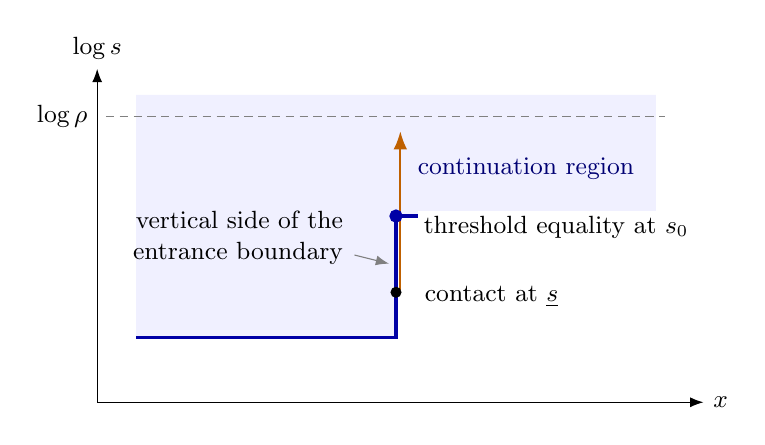
\begin{tikzpicture}[x=1.1cm,y=1.1cm,>=Latex,font=\small]
 \fill[blue!6] (-3,.75)--(0,.75)--(0,2.15)--(3,2.15)--(3,3.55)--(-3,3.55)--cycle;
 \draw[->] (-3.45,0)--(3.55,0) node[right] {$x$};
 \draw[->] (-3.45,0)--(-3.45,3.85) node[above] {$\log s$};
 \draw[blue!65!black,very thick] (-3,.75)--(0,.75)--(0,2.15)--(3,2.15);
 \draw[densely dashed,gray] (-3.35,3.3)--(3.1,3.3);
 \node[left] at (-3.45,3.3) {$\log\rho$};
 \node[blue!45!black] at (1.5,2.7) {continuation region};
 \node[anchor=east,align=right] at (-.5,1.9) {vertical side of the\\entrance boundary};
 \draw[->,gray] (-.48,1.7)--(-.08,1.6);
 \draw[orange!75!black,thick,->] (.05,1.3)--(.05,3.13);
 \fill (0,1.27) circle (2pt);
 \node[right] at (.22,1.22) {contact at $\underline s$};
 \draw[fill=white,blue!65!black,thick] (0,2.15) circle (2pt);
 \node[right,fill=white,inner sep=2pt] at (.25,2.02) {threshold equality at $s_0$};
\end{tikzpicture}
\caption{A schematic entrance boundary. In this illustration the contact
scale is denoted by $\underline s$ and a larger threshold scale by $s_0$.
A contact on a vertical side can have
derivative scale $\underline s<s_0$, where $s_0$ is a larger threshold scale.
The contact rule controls the initial derivative and the cumulative integral
along the outward vertical. It does not impose a pointwise sign at every later
scale. The two scales remain distinct in the final mass charge.}
\label{fig:contact}
\end{figure}


\subsection{Localization of the signed source}

All extensions in the next statement are made consistently: if $L'$ is
restricted to a working chart, $\tau$ is restricted to the same or a
larger chart, so that $|L'|\le C_0\tau$ survives extension by zero.
The constant density $d\,\dd y$ is placed on the entire torus.

\begin{lemma}[Uniform weight localization]\label{ct:localization}
Let $|L'|\le C_0\tau$, where $\tau$ is a finite positive measure on a
torus of diameter comparable to $R$, and let
$0\le w\le1$, $\Lip w\le R^{-1}$.  Put
\[
 \nu=\tau+d\,\dd y,\qquad f=wL'-\eta\nu,
 \qquad 0<\eta<1.
\]
Suppose, for some fixed $C_1$, that
$\tau(X)/(dR^m)\le e^{C_1T}$.  For all sufficiently large $T$, if
\begin{equation}\label{ct:localization-scale}
 0<\rho\le c\eta^2R/T^2,
\end{equation}
then, uniformly for every $x\in X$ and $0<s\le\rho$,
\begin{equation}\label{ct:localized-source}
 f_s(x)\le w(x)L'_s(x)-\frac\eta2\bigl(\tau_s(x)+d\bigr).
\end{equation}
Here $c>0$ depends only on $C_0,C_1$ and the fixed torus shape.
If $\sigma,h$ are furnished by \Cref{ct:contact} with contacts at
scales $s_0\le\rho$, then $w(x)>0$ at each contact, and
\begin{align}
 L'_{s_0}(x)&\ge h_{s_0}(x)+\tfrac\eta2\nu_{s_0}(x),
 \label{ct:localized-initial}\\
 \int_{s_0}^s v^2\bigl(L'-\tfrac\eta2\nu\bigr)_v(x)
 \,\dd\log v&\ge0\qquad(s_0\le s\le\rho).
 \label{ct:localized-cumulative}
\end{align}
In particular, contacts lie in the interior region containing
$\{w>0\}$.  These conclusions are uniform as the bottom scale tends to
zero.
\end{lemma}

\begin{proof}
The only commutator is
\[
 f_s(x)=w(x)L'_s(x)-\eta\nu_s(x)+E_s(x),\qquad
 |E_s(x)|\le C_0\int G_s(x-y)|w(y)-w(x)|\,\dd\tau(y).
\]
Split at torus distance $r_*=c_0\eta R$.  For sufficiently small fixed
$c_0$, the near contribution is at most $\eta\tau_s(x)/4$.
The far contribution is at most
\[
 C\tau(X)s^{-m}\exp(-c_2\eta^2R^2/s^2).
\]
Writing $x_*=s/R$, its ratio to $d$ is bounded by
$Ce^{C_1T}x_*^{-m}e^{-c_2\eta^2/x_*^2}$.
On $0<x_*\le c\eta^2/T^2$ this is $o(\eta)$ uniformly:
the negative exponent is at least a fixed multiple of $T^4/\eta^2$,
which dominates $C_1T$, $m|\log x_*|$, and $|\log\eta|$.
The same estimate applies to the nonnearest periodized copies.
This proves \eqref{ct:localized-source}.

At a contact $f_{s_0}\ge h_{s_0}\ge0$.  If $w(x)=0$,
\eqref{ct:localized-source} would give a strictly negative value.
Division by $w(x)>0$, followed by $w(x)\le1$, proves
\eqref{ct:localized-initial}.  Integrate
\eqref{ct:localized-source}, use the cumulative contact inequality and
the nonnegativity of the corresponding integral of $h$, and again
divide by the fixed number $w(x)$.  This proves
\eqref{ct:localized-cumulative}.
\end{proof}

The elementary proof just given requires no positive lower bound on
$s$.  In applications of first variation we also cut off the Gaussian
test field within the original chart.  If $s\le\rho\ll R$ and its
center lies in the fixed interior region, this introduces a factor
$\exp(-cR^2/s^2)$ times the bounded chart mass and fixed powers of
$s^{-1}$.  The same reasoning makes these errors smaller than any
prescribed part of the subtractive margin.  At a node of the recursion
below, $s\ge r_b$ and $\rho/R=T^{-4N}$, so this remains true even after
the factor $s^{-m}\le\exp(O(T))$ is included.  All subsequent Gaussian
identities use this convention.

\subsection{The estimate for separated configurations}

We use the signed estimate \Cref{sx:signed} only at smaller integers in
this subsection.  Separation refers to the scaled normal coordinates;
the integrands defining $\Lambda$ continue to use physical units.
In this subsection write $z=\zeta=z_{\rm phys}/l$, in the root chart;
these height coordinates remain fixed at all recursive nodes.

For two lists $\mathcal A=\{a_1,\ldots,a_Q\}$ and
$\mathcal B=\{b_1,\ldots,b_Q\}$, write
\[
 d_\infty(\mathcal A,\mathcal B)
 =\min_{\sigma\in\mathfrak S_Q}\max_{1\le j\le Q}|a_j-b_{\sigma(j)}|.
\]
Thus repetitions are distinct entries in a matching. Choose once
$0<r_{\rm maj}<1$ so that the fixed enlargements needed first to select
the integer by \Cref{lt:scalar} and then to apply \Cref{lt:config} on
the inner ball $B_{r_{\rm maj}}$ lie in $B_4$.
The corresponding inner ball of a work ball $B_r(y)$ is
$B_{r_{\rm maj}r}(y)$.

We use comparison chains whose work radii change by factors at most two
and whose center steps are at most one quarter of the smaller inner
radius. For adjacent inner balls $B,B'$, these choices give a fixed
$\vartheta_{\rm ov}>0$ such that
\begin{equation}\label{ct:majority-overlap}
 \vol_S(B\cap B')\ge
 \vartheta_{\rm ov}\bigl(\vol_S(B)+\vol_S(B')\bigr).
\end{equation}
Indeed their intersection contains a ball of a fixed fraction of the
smaller radius, and their radii are comparable. Fix
$0<\delta_{\rm maj}<\vartheta_{\rm ov}$, and let $C_{\rm maj}$ be a fixed
constant valid in \Cref{lt:config} for this exceptional proportion and
the finitely many fixed enlargements used below. Every auxiliary
configuration below uses this same exceptional proportion. The corresponding
smallness threshold in \Cref{lt:config} is therefore fixed before $T$;
the local bounds used to select these configurations tend to zero with $T$.

Suppose $s^{-m}\tau(B_{cs}(x))\le d_{\rm loc}$ on a ball and its required
fixed enlargement. A \emph{majority configuration} on $B_s(x)$ is a list
of $Q$ heights such that, outside a set of base volume at most
$\delta_{\rm maj}\vol_S(B_s(x))$, each fiber has exactly $Q$ projection
entries and these entries match the list within
$C_{\rm maj}s\sqrt{d_{\rm loc}}$. The projection entries repeat each
spatial point according to its integer multiplicity. If majority
configurations $\mathcal A,\mathcal B$ on adjacent balls of radii $s,t$
have local upper bounds $d_s,d_t$, then
\begin{equation}\label{ct:majority-matching}
 d_\infty(\mathcal A,\mathcal B)
 \le C_{\rm maj}\bigl(s\sqrt{d_s}+t\sqrt{d_t}\bigr).
\end{equation}
In fact, \eqref{ct:majority-overlap} leaves a fiber outside both
exceptional sets. Composing its two matchings proves the estimate,
including repetitions.

At the root the inner ball is $B_{r_{\rm maj}}$ and
$d_{\rm loc}=r_{\rm maj}^{-m}d$, so its matching error is a fixed
multiple of $\sqrt d$. The majority property itself imposes no condition
on exceptional fibers; their contribution remains in the global $\tau$
budget. A partition of a list's entries into groups is separated by
$\delta$ if different groups have mutual distance at least $\delta$.
Identical list entries therefore belong to the same group when $\delta>0$.

\begin{proposition}[Separated configurations]\label{ct:separated}
Fix $Q>1$ and assume \Cref{sx:signed} for every integer $1\le q<Q$.
For each fixed $P>0$ there are constants $C_Q,C_S$ and a function
$b=b_Q$ satisfying
\begin{equation}\label{ct:b-choice}
 b(T)\gg(\log T)^{200},\qquad b(T)=T^{o(1)},\qquad
 F_{Q-1}(b(T)/2)\ge(\log T)^3
\end{equation}
such that the following holds.  Under the hypotheses of
\Cref{sx:signed}, let $\mathcal A=\{a_1,\ldots,a_Q\}$ be any majority
configuration on $B_{r_{\rm maj}}$ with local upper bound
$d_{\rm loc}=r_{\rm maj}^{-m}d$, and suppose it has a partition into at least two
nonempty groups separated by
$10S(T)\sqrt d$, where
\[
 S(T)=e^{C_Sb(T)},\qquad c(T)=\frac{(\log T)^2}{T}.
\]
Let $D_{\rm far}$ be the projection of tilt restricted to
$\{\dist(z,\mathcal A)>S(T)\sqrt d\}$.  Then every nonnegative weight
$w\le1$, supported in $B_1$ with $\Lip w\le1$, satisfies
\begin{equation}\label{ct:separated-estimate}
 \int w\,\dd\bigl(L-C_Q\Lambda+c(T)D_{\rm far}\bigr)
 \le T^{-P}d.
\end{equation}
The statement holds on other fixed interior balls after rescaling.
Polynomial factors in the Lipschitz norm or the enlargement of a
Gaussian working ball can be allowed by increasing $P,C_S$ and the
fixed constants.
\end{proposition}

\begin{proof}
The proof is a finite recursion over working balls, with the root
configuration and its far-tilt region kept fixed. On a sufficiently
small ball, the support lies in disjoint neighborhoods of the root
groups. Cutting through the gaps gives stationary pieces with positive
counts below $Q$, so the lower-integer theorem makes the signed integral
small on that ball.

On a larger ball, if the signed integral exceeds a small margin, the
remaining positive source gives a contact measure.
The cumulative contact inequality and the Gaussian mass identity exclude
a contact whose derivative scale is close to a threshold hit or a side
equality: it would force too much signed mass at the outer scale.
Bottom contacts are excluded by the small-ball reduction. Each remaining
contact lies on a vertical side, far below its equality scale. Its signed
Gaussian integral is partitioned over smaller working balls, while a choice of thresholds
made before constructing the contact measure confines the associated
charging balls to a small part of the measure on the working ball. Thus a large
generation pays a small margin and at most half of the next-generation
bound. The choices below enforce these alternatives and keep the
configuration motion smaller than the original separation.

For example, after extending $F_{Q-1}$ monotonically over a fixed
initial interval, one can use
\[
 b(T)=1+(\log T)^{201}
       +4F_{Q-1}^{-1}((\log T)^3).
\]
The definition of the iterated exponentials gives
$F_{Q-1}^{-1}((\log T)^3)=T^{o(1)}$, and this choice has
\eqref{ct:b-choice}.  All changes of $b$ below are by fixed constants
or an additional fixed power of $\log T$.

Choose a fixed integer $N>P+10$, increasing it later if necessary, and
then choose a fixed $J_0$ sufficiently large in terms of $m,n,Q,N$.
In particular require
\begin{equation}\label{ct:J-choice}
 J_0>4N(m+2)+100,
\end{equation}
and enlarge $J_0$ to exceed all fixed polynomial density losses in the
cell constructions below.  Set
\begin{equation}\label{ct:recursion-parameters}
 \eta=T^{-N},\quad \varepsilon=\frac{(\log T)^{60}}{T},\quad
 r_b=\sqrt d\,e^{3b},\quad n_0=\lceil10N\log T\rceil,
 \quad E_j(t)=T^{J_0(j+1)}d\,t^{-2-\varepsilon}.
\end{equation}
The parameter $T$, the original configuration $\mathcal A$, and the
measure $D_{\rm far}$ remain fixed throughout the finite recursion.
They are never recomputed at a child node.

Two elementary parameter bounds will be used repeatedly.  With
$\ell_T=\log T$, direct substitution gives
\begin{equation}\label{ct:small-envelope}
 \log E_{2n_0+4}(r_b/T^4)
 =-6b+\tfrac12\ell_T^{60}-3\varepsilon b
       +O_{J_0,N}(\ell_T^2)
 <-2b.
\end{equation}
Also, for $i\le n_0$,
\begin{equation}\label{ct:motion-budget}
 v\sqrt{E_{2i+1}(v)}
 =\sqrt d\,T^{J_0(i+1)}v^{-\varepsilon/2}.
\end{equation}
For $v\ge cr_b/T^2$, the logarithm of the factor multiplying $\sqrt d$
is $O_{J_0,N}((\log T)^2)+O((\log T)^{60})$.  Consequently $O(T)$
such increments, even with any fixed polynomial loss in $T$, sum to
less than $e^b\sqrt d$.  This is why the much larger separation
$e^{C_Sb}\sqrt d$ survives every generation.

At generation $i$ a node consists of a ball $B_{4R}(x_*)$ with
\begin{equation}\label{ct:node-hypotheses}
 \tau(B_{4R}(x_*))\le C R^mE_{2i}(R),\qquad
 R\ge cr_b/T^2,
\end{equation}
and a majority configuration $\mathcal A_R$ on
$B_{r_{\rm maj}R}(x_*)$, with local upper bound
$C r_{\rm maj}^{-m}E_{2i}(R)$, satisfying
\[
 d_\infty(\mathcal A_R,\mathcal A)\le(i+1)e^b\sqrt d.
\]
The integer is $Q$ on the balls constructing the node; the small-density
and overlap checks below establish this before their configurations are
selected. We estimate all weights
$0\le w\le1$, $\Lip w\le R^{-1}$, supported in $B_R(x_*)$.
Write
\[
 L'=L-C_Q\Lambda+c(T)D_{\rm far},\qquad
 \mathcal N_R=\tau(B_{4R}(x_*))+dR^m.
\]
We prove, by downward induction on $i$, that
\begin{equation}\label{ct:node-conclusion}
 \int w\,\dd L'\le p_i\mathcal N_R,
 \qquad p_{n_0}=C_*,\qquad
 p_i=C\eta+\tfrac12p_{i+1}.
\end{equation}
Here $C_*,C$ are fixed, independent of $i$ and $T$.  The last-generation
bound follows at once from $|L'|\le C\tau$.  Initialization at $R=1$
follows from $\tau(B_4)\le d$ and the given configuration.

\paragraph{Small nodes and actual stationary pieces.}
Suppose first that $R\le T^{10N}r_b$, and put $E=E_{2i}(R)<1$,
as follows from \eqref{ct:small-envelope}.
Cover $B_{2R}(x_*)$ by a fixed finite number of balls of radius
$\sigma R$, including the concentric ball, where the fixed $\sigma>0$
is small enough that every
fixed enlargement needed for scalar selection and then for the support
estimate in \Cref{lt:config} lies in $B_{4R}(x_*)$, and the scalar
enlargement of the concentric ball lies in $B_{2R}(x_*)$.
Their normalized $\tau$ is at most $CE$.
The normalized smooth mass averages therefore differ from $Q$ by
$O(E)<1/4$, so \Cref{lt:scalar} selects $Q$ on these balls.
On each choose the joint configuration in \Cref{lt:config} with
exceptional proportion $\delta_{\rm maj}$, retaining its majority property
and using its all-support bound with a fixed
$0<\beta<\min\{1/2,1/m\}$. Its local upper bound is $CE=o(1)$.
Connect it to $\mathcal A_R$ by a fixed chain satisfying
\eqref{ct:majority-overlap}. The intermediate balls have the same
$CE=o(1)$ upper bound, and the same smooth mass test selects $Q$ there.
Equation \eqref{ct:majority-matching}
bounds this change by $CR\sqrt E$, while the support bound is $CRE^\beta$.
Consequently all support heights over $B_{2R}(x_*)$ satisfy
\begin{equation}\label{ct:bottom-sup}
 \begin{split}
 \dist(z,\mathcal A)
 &\le (i+1)e^b\sqrt d+CR\sqrt E+CRE^\beta\\
 &\le (i+1)e^b\sqrt d+C R E_{2i}(R)^\beta
 \le e^{C'b}\sqrt d
 \end{split}
\end{equation}
for a fixed $C'$. The second line uses $\beta<1/2$ and $E<1$.
To see the last bound without a
hidden scale restriction, write $R=\sqrt d\,e^{3b}T^\theta$, where
$-3\le\theta\le10N$, and substitute in $RE_{2i}(R)^\beta$;
its logarithm after division by $\sqrt d$ is bounded above by $C'b$
using \eqref{ct:small-envelope}.  Choose $C_S>C'+10$.
For a root group $\mathcal A_g$, put
\[
 \mathcal O_g=\{z:\dist(z,\mathcal A_g)<2S(T)\sqrt d\}.
\]
For large $T$, \eqref{ct:bottom-sup} puts all the support over $B_{2R}$
inside the smaller regions with radius $S(T)\sqrt d$. The regions
$\mathcal O_g$ are disjoint, since the root group gap is
$10S(T)\sqrt d$. Thus there is an open height gap around each group's
support, and no far energy in this interior region.

The use of disjoint height regions to obtain stationary restrictions
has a precedent in \cite[Section~3.1]{BDD2025}. For each group, restrict
the varifold over $B_{2R}(x_*)$ to $\{z\in\mathcal O_g\}$. Choose a
smooth height cutoff equal to one near the smaller region of radius
$S(T)\sqrt d$ around $\mathcal A_g$ and zero outside $\mathcal O_g$.
Its derivative vanishes near the entire support over $B_{2R}(x_*)$.
Multiplying any ambient test field with compact base support there by
this cutoff proves stationarity of the restriction. It keeps every
included spatial point with
its entire integer multiplicity, including on exceptional fibers.
On a majority fiber of one of the local configurations, its matching
to the fixed root list moves each entry by at most
$(i+1)e^b\sqrt d+CR\sqrt E=o(S(T)\sqrt d)$. An entry matched to
$\mathcal A_g$ therefore lies in $\mathcal O_g$. If two copies of one
spatial point were matched to different root groups, their two root
entries would be separated by at most twice this error, less than
$10S(T)\sqrt d$ for large $T$, contrary to the separation.
Each group's projection count on that fiber is thus
the number $q_g$ of entries in its root group, including repetitions.
Since there are at least two nonempty groups,
$1\le q_g<Q$ and $\sum_gq_g=Q$. To specify the individual energy budgets,
take a finite nonnegative partition of the weight on balls
$B_{r_\alpha}(y_\alpha)$, with $r_\alpha=cR$ for a sufficiently small
fixed $c$, and $B_{8r_\alpha}(y_\alpha)\subset B_{2R}(x_*)$.
These enlarged balls have bounded overlap. For each stationary
restriction, its normalized projected mass is bounded by the normalized total
mass, and its normalized $D+\Lambda$ is $O(E)=o(1)$. Apply
\Cref{lt:scalar} with its initial intermediate ball equal to the
concentric majority ball above. Its selected integer is $q_g$ by
intersection with the group majority set there. Connect this ball to
the intermediate balls for the scalar applications on
$B_{4r_\alpha}(y_\alpha)$ by a fixed finite chain of comparable
interior balls with the positive overlap in \eqref{ct:majority-overlap}.
The scalar count exceptions on each intermediate ball have relative
volume $O(E)$, smaller than the fixed overlap for
large $T$; on a remaining fiber the two selected integers coincide.
Thus $q_g$ is identified and propagated before the mass defect of the
restriction is estimated.

Write $\mu_g$ for the mass measure of the restriction and $D_g,\Lambda_g$
for its projected energy measures. Now set
$M_g=\pi_\#\mu_g-q_g\vol_S$ and $\tau_g=|M_g|+D_g+\Lambda_g$.
The scalar estimate with interior
room now gives
\[
 \tau_g(B_{4r_\alpha}(y_\alpha))
 \le C_s(D_g+\Lambda_g)(B_{8r_\alpha}(y_\alpha)).
\]
Define the parameter for the lower-integer application of \Cref{sx:signed} by
\begin{equation}\label{ct:group-budget}
 d_{g\alpha}=\max\left\{d,
 C_s r_\alpha^{-m}(D_g+\Lambda_g)
                  (B_{8r_\alpha}(y_\alpha))\right\},
 \qquad T_{g\alpha}=-\log d_{g\alpha}.
\end{equation}
Increasing the fixed $C_s$ if necessary supplies the required bound
for $\tau_g$ on each rescaled $B_4$.  Moreover
\begin{equation}\label{ct:group-budget-sum}
 \sum_{g,\alpha}d_{g\alpha}r_\alpha^m
 \le C\bigl((D+\Lambda)(B_{4R})+dR^m\bigr)
 \le C\mathcal N_R.
\end{equation}
Here the group energies add exactly on their separated region, and
the enlarged base balls have bounded overlap.  Individual mass defects
have been estimated by \Cref{lt:scalar}, rather than by splitting
$|M|$.  The parameters satisfy
\begin{equation}\label{ct:child-parameter}
 b/2\le T_{g\alpha}\le T.
\end{equation}
Indeed $d\le d_{g\alpha}\le d+C E_{2i}(R)$, and
\eqref{ct:small-envelope} absorbs the fixed constants.  Physical
radii only decrease, and physical heights are unchanged, so the
curvature hypothesis follows from the original one.  Apply
\Cref{sx:signed} at $q_g$ to the partition weights normalized by a
fixed constant.
Taking $C_Q$ at
least as large as the finitely many constants for $q<Q$, summing the
lower-integer conclusions with \eqref{ct:group-budget-sum} gives an
$o(\eta)\mathcal N_R$ bound.  Indeed
$F_q(T_{g\alpha})\ge F_{Q-1}(b/2)\ge(\log T)^3$ for large $T$.
This argument also applies to the small cells used at a bottom contact.

\paragraph{Stopping tests at a large node.}
Now assume $R>T^{10N}r_b$.  Use a torus of period $C R$, identifying
the node and a fixed surrounding chart with its central portion.  Put
\[
 \nu=\tau|_{B_{4R}(x_*)}+d\,\dd y,
 \qquad \rho=T^{-4N}R.
\]
Its total mass is comparable to $\mathcal N_R$.  If
$f=wL'-\eta\nu$ has nonpositive integral there is nothing to prove.
Otherwise apply \Cref{ct:contact} with bottom $r_b$ and dyadic test
scales $t\in[r_b,\rho]$, using
\begin{equation}\label{ct:stopping-q}
 q_t(x)=\frac{(\tau|_{B_{4R}(x_*)})_t(x)}{E_{2i+1}(t)},
 \qquad q_t(x)\le\lambda_t,\quad 1\le\lambda_t\le2.
\end{equation}
The thresholds will be chosen later.  There are $O(T)$ test scales.
The torus masses satisfy the growth condition in
\Cref{ct:localization}, because
$\mathcal N_R/(dR^m)\le\exp(O(T))$ by
\eqref{ct:node-hypotheses}.  Also
$\rho/R=T^{-4N}\ll\eta^2/T^2$.

For every contact $(x,s_0)$, localization places $x$ in the interior
support region.  Gaussian comparison between successive dyadic scales,
and the non-strict tests at larger scales, give
\begin{equation}\label{ct:contact-envelope}
 \tau_v(x)\le C E_{2i+1}(v)\qquad(s_0\le v\le\rho).
\end{equation}
Here and below the measure in this display is the node restriction.
At the current mesh scale its value is bounded by the next larger
scale.  At the top use the node's total mass.  In fact, for
$v\ge\rho/16$,
\[
 q_v(x)\le C T^{-J_0}(R/v)^{m-2-\varepsilon}
 \le C T^{-J_0+4N\max(m-2,0)}.
\]
Thus all top tests hold strictly, and every scale with $q_v\ge1$
lies below $\rho/16$, leaving a fixed outward interval below $\rho$.

If $s_0>r_b$, the boundary description
\eqref{ct:mesh-domain} supplies a mesh scale $v_1\ge s_0$ with
$q_{v_1}(x)\ge1$.  Either it is a current hit, or it is a larger scale
with $q_{v_1}(x)=\lambda_{v_1}$.  In the latter case every still larger
test satisfies its continuation inequality.  This follows directly
from the finite intersection: away from the bottom, if there were no
current obstruction and every relevant larger test were strict, a
space--scale neighborhood would belong to $\mathcal D$.

\paragraph{Exclusion of a nearby hit or side equality.}
We show that no such $v_1$ can satisfy
$v_1/s_0\le(\log T)^{20}$.  All the following estimates are on this
one outward vertical.  Put
\[
 I_1=v_1^2E_{2i+1}(v_1),\qquad A(v)=v^2M_v(x),\qquad
 Z(s)=\int_{s_0}^s v^2(L'-\tfrac\eta4\nu)_v(x)\,\dd\log v.
\]
By \Cref{ct:localization}, $Z\ge0$ and $A(s_0)\ge0$; the latter
uses $c(T)<1$ and $L'=2M-D-C_Q\Lambda+c(T)D_{\rm far}$.
The envelope gives
\begin{equation}\label{ct:nearhit-cost}
 \int_{s_0}^{\rho}v^2D_v\,\dd\log v
 \le \frac{C I_1}{\varepsilon}
          (v_1/s_0)^\varepsilon
 \le \frac{C I_1}{\varepsilon},
 \qquad \frac{c(T)}\varepsilon=(\log T)^{-58}.
\end{equation}
In particular the adverse $c(T)D_{\rm far}$ term is small enough for
the logarithmic losses below.

At $v_1$, and on its fixed outward dilations, the scalar estimate is
available in weighted form:
\begin{equation}\label{ct:nearhit-scalar}
 |M|_{v_1}\le C(D+\Lambda)_{v_1}+o(E_{2i+1}(v_1)).
\end{equation}
Here are the raw density and integer checks, also needed for the
children below.  For $s\in[s_0,\rho]$ and
$U=1+|y-x|/s\le C\sqrt T$, put $r=cs/U$ with a small fixed $c$.
All required fixed enlargements $B_{Lr}(y)$ lie in $B_{2R}(x_*)$:
$x\in B_R(x_*)$ and $C\sqrt T\,\rho=o(R)$.  Choose
$a=C_1Us$ so that $G_a(x-z)\ge c_1a^{-m}$ on these enlarged balls.
If $a\le\rho$, positivity and the envelope give
\[
 r^{-m}\tau(B_{Lr}(y))
 \le C(a/r)^m E_{2i+1}(a)
 \le C U^{2m-2-\varepsilon}E_{2i+1}(s).
\]
If $a>\rho$, use the node total instead.  Dividing by
$E_{2i+1}(s)$ gives the bound
\[
 C T^{-J_0}U^m(R/s)^{m-2-\varepsilon}
 \le C T^{-J_0+4N\max(m-2,0)}
             U^{m+\max(m-2,0)}\le C.
\]
In the middle inequality a negative exponent of $R/s$ is discarded;
for a positive exponent use $R/s\le C U T^{4N}$.
Consequently, in both cases,
\begin{equation}\label{ct:cell-density}
 r^{-m}\tau(B_{Lr}(y))
 \le C T^{\max(m-1,0)}E_{2i+1}(s)=o(1).
\end{equation}
Since $\tau$ includes $|M|=|\pi_\#\mu-Q\vol_S|$, choose a fixed
nonnegative smooth mass test on this enlarged ball, normalized to
reference integral one and with bounded scaled derivatives.  Its
average differs from $Q$ by at most the right side times a fixed
constant, hence by less than $1/4$.  This identifies $Q$ directly
in \Cref{lt:scalar}, and also
provides its mass and energy hypotheses.  Apply \Cref{lt:scalar} at $s=v_1$
on a cover by these cells and sum with the comparable Gaussian
weights, as in \Cref{lt:weightedballs}.  The cutoff at
$C\sqrt T\,v_1$ has arbitrarily small exponential tail for a large
fixed $C$, using the node total and $v_1\ge r_b$.

The identity in \Cref{lt:gaussian}, integrated using the nonnegative
bank $Z$, gives
\begin{equation}\label{ct:nearhit-bank}
 A(s)\ge A(s_0)+\int_{s_0}^s v^2R_v\,\dd\log v+Z(s)
             -C(\log T)^{-58}I_1,
 \qquad s_0\le s\le\rho.
\end{equation}
The geometric errors are absorbed by part of the remaining margin
$\eta\nu/4$: on $|u|\le T$ they carry the factor
$Ce^{-\kappa T}(1+T^2)=o(\eta)$, and the tails are negligible under
\eqref{ct:contact-envelope} and the node total.  The nonnegative
$C_Q\Lambda$ term has been discarded.

There is a fixed $c_1>0$ such that $A(v_1)\ge c_1I_1$.
This includes a current hit with $q_{v_1}>\lambda_{v_1}$: although
its current test is omitted, the next larger mesh scale $t_+\le2v_1$
obeys $\tau_{t_+}\le2E_{2i+1}(t_+)$, and
$G_{v_1}\le(t_+/v_1)^mG_{t_+}$ bounds its current average.
Only $q_{v_1}\ge1$ is needed for the lower bound.

For an explicit cumulative-sign argument, fix $C_Q\ge1$ first and
let $C_s$ be the constant in \eqref{ct:nearhit-scalar}.  Write
$E_1=E_{2i+1}(v_1)$ and take $T$ large enough that its tail is at
most $E_1/2$ and $c(T)\le1/2$.  Then
\[
 (D+\Lambda)_{v_1}\ge\alpha E_1,
 \qquad \alpha=\frac{1}{2(C_s+1)}.
\]
If $A(v_1)\le c_1I_1$ with $c_1\le\alpha/8$, then
$L'_{v_1}\le2c_1E_1-(D+\Lambda)_{v_1}/2\le-\beta E_1$,
where $\beta=\alpha/4$.  For
$v\in[v_1,2^{1/4}v_1]$, differentiating the fixed source $L'$
and dominating $|\dot G_v|$ by $CG_{2v}$ gives
$|\dot L'_v|\le K_1E_1$.  The constant $K_1$ is fixed after $C_Q$;
the envelope at $2v$ follows from strictly larger mesh tests, and
$v_1<\rho/16$ leaves room.  In particular this estimate does not
use the omitted current test or differentiate the fixed far cutoff.
Choose
\[
 \theta=\min\{\tfrac14\log2,\beta/(2K_1)\},\qquad
 \gamma=\beta\theta/2,\qquad
 0<c_1\le\min\{\alpha/8,\gamma/4\}.
\]
On $[v_1,e^\theta v_1]$ one has $L'_v\le-\beta E_1/2$,
hence $\dot Z\le-\beta I_1/2$.  Nonnegativity of $Z$ at the
right endpoint gives $Z(v_1)\ge\gamma I_1$.
Finally take $T$ large enough that the error in
\eqref{ct:nearhit-bank} is at most $\gamma I_1/2$.
That inequality at $v_1$ yields $A(v_1)\ge\gamma I_1/2>c_1I_1$,
a contradiction.  All constants were fixed before this last largeness
threshold; only the cumulative sign of $Z$ was used at later scales.

The upper differential inequality
$\dot A\le2A+v^2R_v+$ absorbed errors, again from
\Cref{lt:gaussian}, and $v_1/s_0\le(\log T)^{20}$ now yield
\begin{equation}\label{ct:nearhit-surplus}
 A(s_0)+\int_{s_0}^{v_1}v^2R_v\,\dd\log v
 \ge c(\log T)^{-40}I_1.
\end{equation}
One may retain the geometric error explicitly in the integrating
factor formula: divided by $I_1$ it is
$O(e^{-\kappa T}T^C/\varepsilon)$, hence smaller than every fixed
inverse power of $\log T$.  Inserting
\eqref{ct:nearhit-surplus} in \eqref{ct:nearhit-bank} at $\rho$
gives $A(\rho)\ge c(\log T)^{-40}I_1$.  On the other hand the
node mass gives
\[
 A(\rho)\le C\rho^2(R/\rho)^m E_{2i}(R)
   = C T^{J_0(2i+1)+4N(m-2)}dR^{-\varepsilon},
 \qquad I_1=T^{J_0(2i+2)}dv_1^{-\varepsilon}.
\]
The ratio of the upper bound to $I_1$ is at most
$CT^{-J_0+4N(m-2)}$, contradicting \eqref{ct:J-choice}.
This excludes current hits and all side equalities within the stated
logarithmic factor.

\paragraph{Gaussian children and the bottom.}
For any remaining contact, configurations on the Gaussian cells at
$s_0$ match the node configuration with movement at most $e^b\sqrt d$.
Here is the comparison chain for a cell with work radius comparable to
$s_0/U$, where $U=1+|y-x|/s_0\le C\sqrt T$. First shrink concentrically
at $x_*$ to a small fixed multiple of $R$, move the center to $x$ at
that radius, and then shrink concentrically to a work radius comparable
to $Us_0$. Move the center to $y$ at that radius and finally shrink to
the cell radius. At each stage change radii by factors at most two and
make center steps at most one quarter of the smaller inner majority
radius. All these inner balls satisfy \eqref{ct:majority-overlap}, so
\eqref{ct:majority-matching} bounds the changes by the sum of their
local matching errors. The initial fixed chain stays inside
$B_{4R}(x_*)$; the off-center chain at scale $s_0$ lies in
$B_{CUs_0}(x)\subset B_{2R}(x_*)$. The envelope bounds these increments by
\eqref{ct:motion-budget}, with fixed polynomial losses.  More
explicitly, above $\rho$ the node total gives, for
$\rho\le t\le cR$,
\[
 t\sqrt{t^{-m}\tau(B_{ct}(x))}
 \le C R\sqrt{E_{2i}(R)}\,
              T^{2N\max(m-2,0)}.
\]
Off-center balls nested from scale $Us_0$ down to $s_0/U$ have the
same increment bound as $s_0\sqrt{E_{2i+1}(s_0)}$, with another
fixed power of $U\le C\sqrt T$, by the raw estimates proving
\eqref{ct:cell-density}. All normalized bounds used for intermediate
configurations are at most a fixed power of $T$ times $E_{2i}(R)$ or
$E_{2i+1}(t)$ for $t\ge cr_b/T^2$. Hence they tend to zero by
\eqref{ct:small-envelope}. Their $|M|$ terms give the same smooth mass
test selecting $Q$, and \Cref{lt:config} is applied with the fixed
$\delta_{\rm maj}$ before each matching. The logarithms of all these factors are
$O_{J_0,N,m}((\log T)^2)+O((\log T)^{60})$ after division by
$\sqrt d$.  Since there are $O(T)$ steps,
\eqref{ct:motion-budget} proves the claimed $e^b\sqrt d$ allowance.

Here is the precise normalization of the cells.  A smooth partition of
unity on $|u|\le C\sqrt T$, where $u=(y-x)/s_0$, can be chosen with
bounded overlap on balls $B_{r_j}(y_j)$, with
\begin{equation}\label{ct:gaussian-cells}
 r_j\asymp\frac{s_0}{1+|y_j-x|/s_0},\qquad
 |\nabla\chi_j|\le C/r_j.
\end{equation}
Use a sufficiently small fixed constant in $\asymp$ to leave room for
$B_{4r_j}(y_j)$.  This follows, for example, by a maximal disjoint
selection for the Lipschitz radius function in
\eqref{ct:gaussian-cells}, followed by normalized smooth bumps.
On the enlarged ball, $G_{s_0}(x-y)$ differs from
$G_{s_0}(x-y_j)$ by a fixed factor, and its logarithmic gradient is
$O(r_j^{-1})$.  Thus
\[
 w_j(y)=\frac{\chi_j(y)G_{s_0}(x-y)}{C G_{s_0}(x-y_j)}
\]
is an admissible child weight after a fixed normalization.  In
particular, this normalization has no power of $T$.

The child's unweighted density was estimated in
\eqref{ct:cell-density}.  The identity
\[
 E_{2i+2}(r_j)=T^{J_0}E_{2i+1}(s_0)(s_0/r_j)^{2+\varepsilon}
\]
then gives
\[
 r_j^{-m}\tau(B_{4r_j}(y_j))
 \le C T^{\max(m-1,0)}E_{2i+1}(s_0)
 \le C E_{2i+2}(r_j),
\]
by the choice of $J_0$, with $C$ independent of $i,T$.
Also $r_j\ge cr_b/\sqrt T\ge cr_b/T^2$.
The smooth mass test following \eqref{ct:cell-density} identifies $Q$
on each child. After scaling its work ball to one, choose from
\Cref{lt:config} a majority configuration on $B_{r_{\rm maj}}$
with local upper bound $C r_{\rm maj}^{-m}E_{2i+2}(r_j)$.
Using the same normal frame, multiply its heights by $r_j$ to return
to the root coordinates.
The matching argument above gives its allowance relative to
$\mathcal A$, so these are admissible next-generation
nodes.  Although the raw density estimate loses a polynomial factor,
summation of the resulting estimates does not: bounded overlap and
Gaussian comparability give
\begin{equation}\label{ct:cell-sum}
 \sum_jG_{s_0}(x-y_j)
       \bigl[\tau(B_{4r_j}(y_j))+dr_j^m\bigr]
 \le C\bigl(\tau_{s_0}(x)+d\bigr).
\end{equation}
The fixed $d$ floors therefore sum to the correct constant-density
Gaussian average.

At a bottom contact $s_0=r_b$, these cells are small nodes.  The
stationary-piece argument above, including
\eqref{ct:child-parameter}, bounds $L'_{s_0}$ by
$o(\eta)\nu_{s_0}$.  The Gaussian tail outside $C\sqrt T$ is
$o(\eta)d$ for a sufficiently large fixed $C$: combine its
$e^{-C^2T/4}$ factor with total node mass and
$s_0^{-m}\le\exp(O(T))$.  This contradicts
\eqref{ct:localized-initial}; there are no bottom contacts.
At any other remaining contact the next-generation bound and
\eqref{ct:cell-sum} give
\begin{equation}\label{ct:child-contact-bound}
 h_{s_0}(x)\le C_0p_{i+1}\nu_{s_0}(x).
\end{equation}
All omitted tails are absorbed by the subtractive margin in
\eqref{ct:localized-initial}.  In particular, every remaining contact
is a vertical-side contact with some equality scale
\begin{equation}\label{ct:remote-side}
 v_1/s_0>(\log T)^{20}.
\end{equation}

\paragraph{First charging step: replace a Gaussian by a nearby ball.}
Put $J=\log T$ and $p=p_{i+1}$.  Call a contact $(x,s)$ good if some
closed ball of radius $0<r\le Js$ satisfies
\begin{equation}\label{ct:good-ball}
 h(\overline B_r(x))\le A_0p\nu(\overline B_r(x)),
\end{equation}
where $A_0\ge2C_0$ is a fixed constant.  Otherwise call it bad.
We first show that all bad centers together carry only
$o(\eta)\mathcal N_R$ mass of $h$.

For the Euclidean Gaussian, radial layer cake gives
\[
 \nu_s(x)=c_ms^{-m}\int_0^\infty
                  t e^{-t^2/2}\nu(B_{ts}(x))\,\dd t.
\]
At a bad contact the failure of \eqref{ct:good-ball} for every
$r\le Js$ bounds the part with $t\le J$ by $h_s/(A_0p)$.
Define the remaining layer-cake tail by
\[
 \mathcal T_{J,s}\nu(x)=c_ms^{-m}\int_J^\infty
                   t e^{-t^2/2}\nu(B_{ts}(x))\,\dd t.
\]
This is a tail in the layer-cake radius: it includes the residual
weight $c_ms^{-m}e^{-J^2/2}\nu(B_{Js}(x))$ as well as mass farther
away.  Combining
$\nu_s\le h_s/(A_0p)+\mathcal T_{J,s}\nu$ with
\eqref{ct:child-contact-bound} gives
\begin{equation}\label{ct:bad-tail}
 h(B_{5s}(x))\le C_m s^m h_s(x)
              \le C_mp s^m\mathcal T_{J,s}\nu(x).
\end{equation}

Let $E_{\rm bad}$ consist of spatial contact centers that admit no
good representative; for each of them assign one contact scale.
The elementary $5r$ covering lemma selects disjoint assigned balls
whose fivefold enlargements cover these centers.  Their scales lie in
$[r_b,\rho]$, hence in $O(T)$ dyadic bins.  In a bin $[a,2a)$,
disjointness implies, for every $y$ and $t\ge1$,
\[
 \sum_j\mathbf1_{B_{ts_j}(x_j)}(y)\le C_m(1+t)^m:
\]
the disjoint balls of radius at least $a$ have centers in a ball of
radius $Cta$.  Sum \eqref{ct:bad-tail}, use Tonelli, and then sum the
bins to obtain
\begin{equation}\label{ct:bad-total}
 h^*(E_{\rm bad})
 \le C_mpT(1+J)^{m+1}e^{-J^2/2}\nu(X)
 =o(\eta)\mathcal N_R.
\end{equation}
Here $h^*$ denotes outer measure, so no measurable choice of a contact
above each center is needed.  The same proof on the torus uses periodic
lifts of $h,\nu$: the small selected balls have disjoint lifts, the
packing estimate is unchanged, and the periodic Gaussian is exactly
the sum over those lifts.  Alternatively the nonnearest copies can be
absorbed in the exponentially smaller chart tail.

\paragraph{Second charging step: localize the union of good balls.}
Every good ball lies in a set determined only by the node's tests and
thresholds.  To see this, let $(x,s)$ be its contact and choose the
equality scale $v_1$ in \eqref{ct:remote-side}.  For every mesh scale
$v\ge v_1$ and every $|y-x|\le Js$, Gaussian differentiation gives
\begin{equation}\label{ct:q-gradient}
 |\nabla q_v(y)|\le C/v.
\end{equation}
Indeed $|\nabla G_v(y-z)|$ is bounded by
$Cv^{-1}G_{2v}(x-z)$ when $|y-x|\le v/10$; the envelope at $2v$
proves the assertion when $2v\le\rho$.  For $2v>\rho$ the node total
and the top slack following \eqref{ct:stopping-q} give the same bound.
Since $Js/v_1<J^{-19}$, for sufficiently large $T$ every point of
the good ball satisfies
\begin{equation}\label{ct:charged-tests}
 q_v(y)\le\lambda_v+\delta\quad(v>v_1),\qquad
 |q_{v_1}(y)-\lambda_{v_1}|\le\delta,
 \qquad\delta=J^{-15}.
\end{equation}

Order the mesh scales $v_1',\ldots,v_K'$ from largest to smallest,
and define the Borel set
\begin{equation}\label{ct:threshold-event}
 \mathcal E_\lambda=
 \bigcup_{k=1}^K\left[
  \{|q_{v_k'}-\lambda_{v_k'}|\le\delta\}
  \cap\bigcap_{j<k}\{q_{v_j'}\le\lambda_{v_j'}+\delta\}
                    \right].
\end{equation}
Equation \eqref{ct:charged-tests} says that every original good ball,
not just its center, lies in $\mathcal E_\lambda$.

We use the following form of the Besicovitch covering theorem
\cite[Chapter~1, Lemma~4.5]{Simon2018}.
For a bounded set with one assigned positive-radius ball at each
point and bounded assigned radii, there is a countable subfamily
covering the set by the original balls, with multiplicity bounded by
a dimensional constant $N_m$.  Arbitrarily small assigned radii are
allowed.  One proof groups the radii into dyadic bins and, in decreasing
bins, greedily selects uncovered centers.  The selected centers in
each bin are separated by that bin's minimum radius, so only finitely
many are needed in a bounded region.  For the overlap bound at a point,
divide directions into finitely many cones of angular diameter less
than $\pi/3$.  In a cone take the first selected center $x_i$ among
balls containing the point $y$.  For a later such center $x_j$, the
cosine law gives
$|x_i-x_j|<\max(|x_i-y|,|x_j-y|)\le\max(r_i,r_j)$.
Since $x_j$ was not covered by the earlier ball, $|x_i-x_j|>r_i$;
hence $r_j>r_i$.  The decreasing order of the dyadic bins forces
these two radii into the same bin.  Packing in that bin bounds the
number.  A selected center equal to $y$ contributes at most one
additional ball.  This proves the dimensional multiplicity bound.

Choose one good contact and one good ball above each center that has
such a representative, and apply this covering fact.  Since the
original balls lie in $\mathcal E_\lambda$, \eqref{ct:good-ball}
gives
\begin{equation}\label{ct:good-total}
 h^*(E_{\rm good})
 \le A_0p\sum_j\nu(B_j)
 \le A_0N_mp\nu(\mathcal E_\lambda).
\end{equation}
This is the reason for using original balls in this second covering;
the inequality \eqref{ct:good-ball} need not hold on an enlargement.

\paragraph{Choosing the thresholds.}
The measure $\nu$ and the functions $q_v$ are already fixed by the
node.  Choose independent thresholds at the mesh scales with
distribution function
\begin{equation}\label{ct:threshold-law}
 F(t)=
 \begin{cases}
 0,&t\le1,\\
 \exp\bigl(1-1/(t-1)\bigr),&1<t<2,\\
 1,&t\ge2.
 \end{cases}
\end{equation}
For every fixed $K_0>0$, uniformly in real $z$,
\begin{equation}\label{ct:threshold-probability}
 \mathbb P\{|\lambda-z|\le\delta\}
 \le T^{-K_0}+C_{K_0}(\log T)^{-13}F(z-\delta).
\end{equation}
If $F(z+\delta)\le T^{-K_0}$ this is immediate.  Otherwise, put
$a_*=(1+K_0\log T)^{-1}$.  One has $z+\delta-1\ge a_*$,
also when $z+\delta\ge2$, and consequently
$z-\delta-1\ge a_*-2\delta\ge a_*/2$ for large $T$.
Thus this case does not meet the lower endpoint $1$.  On the part
of $[z-\delta,z+\delta]$ below $2$ one has
$(\log F)'=(t-1)^{-2}\le4/a_*^2\le C_{K_0}(\log T)^2$;
above $2$, $\log F=0$.  Integration proves
$F(z+\delta)-F(z-\delta)
 \le C_{K_0}(\log T)^{-13}F(z-\delta)$.
Truncation at $2$ only decreases this difference.  This proves
\eqref{ct:threshold-probability}, including intervals meeting either
endpoint.

Fix $y$, and write $z_k=q_{v_k'}(y)$ and $r_k=F(z_k-\delta)$.
At the $k$th event in \eqref{ct:threshold-event}, all preceding
thresholds have survived, namely $\lambda_{v_j'}\ge z_j-\delta$.
Independence, \eqref{ct:threshold-probability}, and a union bound give
\begin{align*}
 \mathbb P\{y\in\mathcal E_\lambda\}
 &\le KT^{-K_0}
  +C_{K_0}(\log T)^{-13}
       \sum_{k=1}^K r_k\prod_{j<k}(1-r_j)\\
 &\le KT^{-K_0}+C_{K_0}(\log T)^{-13}=o(1).
\end{align*}
The sum telescopes to $1-\prod_k(1-r_k)\le1$; no disjointness of
the candidate events has been assumed.  Since $K=O(T)$, any fixed
$K_0>2$ suffices.  Integrating against the fixed measure $\nu$ and
using Tonelli supplies thresholds with
\[
 \nu(\mathcal E_\lambda)\le o(1)\nu(X).
\]
Choose such thresholds first, and only then construct the contact
measure.  This order makes independence explicit: the contact measure
may depend on the chosen thresholds, but neither $\nu$ nor $q_v$ does.
For large $T$, the last bound pays for $A_0,N_m$ and the fixed factor
between $\nu(X)$ and $\mathcal N_R$.  Equations
\eqref{ct:bad-total} and \eqref{ct:good-total} imply
\[
 h(X)\le\tfrac12p_{i+1}\mathcal N_R+o(\eta)\mathcal N_R.
\]
Because $h(X)=\int w\,\dd L'-\eta\nu(X)$, this is
\eqref{ct:node-conclusion} after increasing the fixed $C$.

Finally solve the recurrence:
\[
 p_0\le2C\eta+2^{-n_0}C_*,\qquad
 2^{-n_0}\le T^{-10N\log2}.
\]
At the initial node $\mathcal N_1\le2d$.  Increasing the fixed $N$
relative to the requested $P$ gives \eqref{ct:separated-estimate}.
There have been at most $n_0$ configuration changes, costing
$(n_0+1)e^b\sqrt d\ll S(T)\sqrt d$ in total.  Thus the fixed root
separation and far cutoff used at every step are valid.  A polynomial
weight or dilation loss is handled by starting with a correspondingly
larger $P$ and using the same Gaussian cell normalization.  This proves
the final assertion as well.
\end{proof}

\section{The outward envelope and the low-frequency barrier}
\label{sec:excess}

We continue the induction for \Cref{sx:signed} at the integer \(Q\).
Thus \Cref{ct:separated} is available when \(Q>1\), using only the
assertion at smaller integers. We shall construct a positive envelope
\(I(s)\) of future signed masses \(A(s)=s^2M_s\) and follow its
logarithmic level \(a(s)=\log(s^2/I(s))\). The output in
\Cref{ex:bands} is a traversal from \(a=B\) to \(a=2B\) in one of
\(Q\) fixed bands, with no merger of its height centers and with
\(k\ge B^{-\eps_0}\) for the coefficient \(k\) of the height moment,
where \(\eps_0>0\) is fixed and small. This holds for every contact
selected below whose outward vertical contains a threshold equality; \Cref{sec:packing}
will turn the traversal into many scales with normal flux.

All heights in this section are in the scaled coordinates of
\Cref{sx:signed}; the quantities defining
\(\Lambda\) retain their physical units. Gaussian averages are centered
at the contact under consideration. The dot denotes differentiation
with respect to \(t=\log s\).

Fix, in this order, a sufficiently large Gaussian exponent \(K>2m+100\),
a sufficiently large inverse-polynomial exponent \(P_0\), and the
constants in the separated estimate. They may depend on \(m,n,Q\) and
the fixed coordinate bounds. Increasing these fixed constants only
increases the lower threshold for \(T\). Put
\begin{equation}
 F=F_Q(T),\qquad \eta=e^{-2F},\qquad
 a_0=F^2,\qquad d_*=e^{-a_0},\qquad \rho=\eta^4T^{-2}.
 \label{ex:parameters}
\end{equation}
The elementary rate comparisons proved in \Cref{ex:bands} include
\(F=T^{o(1)}\), \(a_0=o(T)\), and \(|\log\rho|=o(T)\).

\subsection{Selection and the bottom boundary}

Extend the localized measures to the fixed torus of
\Cref{ct:localization}, and write \(\nu=\tau+d\,\dd y\), with
\(\tau\) restricted to a fixed interior enlargement of the working
set. For a weight \(w\) in \Cref{sx:signed}, use the source
\begin{equation}
 f=w(L-C_Q\Lambda)-\eta\nu.
 \label{ex:source}
\end{equation}
To prove the required upper bound it is enough to exclude
\(\int f\ge\eta d\): the total mass of \(\nu\) is at most \(Cd\),
and \((C+1)\eta\le e^{-F}\) for large \(T\).

Start at \(\rho\), continue downwards while \(\tau_s(x)\le d_*\),
and stop at a threshold equality or at a positive bottom \(\sigma\).
Use the continuous entrance boundary, including its vertical sides,
from \Cref{ct:contact}. At the top the continuation inequality is
strict, since \(\tau_\rho\le Cd\rho^{-m}=o(d_*)\).
Let \(K_\sigma\) denote this compact entrance boundary. Write
\(\widehat h_\sigma\) for its contact measure,
\(h_\sigma=(\pi_X)_\#\widehat h_\sigma\) for the spatial projection,
and \(\mathcal S_\sigma=\spt\widehat h_\sigma\). Both measures have
mass \(\int f\). In this section a contact means a point of
\(\mathcal S_\sigma\), where \Cref{ct:contact} supplies the pointwise
and cumulative contact inequalities. At every contact
\((x,\underline s)\),
\begin{equation}
 (h_\sigma)_{\underline s}(x)\le f_{\underline s}(x)
 \le Cd_*,\qquad
 \tau_v(x)\le d_*\quad(\underline s\le v\le\rho).
 \label{ex:threshold-control}
\end{equation}
Here and below source localization first places the contact in the
fixed interior region and gives \(w(x)>0\). The constants in
\eqref{ex:threshold-control} are independent of \(\sigma\).

Define the threshold event
\[
 \mathcal G_\sigma=
 \{(x,u)\in K_\sigma:\ \tau_v(x)=d_*
                 \text{ for some }v\in[u,\rho]\}.
\]
The corresponding set of \(((x,u),v)\) is closed in
\(K_\sigma\times[\sigma,\rho]\), by continuity of the Gaussian
averages. Its projection \(\mathcal G_\sigma\) is therefore compact
and Borel. The strict top inequality excludes \(v=\rho\). If a
boundary point above the bottom had no equality, the continuation
inequalities would be uniformly strict on its compact outward
interval; continuity would then make it an interior point. Hence
\(K_\sigma\setminus\mathcal G_\sigma\) consists precisely of bottom
points with no threshold equality.

\begin{lemma}[Vanishing contribution from the bottom]
\label{ex:bottom}
The mass \(\widehat h_\sigma(K_\sigma\setminus\mathcal G_\sigma)\)
is at most
\[
 o_{\sigma\downarrow0}(1)+Cd_*d.
\]
Every contact in \(\mathcal G_\sigma\) has a scale
\(s_0\in[\underline s,\rho)\) with
\(\tau_{s_0}(x)=d_*\). The inequalities
\eqref{ex:threshold-control} hold also when
\(\underline s<s_0\).
\end{lemma}

\begin{proof}
Only the first assertion needs proof. Put
\[
 \beta_\sigma=(\pi_X)_\#
       \bigl(\widehat h_\sigma\!\restriction_{K_\sigma\setminus\mathcal G_\sigma}\bigr)
       \le h_\sigma,
\]
and let \(\mathcal C_\sigma\) be the centers of contacts in
\(K_\sigma\setminus\mathcal G_\sigma\). Assign these contacts to grid
cubes of side \(\sigma\). If such a cube \(J\) contains a contact
\(x_J\), the Gaussian lower bound on \(J\), together with the contact
inequality, gives
\[
 h_\sigma(J)\le C\sigma^m(f_\sigma(x_J))_+
 \le Cd_*\sigma^m.
\]
Since \(\beta_\sigma\le h_\sigma\), this also bounds
\(\beta_\sigma(J)\). On an occupied half-open grid cube define
\[
 g_\sigma|_J=C\sup_{x\in\mathcal C_\sigma\cap J}
                   (f_\sigma(x))_+,
 \qquad
 \overline\beta_\sigma
   =\sum_J\frac{\beta_\sigma(J)}{|J|}\mathbf1_J\,\dd y,
\]
and put \(g_\sigma=0\) on unoccupied cubes. Then
\(\overline\beta_\sigma\le g_\sigma\,\dd y\) and
\(0\le g_\sigma\le Cd_*\). For every continuous test \(\varphi\),
\[
 \left|\int\varphi\,\dd\beta_\sigma
            -\int\varphi\,\dd\overline\beta_\sigma\right|
 \le\omega_\varphi(C\sigma)\beta_\sigma(\text{chart})\longrightarrow0,
\]
where \(\omega_\varphi\) is its modulus of continuity.

For a finite measure \(\lambda\), at almost every Lebesgue point of
its absolutely continuous density one has
\[
 \sup_{|x-y|\le C\sigma}
 \big|(G_\sigma*\lambda)(x)-\lambda_{\mathrm{ac}}(y)\big|
 \longrightarrow0.
\]
For the singular part the corresponding limit is zero almost
everywhere. To check the assertion, decompose into dyadic annuli about
\(y\); the differentiation bound on the mass in each sufficiently
small ball is uniform in the indicated displacement, and the remaining
annuli have an exponentially small Gaussian weight. Apply this first
to smooth approximations of the absolutely continuous part and then
to its \(L^1\) remainder. Apply this assertion simultaneously to
\(\tau\) and \(f\). If \(\tau_{\mathrm{ac}}(y)>d_*\), the cube
containing \(y\) is eventually unoccupied, since all its contacts
satisfy \(\tau_\sigma\le d_*\). At every other simultaneous
differentiation point the uniform displacement bound controls the
supremum defining \(g_\sigma\). Therefore
\[
 \limsup_{\sigma\downarrow0}g_\sigma(y)
 \le C\mathbf1_{\{\tau_{\mathrm{ac}}\le d_*\}}
                         (f_{\mathrm{ac}})_+(y)
 \quad\text{almost everywhere}.
\]
Reverse Fatou, using the common majorant \(Cd_*\) on the fixed
chart, and the weak-test estimate above show that every bottom limit
has density bounded by
\begin{equation}
 C\,\mathbf 1_{\{\tau_{\mathrm{ac}}\le Cd_*\}}
 (f_{\mathrm{ac}})_+.
 \label{ex:bottom-density}
\end{equation}
The value of the fixed constant in the threshold is immaterial.

At a point in this set, the area formula and \Cref{lt:jacobian}
give exactly \(Q\) projection entries, counted with their integer
multiplicities. Indeed the difference between their integer count and
\(Q\) is bounded by \(C\tau_{\mathrm{ac}}<1\).
Every entry has \(e\le Cd_*\); an entry with larger tilt would itself
contribute more to the projected density of \(D\). The part on which
the projection has deficient rank projects to a Lebesgue null set,
by the area formula for rectifiable sets.
The expansion of the projection Jacobian at each remaining entry is
\[
 2(1-J_\pi)-e
 \le Ce^2+C\bigl(|z_{\mathrm{phys}}|^2+|H_S|^2\bigr).
\]
Sum this inequality with weight \(\theta/J_\pi\). Since the count is
\(Q\), its left side is exactly the density of \(L\), with respect to
base volume. Taking \(C_Q\) large enough absorbs the displayed
geometry term and gives
\((f_{\mathrm{ac}})_+\le Cd_*D_{\mathrm{ac}}\) on the set in
\eqref{ex:bottom-density}. Its integral is at most \(Cd_*d\).
Compactness and \eqref{ex:bottom-density} prove the stated uniform
limsup bound, hence the assertion.
\end{proof}

\subsection{The future envelope}

Fix a contact in \(\mathcal G_\sigma\), and suppress \(x\) and
\(\sigma\) from the notation. Define
\begin{equation}
 \begin{split}
 f_*&=L-C_Q\Lambda-\frac\eta4(\tau+d\,\dd y),\qquad
 A(s)=s^2M_s,\\
 Z(s)&=\int_{\underline s}^{s}v^2(f_*)_v\,\dd\log v,
 \qquad
 J(s)=C_Qs^2\Lambda_s+\frac\eta4s^2(\tau_s+d).
 \end{split}
 \label{ex:path-variables}
\end{equation}
The localization inequality and the contact inequalities imply
\begin{equation}
 Z(s)\ge0,\qquad (f_*)_{\underline s}\ge0,\qquad
 A(s)\ge Z(s),\qquad \dot A\ge\dot Z.
 \label{ex:bank}
\end{equation}
Here \(A(\underline s)\ge0\). To verify the last two assertions, use
\Cref{lt:gaussian} and integrate the nonnegative radial term and the
margin. The geometric error is absorbed in, for example, half of the
\(\eta\nu/4\) margin. Uniformly down to the bottom, split its
Gaussian integral at \(|y-x|/s=T\). On the body its coefficient is
\(Ce^{-\kappa T}(1+T^2)\ll\eta\); on the tail use
\eqref{ex:threshold-control} at larger Gaussian scales and the total
mass above \(\rho\). The tail is \(o(\eta d)\).
Thus this absorption uses no lower bound on \(\underline s\).
Only the first contact scale has a pointwise sign; \eqref{ex:bank}
is the sign information used at subsequent scales.

To compare configurations at different scales, we need one quantity
that controls the unsigned excess averages at larger scales up to
\(\rho\), allowing a fixed power of the radius ratio.
The next lemma obtains it from future signed mass. At a maximizing
scale \(v\) for a weighted future \(\tau\)-average, a value of \(A(v)\)
that is a sufficiently small multiple of \(v^2\tau_v\) would make
\(f_*\) negative on a short outward interval, spending more of \(Z\)
than \(0\le Z\le A\) allows. The resulting envelope also controls
the Gaussian tails needed for the height comparison.

\begin{lemma}[Future envelope]
\label{ex:envelope}
Set
\begin{equation}
 I(s)=\max\left\{
   \sup_{s\le v\le\rho}(s/v)^K A(v),\,
   (s/\rho)^K\rho^2d\rho^{-2m-4}\right\},
 \qquad a(s)=\log\frac{s^2}{I(s)}.
 \label{ex:future}
\end{equation}
Starting at a threshold scale \(s_0\), stop at the first scale
\(s_*\) with \(a(s_*)=T/2\). This scale exists, and on the path
\([s_0,s_*]\) one has
\begin{equation}
 a(s_0)=a_0+O(1),\qquad a(s)\ge a_0-O(1),\qquad
 v^2\tau_v\le C(v/s)^K I(s)\quad(s\le v\le\rho).
 \label{ex:dilations}
\end{equation}
The functions \(I,a\) are locally Lipschitz in \(\log s\). Almost
everywhere they satisfy
\begin{equation}
 \begin{cases}
 I=A,\quad \dot I=\dot A,&\text{on the reset set }\{I=A\},\\
 \dot I=KI,&\text{on its complement},
 \end{cases}
 \qquad
 |\dot a|+\dfrac{|\dot I|+|\dot Z|}{I}\le C.
 \label{ex:derivatives}
\end{equation}
Moreover \(\dot Z/I\) is locally Lipschitz, with derivative bounded
by \(C\). For every fixed \(P\), weighted scalar control gives
\begin{equation}
 |M|_s\le C(D_s+\Lambda_s)+a^{-P}I(s)/s^2.
 \label{ex:weighted-scalar}
\end{equation}
All constants are uniform in the contact and the bottom.
\end{lemma}

\begin{proof}
Write \(I_{\mathrm{end}}\) for the artificial term in
\eqref{ex:future}. The definition makes \(I\) positive and continuous.
Let
\[
 J_\tau(s)=\sup_{s\le v\le\rho}(s/v)^K v^2\tau_v.
\]
We apply the following argument first at \(s=s_0\), and then after
initialization up to the first crossing of \(a=T/2\). At \(s_0\)
the threshold and \(K>2\) give the exact value
\(J_\tau(s_0)=s_0^2d_*\), realized at \(v=s_0\), whereas
\(I_{\mathrm{end}}(s_0)=o(s_0^2d_*)\).
At any later scale before that crossing,
\(I(s)/s^2\ge e^{-T/2}\) and
\(I_{\mathrm{end}}(s)/s^2\le e^{-T+o(T)}\), so \(I\) is
realized by an actual future value of \(A\). Since \(\tau\ge|M|\),
\(J_\tau\ge I>I_{\mathrm{end}}\). At a maximizing scale \(v\),
writing \(\delta=\tau_v\), these observations give
\begin{equation}
 e^{-T/2}\le\delta\le d_*,\qquad
 \tau_t\le(t/v)^{K-2}\delta\quad(v\le t\le\rho).
 \label{ex:maximizer-bounds}
\end{equation}
The first lower bound holds at initialization as well. For any fixed
\(N\), a maximizer with \(v\ge\rho/T^N\) would, by the root
total mass bound, satisfy
\[
 \frac{J_\tau(s)}{I_{\mathrm{end}}(s)}
 \le C\rho^{m+4}T^{N(K+m-2)}=o(1),
\]
which is impossible. Thus all fixed polynomial dilations needed
below, including the body \(C\sqrt{|\log\delta|}\,v\), lie
within \(\rho\).

Here is the raw density estimate on that body. A cell centered at
\(y\), with \(|y-x|\le Rv\) and radius
\(r=c v/(1+R)\), lies with its fixed enlargement inside a ball
of radius \(C(1+R)v\) about \(x\). The Gaussian lower bound at
that radius and \eqref{ex:maximizer-bounds} imply
\begin{equation}
 r^{-m}\tau(B_{4r}(y))
 \le C(1+R)^{2m+K-2}\delta.
 \label{ex:cell-density}
\end{equation}
For \(R\le C\sqrt{|\log\delta|}\) this is small, uniformly in
\(\delta\le d_*\). Moreover \(\tau\) includes
\(|M|=|\pi_\#\mu-Q\vol_S|\), so the normalized smooth mass
average on each cell is close to that same \(Q\). The integer in
\Cref{lt:scalar} is therefore \(Q\) on every cell. The Gaussian
has a bounded ratio on a fixed enlargement of such a cell, and
\Cref{lt:weightedballs} sums the estimates with bounded overlap.

Annular summation of \eqref{ex:maximizer-bounds} bounds the Gaussian
tail beyond \(Rv\), including any fixed derivative polynomial, by
\(C\delta\operatorname{poly}(R)e^{-cR^2}\) up to \(\rho\).
Above \(\rho\) the root mass bound gives a remainder at most
\(Cd v^{-m}\operatorname{poly}(\rho/v)e^{-c(\rho/v)^2}\).
Since \(v<\rho/T^N\), \(\delta\ge e^{-T/2}\), and
\(|\log\rho|=o(T)\), this is \(o(\delta)\), uniformly even
as \(v\) tends to zero. Increasing the fixed body constant makes
the full tail \(o(\delta)\). Consequently
\[
 |M|_v\le C(D_v+\Lambda_v)+o(\tau_v),\qquad
 \tau_v\le C(D_v+\Lambda_v).
\]

Suppose \(A(v)\le\varepsilon v^2\tau_v\). For \(C_Q\) sufficiently
large and then \(\varepsilon\) sufficiently small,
\[
 (f_*)_v\le-c\tau_v.
\]
Gaussian differentiation and the maximizing dilation bound show
that the derivative, in logarithmic scale, of
\(2M_r-D_r-C_Q\Lambda_r\) is bounded by \(C_K\tau_v\) on a fixed
short outward interval. Thus, for a fixed \(\vartheta>0\),
\((f_*)_r\le-c\tau_v/2\) on \([v,e^\vartheta v]\).
The negative margin may simply be omitted in obtaining this upper
bound. By \eqref{ex:bank},
\[
 Z(e^\vartheta v)
 \le Z(v)-c'\vartheta v^2\tau_v
 \le \varepsilon v^2\tau_v-c'\vartheta v^2\tau_v<0
\]
if \(\varepsilon<c'\vartheta\). This contradicts the cumulative
contact sign. Hence \(A(v)\ge c v^2\tau_v\) at an uncontrolled
maximizer. At \(s_0\) this first proves
\(I(s_0)\ge c s_0^2d_*\); at each subsequent path scale it
proves the last inequality in \eqref{ex:dilations}. This order uses
only maximality and the root mass bound when establishing the raw
cell estimates. The same cell argument, now using the proved
dilation bound, gives \eqref{ex:weighted-scalar} at every path
scale; any prescribed inverse power is obtained by enlarging the
Gaussian body constant.

At \(s_0\), the threshold equality and the just proved bound give
\(I(s_0)\ge c s_0^2d_*\). The opposite bound follows from
\(A(v)\le v^2d_*\), \(K>2\), and the negligible artificial
endpoint term. For that last point,
\(d_*\le Cd s_0^{-m}\) implies
\(s_0\le C\exp(-(T-a_0)/m)\ll\rho\).
At the outer endpoint the artificial term dominates, and the exact
formula is
\[
 a(\rho)=T+(2m+4)\log\rho=T-o(T)>T/2.
\]
Before the first crossing of \(T/2\), the nonendpoint terms have
\(I(s)/s^2\le d_*\), and the endpoint term has
\(I_{\mathrm{end}}(s)/s^2\le d\rho^{-2m-4}=o(d_*)\).
This proves the remaining assertions about the levels.

On any compact logarithmic scale interval, \(A\) is smooth and has
bounded derivative. The supremum of
\(v^{-K}A(v)\) over \([s,\rho]\), with the positive endpoint floor,
is therefore locally Lipschitz. Its derivative vanishes unless its
maximum is realized at the moving endpoint \(v=s\). On the equality
set, the derivatives of \(I\) and \(A\) agree almost everywhere.
This proves the reset rule. Gaussian differentiation, the dilation
bound, and \Cref{lt:gaussian} give
\(|\dot A|+|\dot Z|+|\ddot Z|\le CI\). The constant \(d\) term
is negligible, since \(s^2\eta d/I=\eta d e^a\le e^{-T/2}\).
Together with the reset rule these prove \eqref{ex:derivatives}
and the assertion about \(\dot Z/I\).

Finally all polynomial dilations in \(a\) used here lie well inside
the chart. Indeed
\(I(s)\le Cd s^{2-m}+I_{\mathrm{end}}(s)\), whereas
\(I(s)\ge s^2e^{-T/2}\) on the path. The endpoint term cannot
account for this inequality. Thus \(s\le Ce^{-T/(2m)}\), up to
an immaterial fixed weakening of the exponent. This proves the
claimed interior room and justifies the uniform Gaussian cutoffs.
\end{proof}

\subsection{Height multipliers and initialization}

For \(Q>1\), choose an increasing smooth function \(b\) with
\[
 b(x)\ge (\log x)^{201}
       +3F_{Q-1}^{-1}((\log x)^3),\qquad b(x)=x^{o(1)},
\]
using this displayed sum up to fixed factors. Write
\(S_1(x)=\exp(Cb(x))\). Its constant is large enough to dominate
all polynomial and dilation losses in \Cref{ct:separated}, including
applications at \(x-O(\log x)\). A further fixed power is denoted by
\(S_h(x)\). When \(Q=1\), \(S_h\) denotes only a sufficiently large
fixed constant; no function \(b\), separated estimate, or multiple
well construction is used.

All configuration lists and joint moment or support witnesses below
use the same fixed exceptional proportion \(\delta_{\rm maj}\) when
\(Q>1\); for \(Q=1\), fix one sufficiently small proportion as well.
These proportions are chosen independently of \(T\) and \(a\), and
their corresponding small-density thresholds in \Cref{lt:config}
are then fixed. The densities used below are bounded by fixed
polynomials times \(e^{-a_0}\) or \(e^{-a}\), with
\(a\ge a_0-O(1)\); hence they lie below those thresholds for large \(T\).

Here is the precise multiplier convention. For a finite collection
\(\mathcal W=\{b_1,\ldots,b_N\}\) of distinct wells let
\(d_{\mathcal W}(z)=\dist(z,\mathcal W)\). There is a smooth function
\(\Gamma_0\), comparable to \(d_{\mathcal W}^2\), equal to
\(|z-b_i|^2\) within a fixed small fraction of the nearest-neighbor
gap at each \(b_i\), and satisfying
\[
 |D\Gamma_0|^2\le C\Gamma_0,\qquad |D^2\Gamma_0|\le C.
\]
Construct it by the Whitney partition method \cite{Whitney1934}
on the complement of the wells:
on a Whitney ball of radius comparable to distance from the wells,
the squared distance has size \(O(r^2)\), first variation \(O(r)\),
and the partition derivatives have sizes \(O(r^{-1})\) and
\(O(r^{-2})\). Patch to the exact quadratics on their disjoint near
neighborhoods. This gives the asserted uniform derivative bounds.
For one well take its exact square.

Choose a fixed smooth nondecreasing clipping function \(\chi\),
equal to its argument near zero and constant for large arguments,
with \(\chi(t)\) comparable to \(\min(t,1)\), and set
\begin{equation}
 \Gamma_s(z)=s^2\chi(\Gamma_0(z)/s^2),\qquad
 U(s)=\int G_s(y-x)\Gamma_s(z)\,\dd\mu(y,z).
 \label{ex:moment}
\end{equation}
We may arrange a smooth vector multiplier \(V_b\), equal to
\(z-b_i\) in smaller near neighborhoods and vanishing outside
the exact-quadratic neighborhoods and at distances comparable to
\(s\), such that
\begin{equation}
 |V_b|^2\le\Gamma_s,\qquad |DV_b|\le C,\qquad
 |D\Gamma_s|^2\le C\Gamma_s,\qquad |D^2\Gamma_s|\le C.
 \label{ex:multiplier-bounds}
\end{equation}
Use disjoint radial cutoffs of \(z-b_i\); their differentiated
cutoffs multiply a displacement of the same size as their radius.

The transition set includes every point outside the smaller pure
neighborhoods where either \(D^2\Gamma_s\ne2\operatorname{Id}\)
or \(DV_b\ne\operatorname{Id}\). In particular it includes the
cutoff annuli of \(V_b\) even if \(\Gamma_s\) is still exactly
quadratic there. Its Gaussian tilt is denoted by \(D_{\mathrm{tr}}\).
We account separately for Gaussian tails on which clipping occurs.
In the one-well case all derivative-error regions lie in those tails,
and \(D_{\mathrm{tr}}\) is omitted.

To state the initialization, write $N$ for the number of wells and,
for a small positive parameter $k$, put $q=-k/a^2$. The comparison to
be maintained is
\begin{equation}
 kU+\alpha Z\le I,\qquad
 \alpha=
 \begin{cases}
 1+C_1ka/\log a,&N>1,\\
 1+(1-4k)q-2k,&N=1,
 \end{cases}
 \label{ex:comparison}
\end{equation}
where $C_1$ is a sufficiently large fixed constant. The next lemma
chooses the wells and $k$ so that this inequality holds at $s_0$.

\begin{lemma}[Initialization at a threshold or a side]
\label{ex:initialization}
At \(s_0\) one can choose at most \(Q\) wells and a small parameter
\(k_0>0\) so that the barrier of \Cref{ex:barrier} holds initially.
If more than one well is used, one may arrange, for any fixed \(P\),
\[
 Z(s_0)\le a_0^{-P}I(s_0),\qquad U(s_0)\le CI(s_0),
\]
before any immediate mergers, with \(k_0\) a small fixed constant.
Alternatively there is one common well, with
\[
 U(s_0)\le CS_h(a_0)^2 I(s_0),\qquad
 I(s_0)-Z(s_0)\ge cS_h(a_0)^{-2}I(s_0),
 \qquad k_0=cS_h(a_0)^{-6}.
\]
For \(Q=1\), \(k_0\) is a small fixed constant.
\end{lemma}

\begin{proof}
The bound on \(s_0\) in the envelope proof gives
\(s_0\operatorname{poly}(a_0)\ll\rho\). Threshold control on fixed
enlargements therefore selects \(Q\) by \Cref{lt:scalar}. Choose a
joint majority-and-moment witness
\(\mathcal A_0=\{a_1,\ldots,a_Q\}\) from \Cref{lt:config} at scale
\(s_0\), using \(B_{r_{\rm maj}s_0}(x)\) and the fixed majority
proportion when \(Q>1\), and a fixed concentric inner ball when
\(Q=1\). Use its distinct entries as the initial wells. Put
\(R_0=C_b\sqrt{a_0}\), with a sufficiently large fixed \(C_b>2\).
All fixed enlargements
needed on \(|u|\le R_0\), where \(u=(y-x)/s_0\), lie below \(\rho\).
Threshold control gives normalized density at most \(Cd_*\) on these
dilations. The dilation part of \Cref{lt:weightedballs}, applied only
on this body, and
\(\Gamma_{s_0}\le C\dist(z,\mathcal A_0)^2\) give
\[
 \int_{|u|\le R_0}G_{s_0}\Gamma_{s_0}\,\dd\mu
 \le Cs_0^2d_*.
\]
The root mass identity and threshold control at \(\sqrt2s_0<\rho\)
give
\[
 (\pi_\#\mu)_{\sqrt2s_0}
 \le C+\tau_{\sqrt2s_0}
       +Cs_0^{-m}e^{-c/s_0^2}\le C.
\]
The last term accounts for the fixed exterior-chart and periodic
tails. Since \(\Gamma_{s_0}\le Cs_0^2\), Gaussian comparison yields
\[
 \int_{|u|>R_0}G_{s_0}\Gamma_{s_0}\,\dd\mu
 \le Cs_0^2e^{-R_0^2/4}(\pi_\#\mu)_{\sqrt2s_0}
 \le Cs_0^2e^{-C_b^2a_0/4}=o(s_0^2d_*).
\]
For the periodized kernel the split and comparison are made termwise
in its lifts. Consequently
\(U(s_0)\le Cs_0^2d_*=O(I(s_0))\).
If the contact itself is a threshold equality, then
\(Z(s_0)=0\), which gives the first initialization, with one well
when \(Q=1\).

Assume now that \(\underline s<s_0\). For
\(\underline s\le v\le s_0\), put \(R_y=|y-x|/v\) and consider the
Gaussian work cell \(B_r(y)\) with \(r=cv/(1+R_y)\), where
\(R_y\le C\sqrt{a_0}\). For any fixed required enlargement \(B_{Lr}\),
the Gaussian at \(C_L(1+R_y)v\) is bounded below by a fixed multiple
of \(((1+R_y)v)^{-m}\) on that enlargement. This scale lies in
\([\underline s,\rho]\), so the threshold bound gives, in particular,
\begin{equation}
 \begin{split}
 r^{-m}\tau(B_{4r}(y))&\le d_c:=C(1+R_y)^{2m}d_*,\\
 T_c:=-\log d_c&=a_0-2m\log(1+R_y)-O(1),\\
 r\sqrt{d_c}&\le Cv(1+R_y)^{m-1}\sqrt{d_*}.
 \end{split}
 \label{ex:threshold-cells}
\end{equation}
The same estimate holds for \(B_{Lr}\) after changing its fixed
constant. Since \(d_c=o(1)\), it supplies small \(D+\Lambda\)
energy and bounded normalized projected mass. Its \(|M|\) part puts
the normalized smooth mass average within \(Cd_c<1/4\) of \(Q\),
so \Cref{lt:scalar} selects that integer on every cell. The cell
radius may be below \(\underline s\); the threshold is used only at
the larger Gaussian scale.

When \(Q>1\), scale \(B_r(y)\) to one and choose a length-\(Q\)
majority list \(\mathcal A_{v,y}\) on \(B_{r_{\rm maj}}\) with local
upper bound \(r_{\rm maj}^{-m}d_c\) and the fixed
\(\delta_{\rm maj},C_{\rm maj}\), as required by
\Cref{ct:separated}. Multiply its heights by \(r\) when comparing
them in the fixed coordinates of this section. The overlap and
matching rules \eqref{ct:majority-overlap}--\eqref{ct:majority-matching}
match these lists to \(\mathcal A_0\). Along concentric dyadic scales
from \(s_0\) to \(v\), the increments \(Cr'\sqrt{d_*}\) at radius
\(r'\) sum to \(Cs_0\sqrt{d_*}\). At the fixed scale \(v\), enlarge
to radius \(C(1+R_y)v\), move the center in the prescribed steps,
and shrink to \(r\). All fixed enlargements in this part lie inside
\(B_{C'(1+R_y)v}(x)\); at an intermediate radius \(r'\) their
normalized densities are at most
\(C((1+R_y)v/r')^m d_*\). The matching increments therefore add
only \(C(1+R_y)^C v\sqrt{d_*}\). The total motion is bounded by a
fixed polynomial in \(a_0\) times \(s_0\sqrt{d_*}\), uniformly even
as the bottom tends to zero.

Suppose \(\mathcal A_0\) has at least two nonempty groups separated
by more than \(S_h(a_0)s_0\sqrt{d_*}\). Group the \(Q\) entries of
each \(\mathcal A_{v,y}\) according to the corresponding separated
groups of the initial wells. Matching preserves their nonemptiness,
and their gaps exceed \(10S(T_c)r\sqrt{d_c}\): the fixed power
\(S_h(a_0)\) absorbs \(S(T_c)\), the displayed cell factor, and the
matching loss, since \(T_c=a_0-O(\log a_0)\). These length-\(Q\)
lists are the inputs to \Cref{ct:separated}. The cell tests obtained
by partitioning the nonnegative Gaussian are admissible after
normalization in the cell coordinates. Bounded overlap and a
sufficiently large input exponent absorb their fixed polynomial
losses. In the curved case the physical cell radius is \(lr\),
and \(T_c=o(T)\), so the original physical smallness implies the
cell hypothesis. The threshold and root tail bounds from the
envelope proof apply with controlling density \(d_*\), uniformly
down to \(\underline s\). Under nonnegative testing,
\(f_*\le L-C_Q\Lambda\), and the far term in
\Cref{ct:separated} is nonnegative. The resulting bound, integrated
in scale, gives
\[
 Z(s_0)\le Ca_0^{-P-1}d_*
           \int_{\underline s}^{s_0}v^2\,\dd\log v
 \le a_0^{-P}I(s_0).
\]
Entries too close to remain separate are merged immediately by the
rule below. Their moment before merging is \(O(I(s_0))\).

If there are no such separated groups, a chain through at most
\(Q\) entries of \(\mathcal A_0\) shows that its diameter is at most
\(CQS_h(a_0)s_0\sqrt{d_*}\). Use one common well.
Pointwise, the new clipped square is bounded by a fixed multiple of
the old one plus the squared diameter. The preceding \(U\)-bound and
bounded Gaussian mass therefore give the stated estimate for \(U\).
It remains to check the surplus of \(I\) over \(Z\). If
\(A(s_0)\) is a sufficiently small fraction of \(I(s_0)\), this is
immediate from \eqref{ex:bank}. Otherwise
\(A(s_0)\ge cI(s_0)\). When \(\underline s\ge s_0/2\), the
inequality \(\dot A\le2A+s^2R_s+\text{error}\) gives
\[
 A(\underline s)+\int_{\underline s}^{s_0}v^2R_v\,\dd\log v
 \ge cI(s_0).
\]
These terms are retained in \(A(s_0)-Z(s_0)\), after absorbing the
error into the positive margin.

When \(\underline s<s_0/2\), Gaussian differentiation and
\eqref{ex:threshold-control} give
\(|\dot A(v)|\le Cv^2\tau_{2v}\le Cv^2d_*\) on \([s_0/2,s_0]\).
Since \(A(s_0)\ge cI(s_0)\asymp s_0^2d_*\), for some fixed
\(0<\vartheta_0<\log2\) one has \(A(v)\ge cI(s_0)\) throughout
\([e^{-\vartheta_0}s_0,s_0]\). Apply \Cref{lt:weightedballs} directly
on this earlier interval, using the scalar hypotheses verified in
\eqref{ex:threshold-cells}. The tail implication in the envelope
proof applies with controlling density \(d_*\): here
\(v<\rho/T^N\) for every fixed \(N\), and \(d_*\ge e^{-T/2}\).
It gives an \(o(d_*)\) remainder uniformly in the bottom. Thus
\(|M|_v\le C(D_v+\Lambda_v)+o(d_*)\); because
\(M_v=A(v)/v^2\ge cd_*\), this yields \(D_v+\Lambda_v\ge cd_*\).

The surplus uses further information. Where \(\Lambda_v\ge cd_*\),
the retained term \(C_Qv^2\Lambda_v\) in \(J(v)\) pays it directly.
On the complementary portion \(D_v\ge cd_*\). Let \(V_v\) be
displacement from the common well, smoothly clipped at distance
comparable to \(v\). Apply the moment part of \Cref{lt:weightedballs}
to joint configuration witnesses on the admissible dilations and
match their centers to the common well. Gaussian summation absorbs
their polynomial losses and gives
\[
 \int G_v|V_v|^2\,\dd\mu
 \le Cv^2S_h(a_0)^2d_*.
\]
The support estimates for those chosen witnesses put all support
heights on \(|y-x|\le C_b\sqrt{a_0}v\) within
\[
 v\bigl[\operatorname{poly}(a_0)e^{-\beta a_0}
              +S_h(a_0)e^{-a_0/2}\bigr]=o(v)
\]
of the common well. Clipping is therefore absent on this body.
For the clipped tail, \(\pi_\#\mu=Q\vol_S+M\) controls the bare
mass as well as the defect. Since \(\log S_h(a_0)=o(a_0)\), taking
the fixed \(C_b\) sufficiently large makes the Gaussian mass tail
\(o(d_*S_h(a_0)^{-2})\). The defect and chart tails obey the
preceding uniform bounds.

Choose one fixed root-chart cutoff \(0\le\chi\le1\), equal to one on
the fixed working region, whose transition is at distance at least
\(h\) from that region and has width at least \(ch\), decreasing \(h\)
to the available width. Then
\(\|\nabla\chi\|_\infty\le C(1+h^{-1})\); the first-variation product
rule differentiates \(\chi\) once, while all scale derivatives leave
it fixed.
With \(u=(y-x)/v\), normal stationarity in \Cref{lt:heighttests}
now gives
\[
 D_v\le \frac1v
       \left|\int G_v V_v\cdot P_{vh}u\,\dd\mu\right|+o(d_*).
\]
The factor \(v^{-1}\) is the Gaussian derivative. Retaining
\(|V_v|\) in the curved normal error and using its moment bound
leaves relative error
\(e^{-\kappa T}\operatorname{poly}(a_0,S_h(a_0))=o(1)\);
the normal identity introduces no further inverse power of \(v\).
Thus the flux has size at least \(cvd_*\) on the \(D\)-portion.
Cauchy--Schwarz and \(|P_{vh}u|^2\le B[u,u]\) yield
\[
 c v^2d_*^2
 \le \left(\int G_v|V_v|^2\,\dd\mu\right)R_v
 \le Cv^2S_h(a_0)^2d_*R_v,
 \qquad
 v^2R_v\ge cS_h(a_0)^{-2}v^2d_*.
\]
After the margin absorbs the errors, \(\dot A-\dot Z\) retains
\(v^2R_v+C_Qv^2\Lambda_v\); at all other scales it is nonnegative
by \eqref{ex:bank}. Integration over the fixed logarithmic interval
therefore proves the surplus claimed in the statement. Since the
one-well coefficient \(\alpha\)
below is less than one, \(k_0=cS_h(a_0)^{-6}\) pays for the moment
while leaving a strict initial inequality. The same proof for
\(Q=1\) uses the Gaussian-summed moment with fixed \(S_h\) and no
separation step.
\end{proof}

\subsection{The barrier and its finite mergers}

Normal stationarity and square completion bound \(s^2R_s\) from below
in terms of \(D_s\) and \(U\), supplying the term that offsets growth
of \(kU\). With several wells, \(\alpha\) makes the coefficient of
\(\dot Z\) in the derivative of \(I-kU-\alpha Z\) negative, so that
the separated far-tilt gain absorbs the transition-tilt
losses. The merger rule preserves this comparison with controlled losses,
leaving the traversal required by \Cref{ex:bands}.

\begin{proposition}[Low-frequency barrier]
\label{ex:barrier}
Along every path in \Cref{ex:envelope}, the wells can be chosen
piecewise constantly, with at most \(Q-1\) mergers. There is a
positive piecewise smooth parameter \(k\), bounded above by a small
fixed constant and satisfying between mergers
\begin{equation}
 \frac{k_a}{k}=q=-\frac{k}{a^2},
 \label{ex:k-evolution}
\end{equation}
such that the comparison \eqref{ex:comparison} holds.
Here \(C_1\) is fixed and sufficiently large. Uniformly along the
path, \(\log(1/k)=o(a_0)\) as \(T\to\infty\).
Before any hypothetical first failure of the barrier, the following
estimates hold, with \(\mathcal E\le a^{-P_0/2}\):
\begin{align}
 \dot U&\le2s^2D_s+Cs^2D_{\mathrm{tr}}+\mathcal E I,
 \label{ex:moment-derivative}\\
 s^2R_s&\ge4k(s^2D_s-Cs^2D_{\mathrm{tr}})
             -4k^2U-\mathcal E kI.
 \label{ex:radial-bound}
\end{align}
With more than one well, in addition,
\begin{equation}
 \dot Z+c_2\frac{(\log a)^2}{a}s^2D_{\mathrm{tr}}
       \le a^{-P_0}I.
 \label{ex:transition}
\end{equation}
The transition terms are absent with one well. By increasing the
fixed exponents in the construction, \(\mathcal E\) can be smaller
than any prescribed inverse power of \(a\).
\end{proposition}

\begin{proof}
We specify the mergers first. At stage \(j\), merge a closest pair
as soon as its gap \(g\) satisfies
\begin{equation}
 g\le s\min\{C_j e^{-\gamma a},\,
                   S_1(a)e^{-a/2}k^{-1}\}.
 \label{ex:merge-rule}
\end{equation}
Retain one of the two centers. Take \(\gamma>0\) sufficiently small,
\(C_{j+1}\) a sufficiently large fixed multiple of \(QC_j\), and
replace \(k\) by
\begin{equation}
 k_{\mathrm{new}}=c k^6S_1(a)^{-6}.
 \label{ex:merge-k}
\end{equation}
Perform further mergers immediately if required. For \(Q=1\)
there is no merger rule. A common-well initialization when \(Q>1\)
may be counted as an initial merger; it uses no more than the
available \(Q-1\) losses.

The solution of \eqref{ex:k-evolution} on a stage starting at
level \(a_j\) is
\[
 k(a)^{-1}=k(a_j)^{-1}+a_j^{-1}-a^{-1}.
\]
Retracing levels therefore causes no accumulated loss. Since
\(a\ge a_0-O(1)\), \(k\) changes by at most a fixed factor on a
stage. There are at most \(Q-1\) mergers, and their levels are at
most \(T/2\). Thus
\[
 \log(1/k)\le C_Q\{1+b(T)+b(a_0)\}=o(a_0),
\]
where \Cref{ex:bands} verifies the final comparison. In particular
\(e^{-a}/k\) is exponentially small uniformly along the path.

We next verify that the wells continue to represent the configuration.
At a scale \(s\), let \(\mathcal A_s\) be a length-\(Q\) majority list
on a fixed inner ball, using the fixed convention above when \(Q>1\).
For support control, choose joint majority-and-support witnesses from
\Cref{lt:config} on the balls under consideration and match their
centers to these lists. The support and matching bounds, together with
\eqref{ex:dilations}, bound configuration changes on a ball of scale
\(v\), including polynomial enlargements, by
\(Cv e^{-\beta a(v)}\) for some fixed \(\beta>0\).
Decrease \(\beta\) if necessary so that
\(\beta|\dot a|\le1/2\). Summing on a geometric sequence from
\(s_0\) to \(s\) gives \(Cs e^{-\beta a(s)}\). The same estimate
tracks each initial configuration entry. The additional displacement
caused by previous mergers is bounded by the sum of their gaps.
Choose \(\gamma\ll\beta\) and \(\gamma|\dot a|\le1/2\). Then
\(s e^{-\gamma a(s)}\) increases outwards, and the successive
enlargements of \(C_j\) make all earlier capped gaps a small fixed
fraction of the current cap. These facts give, in particular,
\begin{equation}
 \dist(z,\mathcal W)\le Cs e^{-\gamma' a}
 \quad\text{on }|y-x|/s\le C\sqrt a
 \label{ex:rough-height}
\end{equation}
for some fixed \(\gamma'>0\). This estimate does not use the
barrier. It also bounds the distance from retained wells to the
corresponding tracked configurations. The common-well initialization
has the same property, since \(\log S_h(a_0)=o(a_0)\).

While the barrier holds, each entry of \(\mathcal A_s\) is matched on
a fixed majority of the inner ball to a projection entry within
\(Cs e^{-a/2}\). The area formula and the uniform upper bound for
\(J_\pi\) give that entry a fixed amount of Gaussian mass. The bound
\(|D\Gamma_s|^2\le C\Gamma_s\) and the numerical barrier therefore give
\[
 \max_{\xi\in\mathcal A_s}\Gamma_s(\xi)
 \le C U+Cs^2e^{-a}
 \le Cs^2e^{-a}/k.
\]
Since \(\Gamma_s\) is comparable to
\(\min\{\dist(z,\mathcal W)^2,s^2\}\) and \(e^{-a}/k\to0\), every
entry lies within \(Cs\sqrt{e^{-a}/k}\) of a well. This distance is a small
fraction of \(S_1(a)se^{-a/2}k^{-1}\). It is also a small fraction
of the cap, using \(\log(1/k)=o(a_0)\); alternatively
\eqref{ex:rough-height} gives that conclusion directly. When no
merger is triggered, the resulting neighborhoods of the wells are
disjoint. The group represented by a well is the sublist of
\(\mathcal A_s\) in its neighborhood. When \(Q>1\), its integer count
cannot change: on two sufficiently nearby scales the majority balls
obey \eqref{ct:majority-overlap}, their lists match by
\eqref{ct:majority-matching}, and the matching error is much smaller
than the gap. For \(Q=1\), the sole length-one group remains represented.
At initialization each well is represented. At a merger
the surviving neighborhood contains the entries of both merged wells
after any further immediate mergers. This proves representation at
every stage, including a first barrier equality.

With several wells, \(Q>1\), so we may apply \Cref{ct:separated}.
For a Gaussian cell with \(R_y=|y-x|/s\le C\sqrt a\) and
\(r=cs/(1+R_y)\), the dilation bound at \(C(1+R_y)s\) gives
\begin{equation}
 \begin{split}
 r^{-m}\tau(B_{4r}(y))
   &\le d_c:=C(1+R_y)^{2m+K-2}e^{-a},\\
 T_c:=-\log d_c
   &=a-(2m+K-2)\log(1+R_y)-O(1),\\
 r\sqrt{d_c}
   &\le Cs(1+R_y)^{m+K/2-2}e^{-a/2}.
 \end{split}
 \label{ex:transition-cells}
\end{equation}
The cell and its fixed enlargements lie in the chart, and
\(T_c=a-O(\log a)\to\infty\). As in \eqref{ex:threshold-cells},
the \(|M|\) bound selects \(Q\). In the cell coordinates choose a
length-\(Q\) majority list \(\mathcal A_{s,y}\) on
\(B_{r_{\rm maj}}\), with local upper bound \(r_{\rm maj}^{-m}d_c\)
and the fixed \(\delta_{\rm maj},C_{\rm maj}\), and multiply its
heights by \(r\) for comparison in the section coordinates. The
off-center overlap chain from initialization now uses
\eqref{ex:dilations}; matching to \(\mathcal A_s\) costs at most a
fixed polynomial in \(a\) times \(s e^{-a/2}\).

Group the \(Q\) entries of \(\mathcal A_{s,y}\) by the represented
wells to which their matches in \(\mathcal A_s\) belong. The wells
index these nonempty groups; the input list still has length \(Q\)
after mergers. Before a merger, if the second threshold in
\eqref{ex:merge-rule} is smaller, the gap is larger than
\(S_1(a)s e^{-a/2}k^{-1}\). This dominates the entry-to-well and
cell matching errors and \(10S(T_c)r\sqrt{d_c}\), by the choice of
\(S_1\). If the cap is smaller, the ratio of its gap to the last
quantity tends to infinity, since it is bounded below by
\(\exp((1/2-\gamma)a-O(b(a))-O(\log a))\). Thus the groups meet
the separation premise in both regimes. Away from the clipping tails,
every point of the transition set is a fixed fraction of a gap from
the represented groups, and remains in the cell's far region after
matching. This includes every extra annulus in \(D_{\mathrm{tr}}\).

Apply \Cref{ct:separated} to the nonnegative normalized cell weights.
Their polynomial Lipschitz costs are absorbed by taking its exponent
larger than \(P_0\), while
\(c(T_c)\asymp(\log a)^2/a\). Bounded overlap and the Gaussian tails
give total remainder \(O(a^{-P_0}I/s^2)\). The curved hypothesis is
inherited because the physical cell radius is \(lr\) and
\(T_c\le T/2+O(1)\). This proves \eqref{ex:transition}.

We prove the two differential inequalities explicitly. In flat
coordinates the horizontal test with multiplier \(\Gamma_s\) gives
\[
 \dot U=\int G_s\{\Gamma_s(B[u,u]-e)
             +sD\Gamma_s\cdot P_{vh}u+\dot\Gamma_s\}\,\dd\mu,
 \qquad u=(y-x)/s.
\]
Normal stationarity with \(G_sD\Gamma_s\) converts the cross term
to \(s^2\int G_sD^2\Gamma_s:P_{vv}\,\dd\mu\).
On the pure regions \(D^2\Gamma_s=2\operatorname{Id}\), and
elsewhere its norm is bounded. Dropping \(-\Gamma_se\), and using
\eqref{ex:rough-height} to bound the \(\Gamma_s B[u,u]\) term,
gives \eqref{ex:moment-derivative}. The explicit derivative
\(\dot\Gamma_s=2s^2[\chi(t)-t\chi'(t)]\),
\(t=\Gamma_0/s^2\), is supported on the clipping region. That region
does not meet the Gaussian body by \eqref{ex:rough-height}.

For the second inequality use \(|P_{vh}u|^2\le B[u,u]\) and
complete the square:
\[
 s^2R_s\ge
 4ks\int G_sV_b\cdot P_{vh}u\,\dd\mu-4k^2U.
\]
Normal stationarity gives
\[
 s\int G_sV_b\cdot P_{vh}u\,\dd\mu
   =s^2\int G_sDV_b:P_{vv}\,\dd\mu
   \ge s^2D_s-Cs^2D_{\mathrm{tr}}
\]
up to the already specified tails. This proves
\eqref{ex:radial-bound} in flat coordinates.

For completeness the tails here also include terms involving mass
without a tilt factor. Since \(\Gamma_s\le Cs^2\), the mass tail
beyond \(C\sqrt a\) is bounded by
\(Cs^2e^{-cC^2a}\), plus the dilation-controlled defect. Taking
\(C\) large makes this smaller than any required multiple of
\(a^{-P}I\). Terms with tilt use \eqref{ex:dilations} directly.
No inverse power of \(k\) is required for these flat errors, because
the derivative bounds in \eqref{ex:multiplier-bounds} are uniform.
For the curved errors, keep the original coordinates scaled by the
physical radius \(l\), and write \(\langle f\rangle_s=\int G_sf\,\dd\mu\)
and \(\gamma_{\rm geom}=l+\sup|z_{\mathrm{phys}}|\). The dilation bound gives
\(\langle(1+|u|^2)(e+\lambda)\rangle_s\le P(a)I/s^2\),
where \(P\) is a fixed polynomial and
\(\lambda=|z_{\mathrm{phys}}|^2+|H_S|^2+|\nabla H_S|^2\).
For either \(v=V_b\) or \(v=D\Gamma_s\),
\(\langle|v|^2\rangle_s\le CU\le CI/k\) and \(|Dv|\le C\).
After multiplying the normal identity by \(s^2\), the errors in
\Cref{lt:heighttests} satisfy
\begin{align*}
 s^2l\langle|z_{\mathrm{phys}}|\sqrt e\rangle_s
 &\le s^2l\sqrt{\Lambda_sD_s}\le CP(a)lI,\\
 s^2l\langle|v|(|H_S|+|z_{\mathrm{phys}}|+e+\sqrt e)\rangle_s
 &\le Cs^2l\sqrt U\sqrt{\Lambda_s+D_s}
       \le CP(a)ls k^{-1/2}I,\\
 \gamma_{\rm geom} s\langle|u||v|\sqrt e\rangle_s
 &\le\gamma_{\rm geom} s\sqrt U\sqrt{\langle|u|^2e\rangle_s}
       \le CP(a)\gamma_{\rm geom} k^{-1/2}I.
\end{align*}
Here \(e\le m\) controls the term \(|v|e\); the last line is
the error from differentiating the Gaussian. In the horizontal test,
\(\Gamma_s\le Cs^2\) bounds the error carrying
\(\Gamma_s(e+\lambda)\) by \(C\gamma_{\rm geom} P(a)I\), while
\[
 \gamma_{\rm geom} s\langle|u||D\Gamma_s|(\sqrt e+\sqrt\lambda)\rangle_s
 \le C\gamma_{\rm geom} s\sqrt U
             \sqrt{\langle|u|^2(e+\lambda)\rangle_s}
 \le C\gamma_{\rm geom} P(a)k^{-1/2}I.
\]
Coordinate and base-volume comparison may also produce a term
\(C\gamma_{\rm geom}\langle(1+|u|^2)\Gamma_s\rangle_s\).
Split at \(C\sqrt a\); its body is bounded by
\(C\gamma_{\rm geom} P(a)U\), and its clipped tail has the already proved
negligible bound. Thus it costs at most
\(C\gamma_{\rm geom} P(a)k^{-1}I\). These estimates retain physical heights
and curvature inside \(\Lambda\) until after Cauchy--Schwarz;
the displayed factors of \(s\) cancel the Gaussian inverse-scale
factors. They give total error
\(Ce^{-\kappa T}\operatorname{poly}(a,k^{-1})I\) in the moment
inequality and this bound times \(k\) after square completion in
the radial inequality. Since
\(\log(1/k)=o(T)\), these errors are smaller than the stated
\(\mathcal E I\) and \(\mathcal E kI\). Chart-cutoff errors are
still smaller because \(s\le e^{-cT}\). This proves both
differential inequalities with their asserted uniform errors.

It remains to prove the comparison, including its signs. Work at
an equality \(kU+\alpha Z=I\) on a fixed stage and put
\[
 \delta_\alpha=\alpha_a-q\alpha,\qquad
 h_1=q+\delta_\alpha Z/I.
\]
Differentiating \(I-kU-\alpha Z\), and using
\(\dot a=2-\dot I/I\), gives
\begin{equation}
 (I-kU-\alpha Z)^{\boldsymbol\cdot}
 =(1+h_1)\dot I-2h_1I-k\dot U-\alpha\dot Z.
 \label{ex:barrier-derivative}
\end{equation}
At a reset write \(\mathcal D=s^2D_s\),
\(\mathcal R=s^2R_s\). Apart from the absorbed geometric error,
\[
 \dot A=2I-\mathcal D+\mathcal R,\qquad
 \mathcal D=2I-\dot Z-J.
\]
Insert \eqref{ex:moment-derivative} and
\eqref{ex:radial-bound} into \eqref{ex:barrier-derivative} and
use \(kU=I-\alpha Z\). The resulting lower bound is
\begin{align}
 &(4k-2)h_1 I+4k(1+h_1)\alpha Z
    +c_Z\dot Z-Cks^2D_{\mathrm{tr}}-O(\mathcal E kI)
       +c_JJ,\label{ex:reset-algebra}\\
 &c_Z=1+h_1-2k-4kh_1-\alpha,\qquad
 c_J=2k-(4k-1)(1+h_1).\notag
\end{align}
In both cases \(h_1=o(1)\), so \(c_J>0\); discarding the
margin therefore has the indicated favorable sign. The first-variation
error in \(\dot A\), which initially need not contain \(k\), is
absorbed by a fixed fraction of this positive margin. Equivalently,
its remaining contribution divided by \(kI\) can be included in
\(\mathcal E\), since \(\log(1/k)=o(T)\).

With one well,
\[
 \delta_\alpha=\frac{k}{a^2}
       +\frac{2k(1-4k)}{a^3}-\frac{4k^3}{a^4}=O(k/a^2),\qquad
 c_Z=(1-4k)\delta_\alpha Z/I.
\]
Thus the \(\dot Z\) coefficient cancels exactly at \(Z=0\).
The estimate \(|\dot Z|\le CI\) bounds its remaining contribution
by \(O(k/a^2)Z\). The term \((4k-2)qI\) is at least
\(ckI/a^2\); the coefficient of \(Z\) left in the first two
terms of \eqref{ex:reset-algebra} is at least \(ck\).
Hence the reset derivative is strictly positive for large \(a\).

With several wells there is the useful exact cancellation
\[
 \delta_\alpha=\frac{k}{a^2}
       +C_1k\frac{\log a-1}{(\log a)^2}.
\]
In particular \(\delta_\alpha=o(k)\),
\(|h_1|\le C/a\), and
\[
 -C C_1ka/\log a\le c_Z\le-c C_1ka/\log a.
\]
Multiply \eqref{ex:transition} by this negative coefficient.
It supplies a favorable multiple of
\(C_1k\log a\,s^2D_{\mathrm{tr}}\), which absorbs the
transition loss in \eqref{ex:reset-algebra}. Its adverse error is
\(O(k a^{1-P_0}/\log a)I=o(kI/a^2)\). The remaining \(Z\)
terms are positive, since their possible loss is
\(O(\delta_\alpha)Z=o(k)Z\). Again
\((4k-2)qI\ge ckI/a^2\) supplies strict positivity.

Off the reset set \(\dot I=KI\), and
\(\mathcal D\le2I-\dot Z\). The coarser consequence
\(\dot U\le C\mathcal D+\mathcal E I\) gives
\[
 (I-kU-\alpha Z)^{\boldsymbol\cdot}
 \ge\{(1+h_1)K-2h_1-2Ck\}I
          +(Ck-\alpha)\dot Z-O(\mathcal E kI).
\]
The coefficient \(Ck-\alpha\) is negative. A negative \(\dot Z\)
therefore helps. For one well, \(\dot Z\le2I\); for several wells,
\eqref{ex:transition} gives \(\dot Z\le a^{-P_0}I\), and
\(\alpha a^{-P_0}=o(1)\). Taking \(K\) large and the initial
upper bound for \(k\) small makes the derivative strictly positive.
All the strict inequalities hold in a neighborhood of equality on
each compact stage. The absolutely continuous comparison principle
therefore applies despite the reset set having only almost-everywhere
derivatives. Initialization is supplied by
\Cref{ex:initialization}; in its multiple-well case choose
\(P>3\), so that the initially large coefficient \(\alpha\)
still leaves strict room.

Finally consider a merger. Pointwise distance comparison and bounded
Gaussian mass imply
\[
 U_{\mathrm{new}}\le C(U+g^2),\qquad
 g^2\le S_1(a)^2k^{-2}I.
\]
Moreover \(\alpha_{\mathrm{new}}\le(1-ck)\alpha\), whether
several wells remain or the last two merge: in the first case use
the formula linear in \(k\). In the second case write
\(\alpha=1+x\), where \(x=C_1ka/\log a\). The fixed upper bound
for \(k\) and large \(a\) give \(x/(1+x)\ge ck\), so
\(\alpha_{\mathrm{new}}<1\le(1-ck)\alpha\).
Set \(\theta=Ck_{\mathrm{new}}/k\) and
\(\lambda=Ck_{\mathrm{new}}S_1^2k^{-2}\). By
\eqref{ex:merge-k}, \(\theta\ll1\) and \(\lambda\ll k\).
The old comparison then gives
\[
 k_{\mathrm{new}}U_{\mathrm{new}}+\alpha_{\mathrm{new}}Z
 \le(\theta+\lambda)I+
        (\alpha_{\mathrm{new}}-\theta\alpha)Z\le I.
\]
For the last inequality take the maximum over
\(0\le Z\le I/\alpha\); both endpoint values are below \(I\).
Thus every merger preserves the barrier, completing its proof.
\end{proof}

\subsection{Uniform bands of levels}

\begin{lemma}[Choice of bands]
\label{ex:bands}
Fix \(\eps_0>0\), sufficiently small for the later packing
argument, and any fixed loss exponent \(C_*\). For large \(T\),
there are \(Q\) ordered disjoint bands
\([B_i,2B_i]\subset(2a_0,T/2)\), independent of the contact,
such that
\begin{equation}
 B_1^{1/10}\gg F_Q(T)^3,\qquad
 S_h(a_0)^{C_*}\ll B_1^{\eps_0},\qquad
 S_1(2B_i)^{C_*}\ll B_{i+1}^{\eps_0}.
 \label{ex:band-spacing}
\end{equation}
For \(Q=1\), only the first condition is needed, and a single
band of size comparable to \(T\) suffices. Every contact path has
a traversal contained in one band, from \(a=B\) to \(a=2B\),
which contains no merger and on which \(k\ge B^{-\eps_0}\).
The estimates \eqref{ex:bank}, \eqref{ex:dilations},
\eqref{ex:derivatives}, \eqref{ex:weighted-scalar}, and
\eqref{ex:comparison}--\eqref{ex:transition} hold on that traversal.
If it has several wells, the bound
\(\dot Z\le a^{-P_0}I\) holds on every preceding stage with
several wells as well, and the initial value of \(Z\) is the
arbitrarily small quantity in \Cref{ex:initialization}.
\end{lemma}

\begin{proof}
We spell out the rate comparison to keep track of the inverse.
Let \(Q\ge2\) and \(j=2Q-2\). Above the iterated-log threshold,
\begin{equation}
 F_{Q-1}^{-1}(u)
   =\exp_j\bigl((\log_j u)^2\bigr).
 \label{ex:exact-inverse}
\end{equation}
For \(b\) chosen as above, inversion of any fixed power of
\(S_1(x)=e^{Cb(x)}\) first takes a logarithm, then applies
\(F_{Q-1}\), and then inverts \((\log x)^3\). In particular
the inverse retains the outer exponential from this last step.
For example when \(Q=2\) its leading expression, up to fixed
losses, is
\[
 \exp\!\left(\bigl[F_1(c\log u)\bigr]^{1/3}\right).
\]
It follows directly from \eqref{ex:exact-inverse} that, for some
fixed \(\varsigma>0\), every such inverse dominates
\[
 \exp_{2Q-1}\bigl((\log_{2Q-1}u)^{\varsigma}\bigr).
\]
Any fixed number of inverse compositions, including fixed powers
of the argument and value, retains this lower bound with a smaller
positive \(\varsigma\). To compare with \(F_Q(T)^C\), take
\(2Q-1\) logarithms: the lower bound has last value
\(\exp(\varsigma\log_{2Q}T)\), whereas the latter has last value
\(\exp(\sqrt{\log_{2Q}T})\), up to lower order terms.
The former is larger for every fixed \(C\).

The same comparison shows \(b(T)=o(F_Q(T)^c)\) for each fixed
\(c>0\), and hence \(b(T)+b(a_0)=o(a_0)\), as used above.
It also shows that after a fixed number of the inverse operations,
\(\log B_1\gg b(a_0)\). This stronger comparison absorbs the
initial factor \(S_h(a_0)\), including any fixed power of it.
Enlarge \(C_*\), if necessary, to exceed the finitely many powers
arising from \(Q-1\) applications of \eqref{ex:merge-k}; proving the
stronger separation also proves the originally requested one.
Now choose \(B_Q\) to be a small fixed multiple of \(T\), and
choose the earlier bands successively by inverse operations with
enough fixed slack to ensure \eqref{ex:band-spacing}.
The comparisons just proved give all the lower-end requirements.
For \(Q=1\), \(F_1(T)=T^{o(1)}\), so the claimed single band
works and no inverse construction is required.

Consider the path from initialization to its first hit of each
successive level \(2B_i\). There are \(Q\) resulting consecutive
time intervals and fewer than \(Q\) merger events, counting a
common-well initialization if needed. At least one interval has no
event. On it take the last preceding hit of \(B_i\) before the
first hit of \(2B_i\); this is a traversal staying in that band.
All earlier mergers have levels at most \(2B_{i-1}\) (or are
initialization events). Iterating \eqref{ex:merge-k}, with at most
\(Q-1\) steps, bounds their total loss by a fixed power of
\(S_1(2B_{i-1})\), the initial \(S_h(a_0)\), and fixed constants.
Equation \eqref{ex:band-spacing} and the explicit solution of
\eqref{ex:k-evolution} then give \(k\ge B_i^{-\eps_0}\)
throughout the traversal. The remaining assertions are the estimates
already proved. The number of wells only decreases, so a traversal
with several wells has had several wells at every earlier stage.
\end{proof}

\section{Witness scales and the signed estimate}
\label{sec:packing}

We finish the argument at the integer $Q$.  In this section the induction
hypothesis is needed only through \Cref{ct:separated}, as used in the
multiple-well initialization and barrier. Put $t=\log s$; a prime
below means differentiation with respect to $t$.  All measures, balls,
heights, and Gaussian kernels have the normalization of
\Cref{ex:envelope}.  In particular $I=s^2e^{-a}$, whereas the quantities
inside $\Lambda$ retain their physical units.  Write $\nu=\tau$ for the
positive projected measure in the working chart.

The purpose of \Cref{pk:witnesses,pk:reverse,pk:packing} is to turn a path of contact scales
into a small set for $\nu$.  First we find many scales with a definite
normal flux.  The height moment with exponent $p>2$ then prevents this
flux from concentrating entirely where the density of $\nu$ is large.
Finally a dyadic stopping argument makes repeated occurrences of this
property expensive in $\nu$-mass.

\subsection{Witnesses and controlled density}

\begin{lemma}[Ordered witness scales]\label{pk:witnesses}
Consider a contact path and a merger-free traversal of $[B,2B]$
provided by \Cref{ex:bands}, with $k\ge B^{-\eps_0}$ throughout the
traversal.  Given a sufficiently small fixed number $\vartheta>0$,
there are at least $cB^{1/2}$ scales $s_j$, ordered in outward time,
whose levels satisfy
\begin{equation}\label{pk:level-spacing}
 B+1<a(s_j)<2B-1,\qquad
 a(s_{j+1})-a(s_j)\ge B^{1/3}.
\end{equation}
If more than one well remains, these scales satisfy
\begin{equation}\label{pk:multi-witness}
 D_{s_j}\ge c e^{-a(s_j)},\qquad
 D_{\mathrm{tr}}(s_j)\le\vartheta e^{-a(s_j)}.
\end{equation}
If only one well remains, they satisfy
\begin{equation}\label{pk:single-witness}
 D_{s_j}\ge B^{-\eps_0}e^{-a(s_j)}.
\end{equation}
The constants are independent of the contact and of the positive
bottom scale.  The large threshold for $B$ may depend on $\eps_0$.
\end{lemma}

\begin{proof}
We first record precisely the differential information used here.
By \Cref{ex:envelope,ex:barrier}, $0\le Z\le A\le I$,
$A'-Z'\ge0$, and
\begin{equation}\label{pk:regular-path}
 |a'|+|I'|/I+|Z'|/I\le C,\qquad
 \left|(Z'/I)'\right|\le C
\end{equation}
almost everywhere.  The last estimate follows also directly by
differentiating the Gaussian source: its first two logarithmic
derivatives are bounded by Gaussian averages of fixed polynomial
weights times $\tau$, and the dilation estimate bounds these by
$CI/s^2$.  The constant background in the source is negligible since
$a\le T/2$.  At a reset $I=A$ we have $I'=A'$ almost everywhere on
the reset set.  Off that set $I'=KI$ and $a'=2-K<0$.
The weighted scalar estimate is
\begin{equation}\label{pk:weighted-scalar}
 |M|_s\le C_0(D_s+\Lambda_s)+a^{-P}I/s^2,
\end{equation}
where $P$ can be chosen as large as needed.  With several wells,
\begin{equation}\label{pk:source-transition}
 Z'+c_0\frac{(\log a)^2}{a}s^2D_{\mathrm{tr}}(s)
 \le a^{-P}I.
\end{equation}
Here $D_{\mathrm{tr}}(s)$ is the Gaussian average over the
enlarged transition set of \Cref{ex:barrier}.  This set
includes all regions where derivatives of either $\Gamma$
or $V_b$ differ from their near-well values, in particular
the cutoff annuli of $V_b$ inside the quadratic neighborhoods
of $\Gamma$; clipping tails are estimated separately.
These inequalities retain the cumulative contact condition $Z\ge0$;
no sign for $Z'$ at a later scale is asserted.

Here is a time-bin estimate that does not require monotonicity of
$a$ or of $I$.  Fix an endpoint $t_1$ of an interval on which
$a\ge A_*>2$, and put $M_* =\max_{t\le t_1}I(t)$ on that interval.
For nonnegative integers $j$ and integers $n\ge\lfloor A_*\rfloor$,
the simultaneous conditions
\[
 n\le a(t)<n+1,\qquad e^{-j-1}M_*<I(t)\le e^{-j}M_*
\]
confine $t$ to an interval of length at most one, because
\begin{equation}\label{pk:time-identity}
 t=\frac{a(t)+\log I(t)}2.
\end{equation}
The total length of the set of such times, even if it has many
components, is therefore at most one.  Summing the integral over
these sets gives
\begin{equation}\label{pk:time-bin}
 \int_{t\le t_1}a(t)^{-P}I(t)\,\dd t
 \le CM_*\sum_{j\ge0}e^{-j}
       \sum_{n\ge\lfloor A_*\rfloor}n^{-P}
 \le C A_*^{1-P}M_*.
\end{equation}
For an interval confined to $[B,2B]$, the same estimate has
$CB^{1-P}$ on the right.

Suppose first that the selected traversal has several wells.  All
earlier stages also had several wells, since the construction only
removes wells.  Its initialization gives
$Z(t_0)\le a_0^{-P}I(t_0)$.  By
\eqref{pk:source-transition} and \eqref{pk:time-bin}, the positive
variation of $Z$ up to any endpoint is at most $\epsilon M_*$,
where $\epsilon\to0$ as $a_0\to\infty$.  Since $A-Z$ is
nondecreasing, for $u\le t$ we have
\[
 A(t)\ge A(u)-Z(u)
 \ge A(u)-Z(t_0)-\int_{t_0}^t(Z')_+\,\dd v.
\]
The future envelope has the elementary property
\begin{equation}\label{pk:envelope-history}
 \max_{t_0\le u\le t}I(u)
 \le\max\left\{I(t),\max_{t_0\le v\le t}A(v)\right\}.
\end{equation}
Indeed a term realizing $I(u)$ either comes from an $A(v)$ with
$v\le t$, when its exponential weight is at most one, or comes
from a later $v$ or from the artificial endpoint, when the same
term at $t$ is larger by $e^{K(t-u)}$.  Approximating a supremum
proves the assertion if it is not attained.  Combining these facts,
and taking $a_0$ large, yields
\begin{equation}\label{pk:quasi-monotone}
 I(t)\ge \tfrac12\max_{t_0\le u\le t}I(u).
\end{equation}
This argument is unchanged at a merger: $I,A,Z$ do not jump, and
\eqref{pk:source-transition} holds on both adjacent multiple-well
stages.

Choose a traversal $[t_b,t_e]$ with $a(t_b)=B$,
$a(t_e)=2B$, and $B\le a\le2B$ between them.  Let
$M(t)=\max_{t_b\le v\le t}I(v)$ and $I_b=I(t_b)$.
On this interval
\begin{equation}\label{pk:band-positive}
 \int_{t_b}^t(Z')_+\,\dd v\le CB^{1-P}M(t),\qquad
 Z(t)\le I_b+CB^{1-P}M(t),\qquad I(t)\ge M(t)/2.
\end{equation}
Fix a small constant $\delta_1>0$ and set
$h_B=\delta_1(\log B)^2/B$.
We bound the levels whose first increasing passage has
$Z'/I<-h_B$.

Before $M$ first reaches $B^{10}I_b$, split the range of $M$ into
successive factors of two.  There are $O(\log B)$ such pieces.
Applying \eqref{pk:time-bin} on each piece shows that
\[
 \int\frac{(Z')_+}{M}\,\dd t\le CB^{1-P}\log B.
\]
Integration by parts against the continuous nondecreasing function
$M$ gives
\[
 \int\frac{-Z'}M\,\dd t
 =\frac{Z(t_b)}{M(t_b)}-\frac{Z(t)}{M(t)}
   -\int \frac{Z}{M^2}\,\dd M\le1.
\]
Consequently $\int (Z')_-/M\le2$ for large $B$.  In view of
\eqref{pk:quasi-monotone}, the time spent with $Z'/I<-h_B$ is at
most $C/h_B$.  By $|a'|\le C$, the image of these times in the
level variable has length at most
\begin{equation}\label{pk:bad-levels}
 C B/(\log B)^2=o(B).
\end{equation}
Constants here may depend on the fixed $\delta_1$.

After this growth of $M$, \eqref{pk:band-positive} implies
$Z(t)\le C(B^{-10}+B^{1-P})I(t)$.  If $Z'/I<-h_B$ at a time
with $B+1<a<2B-1$, \eqref{pk:regular-path} keeps
$Z'/I<-h_B/2$ on a following interval of length $c h_B$.
The interval stays in the traversal, and $I$ changes by at most a
fixed factor there.  It would decrease $Z$ by at least
$c h_B^2 I(t)$, exceeding the available value of $Z(t)$ for
$P>12$ and large $B$.  This contradicts $Z\ge0$.  Thus no such
bad time occurs after the stated growth.

For completeness, first increasing passages can be selected without
assuming that $a$ itself is increasing.  Use the running maximum of
$a$ starting at $t_b$.  It is Lipschitz.  Except for a null set of
levels, a first passage is a differentiability point with $a'>0$:
the image under a Lipschitz function of its nondifferentiability
set is null, and the image of its zero-derivative set is null by
the one-dimensional area formula.  First passages so obtained
are ordered.  Since off resets $a'=2-K<0$, they are resets.
The excluded levels are bounded by \eqref{pk:bad-levels}.

At every remaining passage $I=A$, so $M_s=I/s^2=e^{-a}$.
The lower bound $Z'/I\ge-h_B$ and the definition of the source
imply
\[
 C_Q\Lambda_s\le(2+h_B)e^{-a}.
\]
Apply \eqref{pk:weighted-scalar}.  Taking $C_Q$ sufficiently
large compared with $C_0$, and then $B$ large, forces
$D_s\ge c e^{-a}$.  Moreover \eqref{pk:source-transition} gives
\[
 D_{\mathrm{tr}}(s)
 \le C\left(\delta_1+\frac{B^{1-P}}{(\log B)^2}\right)e^{-a}.
\]
Choose $\delta_1$ first so that the last bound is at most
$\vartheta e^{-a}$.  This proves \eqref{pk:multi-witness} on
all but $o(B)$ of the first-passage levels in the band.

Now suppose there is one well.  If no scale in a traversal of a
level interval of length $B^{1/4}$ satisfied
\eqref{pk:single-witness}, then throughout it
$s^2D_s<B^{-\eps_0}I$.  At a reset the Gaussian horizontal
identity gives
\[
 I'=2I-s^2D_s+s^2R_s+o(I)\ge I.
\]
Also \eqref{pk:weighted-scalar}, together with $M_s=e^{-a}$,
forces $\Lambda_s\ge c e^{-a}$.  Thus $Z'\le-I$ when $C_Q$
is sufficiently large.  At a nonreset, the same scalar estimate
and $C_Q>2C_0$ instead give
\[
 Z'\le C s^2D_s+o(I)\le C B^{-\eps_0}I.
\]
These estimates explicitly include the possible geometry
contribution.  In the flat case a reset with such small tilt is
already excluded by the scalar estimate.

Put $W=Z/I$.  It is nonnegative and initially at most one.  At
resets $W'\le-1$; at nonresets $W'\le C B^{-\eps_0}$.
If the two time sets have lengths $\mathcal R,\mathcal N$,
integration gives
\[
 \mathcal R\le1+C B^{-\eps_0}\mathcal N.
\]
On the other hand $a'\le1$ at resets, while $a'=2-K$ at
nonresets.  A net increase of $B^{1/4}$ therefore requires
\[
 \mathcal R\ge B^{1/4}+(K-2)\mathcal N,
\]
a contradiction for large $B$.

In the multiple-well case select good first-passage levels
greedily with separation $2B^{1/3}$; removing an interval of
length at most $2B^{1/3}$ per choice leaves at least $cB^{2/3}$
choices.  In the one-well case use ordered, disjoint level
intervals of length $B^{1/4}$ separated by $2B^{1/3}$, and choose
a witness in each corresponding first-passage traversal.
These traversals are ordered in time.  Discarding witnesses if
necessary gives \eqref{pk:level-spacing} and the asserted number.
\end{proof}

\begin{lemma}[A controlled-density fraction]\label{pk:reverse}
Fix a finite family of nested dyadic grids with the property that
every sufficiently small ball is contained in a cube of one of
the grids with comparable diameter.  The grids may be taken
half-open, so their cubes form genuine partitions.
At each witness of \Cref{pk:witnesses} there is a cube $J$ of
one of these grids such that, with $\delta=e^{-a(s)}$,
\begin{equation}\label{pk:cube-range}
 B_s(x)\subset\operatorname{int}J,\qquad
 \ell(J)\le C s\sqrt{\log B},\qquad
 cB^{-2\eps_0}\delta\le\frac{\nu(J)}{|J|}
       \le B^{\eps_0}\delta.
\end{equation}
There are fixed constants $C_*,c_*>0$, independent of
$\eps_0$, such that
\begin{equation}\label{pk:reverse-fraction}
 \nu\left(\left\{y\in J:
    \frac{\nu(R)}{|R|}\le B^{C_*}\delta
    \text{ for every dyadic }R\subset J\text{ containing }y
    \right\}\right)
 \ge B^{-c_*\eps_0}\nu(J).
\end{equation}
Here $|J|$ denotes coordinate Lebesgue volume.  The metric volume
is uniformly comparable to it.
\end{lemma}

\begin{proof}
A finite family as stated can be constructed by using, in each
coordinate, the three dyadic grids whose shifts alternate between
the one-third positions at successive generations; this standard
Euclidean construction is described in \cite[p.~2]{HytonenKairema2012}.
At a scale
between a fixed multiple of the ball diameter and twice that
multiple, one of the three boundary sets in each coordinate is
farther than the ball diameter from the center.  Taking their
product gives the required cube.  We shall apply this property
to a larger concentric ball, so the first inclusion in
\eqref{pk:cube-range} has room to spare.

Let $V_b$ be the normal multiplier of \Cref{ex:barrier}, and put
$u=(y-x)/s$. In the scale-$s$ height coordinate $z'=z/s$, define
$v(z')=V_b(sz')/s$. Thus $D_{z'}v(z')=DV_b(sz')$, equal to the
identity when $sz'$ is near a represented well. In all integrals below,
$v$ means $v(z/s)=V_b(z)/s$, while the measures remain in the section
coordinates. Dividing the normal first-variation identity in
\Cref{ex:barrier} by $s^2$, with its Gaussian cutoff, therefore gives
\begin{equation}\label{pk:flux-lower}
 \mathcal F:=\int G_s\,v\cdot P_{vh}u\,\dd\mu
 \ge c B^{-\eps_0}\delta.
\end{equation}
For multiple wells the discarded terms are bounded by a fixed
multiple of $D_{\mathrm{tr}}(s)$, and $\vartheta$ in
\Cref{pk:witnesses} is chosen small enough to absorb them.
For one well there is no transition contribution.  Clipping and
chart tails have the arbitrarily small bounds in
\Cref{ex:barrier}, and the curved first-variation errors are
$o(B^{-\eps_0}\delta)$.  This last assertion follows from
$k\ge B^{-\eps_0}$, the moment barrier, the dilation bound,
and the physical exponential smallness in \Cref{sx:signed}.

We give the moment and tail details needed to use this flux. Fix the
witness scale $s$, and keep its wells, clipping scale, and multiplier
$V_b=V_b(s)$ fixed while the ball radius varies. Choose a fixed $p>2$
in the range \eqref{eq:lt-p-range}, and fix an exceptional proportion
small enough for the concentric dyadic comparisons below, independently
of $T$, $a$, and $R$. For $R\ge1$ in any fixed polynomial range in $a$,
the dilation bound and a Gaussian lower bound give
\[
 (Rs)^{-m}\tau(B_{cRs}(x))
 \le d_R:=C(1+R)^{K-2}\delta=o(1)
\]
on the required fixed enlargement. Its $|M|$ part identifies $Q$ by
the smooth mass average in \Cref{lt:scalar}. Choose the joint
majority-and-$L^p$ witness $\mathcal B_R$ in \Cref{lt:config}, with
that exceptional proportion. The bound $d_R=o(1)$ is uniform in
the stated range, so it lies below the corresponding fixed
small-density threshold. Its moment bound is
\[
 \left((Rs)^{-m}\int_{\pi^{-1}(B_{Rs}(x))}
       \dist(z,\mathcal B_R)^p\,\dd\mu\right)^{1/p}
 \le C(1+R)^{K/2}s\sqrt\delta.
\]
This integral includes exceptional fibers and points with zero
projection Jacobian.

Take the analogous witness $\mathcal B_1$ at scale $s$. For each of
its entries, the matched projection entry on every good fiber is
within $Cs\sqrt\delta$. The area formula and the uniform upper bound
for $J_\pi$ give these entries a fixed amount of $G_s$-weighted
$\mu$-mass. Using $|DV_b|\le C$, $|V_b|^2\le\Gamma_s$, and the
barrier $U\le s^2\delta/k$ therefore gives
\[
 \max_{\xi\in\mathcal B_1}|V_b(\xi)|^2
 \le C U+Cs^2\delta
 \le Ck^{-1}s^2\delta.
\]
This estimate is made one entry at a time, so repeated entries require
no disjoint allocation of mass. Match the centers of $\mathcal B_R$
to those of $\mathcal B_1$ through concentric dyadic dilations.
The majority sets have fixed positive relative overlaps, and the sum
of the local matching bounds is at most
$C(1+R)^{K/2}s\sqrt\delta$. For the fixed multiplier,
\[
 |v(z/s)|\le \frac C s\dist(z,\mathcal B_R)
          +\max_{\xi\in\mathcal B_R}\frac{|V_b(\xi)|}{s}.
\]
The last three bounds and the bounded normalized projected mass give
\begin{equation}\label{pk:moment-dilation}
 \left((Rs)^{-m}\int_{\pi^{-1}(B_{Rs}(x))}|v|^p\,\dd\mu
       \right)^{1/p}
 \le C(1+R)^C k^{-1/2}\sqrt\delta.
\end{equation}
All these bounds use displacements from the fixed wells. Gaussian summation of
\eqref{pk:moment-dilation} and of the energy dilation bound
gives
\begin{equation}\label{pk:flux-moments}
 \left(\int G_s|v|^p\,\dd\mu\right)^{1/p}
       \le B^{c_1\eps_0}\sqrt\delta,
 \qquad
 \int G_s(1+|u|^2)e\,\dd\mu\le C\delta.
\end{equation}
The constants $c_1$ and $C$ are fixed.  To control more distant
tails uniformly even when $s$ is very small, note that clipping
gives $|v|\le C$ and the projected mass identity and dilation
bound give $(\pi_\#\mu)_{\sqrt2s}\le C$.  Gaussian comparison
therefore gives
\[
 \int_{|u|>R}G_s|v|^p\,\dd\mu\le Ce^{-R^2/4}.
\]
At $R=C\sqrt a$, with $C$ sufficiently large, this is
smaller than $B^{-N}\delta^{p/2}$ for any prescribed fixed
$N$.  Likewise Gaussian comparison, with a slightly larger
fixed dilation to absorb $|u|^2$, bounds the energy tail by
$Ce^{-cR^2}\delta$.  These estimates cover the part beyond
the polynomial dilation range and the fixed chart cutoff;
they introduce no negative power of $s$.

Take $R_B=C_1\sqrt{\log B}$, with $C_1$ fixed sufficiently
large.  Annular Gaussian summation using
\eqref{pk:moment-dilation} makes both the flux tail outside
$B_{R_Bs}(x)$ and the tilt tail there smaller than
$o(B^{-\eps_0}\delta)$.  Choose $J$ to contain this ball in
its interior, with $\ell(J)\le C R_Bs$.
The remaining tilt has Gaussian integral at least
$cB^{-\eps_0}\delta$.  Since $G_s\le Cs^{-m}$,
\[
 \nu(J)\ge cB^{-\eps_0}\delta s^m.
\]
The upper density bound follows from the energy dilation
estimate on a ball containing $J$.  All resulting factors are
fixed powers of $\log B$, and hence are at most $B^{\eps_0}$
after increasing the threshold for $B$.  This proves
\eqref{pk:cube-range}.

Let $H$ be the union of the maximal dyadic subcubes of $J$
with density larger than $B^{C_*}\delta$.  They are disjoint,
and the upper bound in \eqref{pk:cube-range} gives
\begin{equation}\label{pk:bad-volume}
 \frac{|H|}{|J|}\le B^{\eps_0-C_*}.
\end{equation}
It is essential here to estimate mass as well as volume.
The identity $\pi_\#\mu=Q\vol_S+M$ gives
\begin{equation}\label{pk:bad-mass}
 \frac{\mu(\pi^{-1}H)}{|J|}
 \le C Q\frac{|H|}{|J|}+\frac{|M|(J)}{|J|}
 \le C B^{\eps_0-C_*}+B^{\eps_0}\delta.
\end{equation}
In particular the mass defect has not been discarded.  Writing
$\sigma=\tfrac12-\tfrac1p>0$, the Gaussian-weighted mass of
$\pi^{-1}H$ is at most
$B^{c_2\eps_0-C_*}+B^{c_2\eps_0}\delta$, after absorbing
the volume ratio $|J|/s^m$ into a power of $B^{\eps_0}$.
H\"older's inequality with exponents $p,2,1/\sigma$, together
with $|P_{vh}u|\le\sqrt e\,|u|$ and
\eqref{pk:flux-moments}, bounds the absolute flux on this set
by
\begin{equation}\label{pk:bad-flux}
 B^{c_3\eps_0}\delta
 \left(B^{c_2\eps_0-C_*}+B^{c_2\eps_0}\delta\right)^\sigma.
\end{equation}
Choose $C_*$ large, independently of sufficiently small
$\eps_0$, and then $B$ large.  Expression
\eqref{pk:bad-flux} is less than one quarter of the lower
bound in \eqref{pk:flux-lower}.  The strict inequality $p>2$
is used exactly at this step.

There remains flux at least $cB^{-\eps_0}\delta$ over
$(J\setminus H)\cap B_{R_Bs}(x)$.  Cauchy--Schwarz, the
second-moment consequence of \eqref{pk:flux-moments}, and
$|u|^2\le R_B^2$ on this core imply
\[
 cB^{-2\eps_0}\delta^2
 \le B^{c_4\eps_0}\delta\,
       C R_B^2s^{-m}\nu(J\setminus H).
\]
Thus $\nu(J\setminus H)\ge
B^{-c_5\eps_0}\delta s^m$.  Compare with
$\nu(J)\le B^{\eps_0}\delta|J|$ and absorb the remaining
fixed logarithmic factors.  This proves
\eqref{pk:reverse-fraction} with a fixed $c_*$.  The set
$J\setminus H$ is precisely the set in that formula, with
the harmless choice of strict or non-strict threshold indicated
there.
\end{proof}

\subsection{Packing and contact charging}

\begin{lemma}[Dyadic packing]\label{pk:packing}
Let $\nu$ be a finite positive measure on the union $X$ of
disjoint roots of a dyadic forest.  For a cube $R$ put
$d(R)=\nu(R)/|R|$.  Suppose that a family of marked cubes has
densities in $[\lambda_-,\lambda_+]$, where
$0<\lambda_-\le\lambda_+<\infty$, and that every marked
cube $P$ satisfies
\begin{equation}\label{pk:abstract-payment}
 \nu\{x\in P:d(R)\le Ld(P)
       \text{ for every descendant }R\ni x\}
       \ge\zeta\nu(P),
\end{equation}
where $L\ge1$ and $0<\zeta<1$.
Let $E_N$ be the union of all full cubes $F$ admitting a
marked chain
\[
 W_1\supsetneqq W_2\supsetneqq\cdots\supsetneqq W_N=F,
 \qquad d(W_{j+1})\ge S d(W_j).
\]
For $R_*>e$ and $S>LR_*$ one has
\begin{equation}\label{pk:abstract-packing}
 \nu(E_N)\le
 \left[(1-\zeta)^{N-1}
 +\frac{e}{R_*}\left(1+
      \left\lfloor\log\frac{\lambda_+}{\lambda_-}\right\rfloor
                  \right)\right]\nu(X).
\end{equation}
In particular, the full innermost witness cubes furnished by
\Cref{pk:witnesses,pk:reverse}, for a fixed band and grid, have
union $E$ satisfying
\begin{equation}\label{pk:packed-witnesses}
 \nu(E)\le C\exp(-B^{1/8})d
\end{equation}
when $\eps_0$ is sufficiently small.
\end{lemma}

\begin{proof}
We first prove the estimate for downward retracing of density.
Let
\[
 J_*=1+\left\lfloor\log(\lambda_+/\lambda_-)\right\rfloor,
 \qquad \lambda_j=\lambda_-e^j\quad(0\le j<J_*).
\]
For each $j$, stop at the first cubes, descending from the
roots, whose density is at least $\lambda_j$.  These high
stopping cubes $H$ are disjoint; a root is included if it
already qualifies.  Within each $H$ stop at the first strict
descendants $R$ with
$d(R)\le e\lambda_j/R_*$.  These low stopping cubes are
also disjoint, and
\[
 \sum_R\nu(R)
 \le \frac{e\lambda_j}{R_*}\sum_R|R|
 \le\frac{e\lambda_j}{R_*}|H|
 \le\frac e{R_*}\nu(H).
\]
Now suppose $P\supsetneqq P'$ are any two band cubes, meaning
their densities belong to $[\lambda_-,\lambda_+]$, with
$d(P')\le d(P)/R_*$.  Choose $j$ so that
$\lambda_j\le d(P)<e\lambda_j$.  The cube $P$ lies below
a high stopping cube $H$, and $P'$ lies inside a low stopping
cube below that $H$.  Hence the union $E_{\mathrm{ret}}$ of
all such low cubes has
\begin{equation}\label{pk:retrace-mass}
 \nu(E_{\mathrm{ret}})\le(eJ_*/R_*)\nu(X).
\end{equation}
This is a bound in $\nu$-mass.  Moreover, if the ancestry of
a terminal cube has such a retrace before reaching that cube,
the \emph{entire} terminal cube is in $E_{\mathrm{ret}}$.

We next construct a global forest of paying cubes.  Its first
generation consists of the first marked cubes below the roots.
For each paying cube $P$, stop at the first strict descendants
$C$ with $d(C)>Ld(P)$.  By \eqref{pk:abstract-payment},
\[
 \sum_C\nu(C)\le(1-\zeta)\nu(P).
\]
Below each such $C$ take the first marked cubes, including
$C$ itself if marked, as the next paying generation.  All cubes
in one paying generation are disjoint.  Induction gives
\begin{equation}\label{pk:survival}
 \nu(\text{union of paying generation }j)
 \le(1-\zeta)^{j-1}\nu(X).
\end{equation}

Consider a terminal $F$ with a chain $W_1,\ldots,W_N$ and
with no band retrace in its ancestry before $F$.  The first
paying cube on its ancestry contains $W_1$.  Suppose the
$j$th paying cube $P_j$ contains $W_j$.  Both cubes are band
cubes.  Absence of a retrace implies
$d(W_j)>d(P_j)/R_*$ when they differ; the lower bound needed
below also holds when they coincide.  Consequently
\[
 d(W_{j+1})\ge S d(W_j)>L d(P_j).
\]
The next density crossing, and then the next first marked cube,
therefore occur at or before $W_{j+1}$.  The $(j+1)$st paying
cube contains $W_{j+1}$.  It follows that $F$ is wholly contained
in a paying cube of generation $N$.  Thus
\[
 E_N\subset E_{\mathrm{ret}}
       \cup(\text{union of paying generation }N).
\]
Equations \eqref{pk:retrace-mass} and \eqref{pk:survival}
prove \eqref{pk:abstract-packing}.  All families are countable;
half-open cubes give the statement also for measures charging
dyadic boundaries.  Finite-depth truncation followed by
monotone convergence is an alternative justification of every
stopping construction above.

We apply \Cref{pk:packing} to all cubes which can occur in
\Cref{pk:reverse}, marking a cube if it admits at least one of
the witness labels.  A label need not be selected coherently
between different contact paths.  Each such cube satisfies
\eqref{pk:abstract-payment} with the uniform choices
\[
 \begin{aligned}
 \lambda_-&=cB^{-2\eps_0}e^{-2B},&
 \lambda_+&=B^{\eps_0}e^{-B},\\
 L&=\max\{1,c^{-1}B^{C_*+2\eps_0}\},&
 \zeta&=B^{-c_*\eps_0}.
 \end{aligned}
\]
Indeed $Ld(J)\ge B^{C_*}e^{-a}$ for any of its labels.
Take $R_* =\exp(B^{1/4})$ and
$S=\exp(B^{1/3}/2)$.  The inequality $S>LR_*$ holds for
large $B$, and $J_*=O(B)$.

There is a fixed number of grids.  A fixed fraction of the
ordered witnesses on each contact path belongs to one grid.
Retain that subsequence and reverse its order, so that cubes
are listed from outer to inner.  By \eqref{pk:regular-path}
and \eqref{pk:level-spacing}, consecutive radii differ by at
least $\exp(cB^{1/3})$.  The first two properties in
\eqref{pk:cube-range} therefore give strict nesting, with the
same contact point in every cube.  The density bounds give
the factor $S$ for consecutive densities for large $B$.
There are still $N\ge cB^{1/2}$ cubes.  Start the dyadic
forest at its maximal cubes contained in the working chart;
all witness cubes lie in this forest, and its roots are
disjoint.  Its total $\nu$-mass is at most $d$.
Thus \eqref{pk:abstract-packing} is at most
\[
 \left[\exp\{-cB^{1/2-c_*\eps_0}\}
          +CB\exp(-B^{1/4})\right]d.
\]
Choose $\eps_0$ so small that $c_*\eps_0<1/4$.
This proves \eqref{pk:packed-witnesses} after increasing the
threshold for $B$.  The estimate concerns the union of full
innermost cubes, not just the contact points or almost every
point on selected infinite chains.
\end{proof}

\begin{lemma}[Charging the contact measure]\label{pk:contact-charge}
Let $h$ and $\nu$ be finite positive measures on $\R^m$, and let
$\mathcal C$ be a set of contact centers.  For each of its
contacts suppose there are radii $0<u_x\le s_x$ with
\begin{equation}\label{pk:charge-hypotheses}
 \nu_{s_x}(x)\ge c\theta,\qquad
 \nu_{\sqrt2s_x}(x)\le C\theta,\qquad
 h_{u_x}(x)\le C\theta,
\end{equation}
where $\theta>0$ and the constants are fixed.  There is a
fixed $L_0$ such that, if $B_{L_0s_x}(x)\subset E$ for every
contact, then
\begin{equation}\label{pk:charge-bound}
 h^*(\mathcal C)\le C\nu(E).
\end{equation}
Here $E$ is Borel and $h^*$ is outer measure.  The statement
also holds for a submeasure of a contact measure whose spatial
projection is dominated by $h$.
\end{lemma}

\begin{proof}
Outside $B_{L_0s_x}(x)$ the Gaussian kernels satisfy
\[
 G_{s_x}(y-x)\le 2^{m/2}e^{-L_0^2/4}
                         G_{\sqrt2s_x}(y-x).
\]
Choose $L_0$ sufficiently large.  By
\eqref{pk:charge-hypotheses}, at least $c\theta/2$ of the
$s_x$-Gaussian integral is then inside this ball.  Since
$G_{s_x}\le Cs_x^{-m}$, the threshold balls
$B_x=B_{L_0s_x}(x)$ satisfy
\begin{equation}\label{pk:threshold-payment}
 \nu(B_x)\ge c\theta s_x^m.
\end{equation}

Apply the usual decreasing-radius selection to these balls; see
\cite[Chapter~1, Lemma~3.4]{Simon2018} for the blocking-ball property
used below.
For clarity, grouping radii in successive factors of two and
taking maximal disjoint families gives disjoint selected
balls $B_i=B_{R_i}(x_i)$ such that every original ball meets
a selected ball with radius at least half its own.  Assign
each contact to one such blocking selected ball; this gives
both
\[
 |x-x_i|<3R_i,\qquad u_x\le s_x\le2R_i/L_0.
\]
The radius condition is part of the assignment, and does not
follow merely from coverage of centers by enlarged balls.
The radii are bounded, since
$c\theta\le\nu_{s_x}(x)\le C_m s_x^{-m}\nu(\R^m)$.

Within one assigned family apply the same selection to the
derivative balls $B_{u_x}(x)$.  Obtain disjoint balls
$D_{ij}=B_{u_{ij}}(x_{ij})$ whose fivefold enlargements cover
its centers.  All the original $D_{ij}$ lie in
$B_{(3+2/L_0)R_i}(x_i)$, so comparison of ordinary volumes
gives $\sum_j u_{ij}^m\le C R_i^m$.  Positivity of the
Gaussian on each fivefold ball and
\eqref{pk:charge-hypotheses} give
\[
 h(5D_{ij})\le C\theta u_{ij}^m.
\]
Therefore the $h$ outer mass of the contacts assigned to $i$
is at most
$C\theta R_i^m\le C\nu(B_i)$, by
\eqref{pk:threshold-payment}.  The $B_i$ are disjoint and
contained in $E$, which proves \eqref{pk:charge-bound}.
This argument uses no absolute continuity of $h$, and remains
valid if the derivative radii are much smaller than the
threshold radii.
\end{proof}

\begin{proof}[Completion of the proof of \Cref{sx:signed}]
Fix $Q$ and assume the assertion for all smaller positive
integers.  Choose $C_Q$ large enough for
\Cref{ct:separated,ex:envelope,ex:barrier,pk:witnesses} and
the bottom-contact estimate in \Cref{ex:bottom}.  The
lower-integer constants are already fixed.  If $Q=1$, use
only the one-well statements; no separated estimate, function
$b$, or multiple-well construction is used.

Put $F=F_Q(T)$, $\eta=e^{-2F}$, and $a_0=F^2$, as in
\Cref{ex:envelope}.  Suppose the localized source has mass
at least $\eta d$. For each positive bottom scale use the entrance
boundary $K_\sigma$, the supported contact set $\mathcal S_\sigma$,
and the Borel threshold event $\mathcal G_\sigma$ defined in
\Cref{sec:excess}. Write $\widehat h=\widehat h_\sigma$ and
$h=h_\sigma=(\pi_X)_\#\widehat h$; both have mass $\int f$.
By \Cref{ex:bottom}, the $\widehat h$-mass of
$K_\sigma\setminus\mathcal G_\sigma$ is at most
\begin{equation}\label{pk:bottom-remainder}
 o(1)+Ce^{-a_0}d
\end{equation}
as the bottom tends to zero. We estimate the contacts in
$\mathcal G_\sigma\cap\mathcal S_\sigma$, whose $\widehat h$-mass
equals $\widehat h(\mathcal G_\sigma)$, uniformly in that bottom.

At such a contact let $\underline s$ be its derivative scale
and $s_0\ge\underline s$ a threshold equality on the
outward vertical.  In particular this includes a contact on
a vertical side below a grazing equality.  The continuous
stopping rule and localization give
\[
 \tau_{s_0}(x)=e^{-a_0},\qquad
 \tau_v(x)\le e^{-a_0}\quad(\underline s\le v\le\rho),
 \qquad h_{\underline s}(x)\le Ce^{-a_0}.
\]
The harmless cutoff errors can be absorbed in fixed constants
in these relations.  There is room for the fixed dilation
$\sqrt2s_0<\rho$: for $s\in[\rho/\sqrt2,\rho]$, the total
mass bound gives $\tau_s\le C\rho^{-m}d=o(e^{-a_0})$,
using $a_0=F_Q(T)^2=o(T)$ and
$|\log\rho|=O(F_Q(T)+\log T)$.  Thus
\eqref{pk:charge-hypotheses} holds with
$\theta=e^{-a_0}$, $u_x=\underline s$, and $s_x=s_0$.

For this periodized application, \(u_x\le s_x=s_0<\rho\), and every
fixed dilation of the balls used in the proof has a Euclidean lift
inside the fixed coordinate chart for large \(T\). The upper Gaussian
comparison holds termwise over lifts outside the torus metric ball;
at these radii \(G_s\le Cs^{-m}\), and the lower bound on fivefold
balls comes from the nearest lift. The two Euclidean selections and
their volume comparisons therefore apply in that chart, with the
radii already bounded by \(\rho\).

Each such contact has a band and a grid supplying the ordered
witnesses of \Cref{pk:witnesses,pk:reverse}. For a band $i$ and
grid $g$, let $A_{i,g}\subset\mathcal G_\sigma\cap\mathcal S_\sigma$
be the contacts admitting an eligible chain for that pair, and let
$E_{i,g}$ be the union of all its eligible full innermost cubes.
The finitely many sets $A_{i,g}$ cover
$\mathcal G_\sigma\cap\mathcal S_\sigma$; they may overlap and need
not be measurable. Each $E_{i,g}$ is Borel because the dyadic family
is countable, and \Cref{pk:packing} gives
$\nu(E_{i,g})\le C e^{-B_i^{1/8}}d$.

For a contact in $A_{i,g}$, choose any one eligible chain. Its
threshold ball lies in the innermost cube. Indeed
$a(s_0)=a_0+O(1)$, the smallest witness has level at least
$B_i\ge2a_0$, and $|a'|\le C$.
Hence
\[
 \log(s_{\min}/s_0)\ge c(B_i-a_0-O(1))\longrightarrow\infty.
\]
The cube contains $B_{s_{\min}}(x)$, so it contains
$B_{L_0s_0}(x)$ for the fixed constant in
\Cref{pk:contact-charge}.

For every subset $A\subset K_\sigma$, the induced outer measures obey
\[
 \widehat h^*(A)\le h^*(\pi_X A).
\]
Indeed, a Borel spatial set $V\supset\pi_X A$ has
$A\subset\pi_X^{-1}V$ and
$\widehat h(\pi_X^{-1}V)=h(V)$; take the infimum over such $V$.
Apply \Cref{pk:contact-charge} to the center set $\pi_X A_{i,g}$,
choosing for each center any one contact in that class and its radii.
Its threshold ball lies in $E_{i,g}$, and the Gaussian hypotheses
were verified above for the full projection $h$. Thus repeated
centers introduce no multiplicity factor, and
$h^*(\pi_X A_{i,g})\le C\nu(E_{i,g})$. The covering proof uses no
measurable choice of contacts or chains. Outer subadditivity now gives
\begin{align}
 \widehat h(\mathcal G_\sigma)
 &=\widehat h(\mathcal G_\sigma\cap\mathcal S_\sigma)\notag\\
 &\le\sum_{i,g}\widehat h^*(A_{i,g})
 \le\sum_{i,g}h^*(\pi_X A_{i,g})\notag\\
 &\le C\sum_{i,g}\nu(E_{i,g})
 \le C\sum_{i=1}^Q e^{-B_i^{1/8}}d.
 \label{pk:all-contact-bound}
\end{align}

The band choice in \Cref{ex:bands} ensures
$B_1^{1/10}\gg F^3$.  Consequently the right side of
\eqref{pk:all-contact-bound}, and also $Ce^{-a_0}d$, are
$o(\eta d)$ as $T\to\infty$.  First take $T$ large with
all fixed parameters chosen as above, and then take the
bottom small in \eqref{pk:bottom-remainder}.  These bounds
contradict $\widehat h(K_\sigma)=h(X)\ge\eta d$.

Thus the localized source has mass less than $\eta d$.
Restoring its subtractive margin, whose integral is at most
$C\eta d$, proves
\[
 \int w(L-C_Q\Lambda)\le C e^{-2F_Q(T)}d
                       \le e^{-F_Q(T)}d
\]
for sufficiently large $T$, uniformly over the stated
nonnegative unit Lipschitz weights.  This proves the
induction step and hence \Cref{sx:signed} for every positive
integer $Q$.
\end{proof}

\section{A center adapted to the multiplicity defects}
\label{sec:centering}

We now use the signed estimate to construct a single reference graph.  Its
height error will be supported in a set of vanishing density.  Two features
of the construction are needed later: neighboring minimal fits agree to
\emph{second} order in the height error, and failure of a fit forces a
definite amount of lower multiplicity in every fixed interior subball.

Minimal-graph refinement and Jacobi regularization of an average appear in
Brena--De Lellis--Franceschini \cite[Sections~2 and~6.3--6.4]{BDLF2025}.
Almgren developed the center-manifold approach to higher-multiplicity
regularity \cite{Almgren2000}. De Lellis--Spadaro construct a center
manifold from smoothed local averages and Whitney gluing
\cite[Sections~1 and~4]{DLS2016II}. Here the fits are selected using
multiplicity defects, and we prove their quadratic compatibility before
gluing them.

\subsection{Minimal fits and separation}

We specify the points at which the construction is made.  Translate such a
point to the origin, and write $P_0=\R^m\times\{0\}$ and $\pi_0$ for its
orthogonal projection.  Define the dilated varifold explicitly by
$V_r(\Phi)=r^{-m}\int\Phi(X/r,T_XE)\,\dd\mu(X)$.
The hypotheses are
\begin{equation}
 \label{ce:typical}
 V_r\longrightarrow Q|P_0|,
 \qquad
 r^{-m}\mu\bigl(\mathbf B_r(0)\cap\{\theta\ne Q\}\bigr)
       \longrightarrow0,
 \qquad Q\in\N\setminus\{0\},
\end{equation}
where the first convergence includes the tangent-plane variable.
Thus dilated masses and tangent projections converge to those of the
multiplicity-$Q$ plane.  As usual, $\theta$ is the integer multiplicity
at almost every point of the rectifiable set.

These hypotheses also give a support statement.  In a sufficiently small
punctured ambient ball,
\begin{equation}
 \label{ce:cone}
 |X_v|\le\varepsilon(|X|)|X_h|\quad(X\in\spt\mu),
 \qquad \varepsilon(s)\longrightarrow0.
\end{equation}
Indeed, if $|X_v|\ge\varepsilon_0|X|$ along a sequence $X\to0$, the balls
$\mathbf B_{c\varepsilon_0|X|}(X)$ have mass at least
$c'\varepsilon_0^m|X|^m$ by \Cref{lt:monotonicity}.  After dilation by
$|X|^{-1}$ these balls stay a fixed positive distance from $P_0$, contrary
to \eqref{ce:typical}.  Passing from $|X|$ to $|X_h|$ changes the function
$\varepsilon$ only by a factor tending to one.

Choose a cylinder strictly inside that ambient ball, with the support
separated from its vertical boundary, and dilate it to contain the fixed
base ball $B_{300}\subset P_0$.  All varifolds below are restrictions to
this cylinder, and all tests have horizontal support away from its side.
The mass of each fixed interior ball is bounded above by a constant
depending on the fixed data, including $Q$, times its radius to the power $m$: apply monotonicity at that
center and a fixed larger radius.  By choosing the initial dilation
sufficiently small, the height on the fixed cylinder and the weak mass
error can be made arbitrarily small.  In addition the measure
\begin{equation}
 \label{ce:defectmeasure}
 \lambda=(\pi_0)_\#\bigl(\mu\llcorner\{\theta\ne Q\}\bigr)
\end{equation}
satisfies, for all radii needed in the fixed chart,
\begin{equation}
 \label{ce:initialdefect}
 \lambda(B_s(0))\le\eta s^m,
 \qquad \lambda(B_s(0))=o(s^m)\quad(s\downarrow0).
\end{equation}
Here $\eta>0$ can be prescribed before making the dilation.  To see this,
\eqref{ce:cone} puts the relevant part of the cylinder above $B_s(0)$
inside $\mathbf B_{2s}(0)$, and then one uses the second limit in
\eqref{ce:typical}.  We will choose one sufficiently small $\eta$ below
and keep the resulting data fixed.

\begin{lemma}[Minimal fits and their compatibility]
 \label{ce:fit}
Fix a finite derivative order $J\ge6$.  There are an integer
$k_0>J+4$, integers $q,N$, and constants $C,m_*>0$, depending only on the
dimensions, $Q$, and these fixed orders, with the following property.
For $0<m_0<m_*$ and sufficiently small initial height and mass error,
one can make the following construction simultaneously for every
$x\in B_5$.

At the scales $\ell_j=2^{-j}$ construct smooth minimal graphs
$S_{x,j}=\operatorname{graph}f_{x,j}$ over $B_{80\ell_j}(x)$, and stop at
the first scale for which
\begin{equation}
 \label{ce:accept}
 \sup\bigl\{|X_v-f_{x,j}(X_h)|:
       X\in\spt\mu,\ X_h\in B_{64\ell_j}(x)\bigr\}
       \le m_0\ell_j^{k_0}
\end{equation}
fails.  If there is no failure, all scales are constructed.  The graph at
the first failed scale is included in the construction.  On fixed
interior enlargements of its test ball, every constructed graph satisfies
the height upper bound $C m_0\ell_j^{k_0}$, the tilt and mass-defect bounds
\begin{equation}
 \label{ce:fitenergy}
 \ell_j^{-m}\bigl(D+|M|\bigr)(B_{70\ell_j}(x))
       \le C a_j^2,
 \qquad a_j=m_0\ell_j^{k_0-1},
\end{equation}
and the following centering estimate.  For each smooth vector test
$\zeta$ supported in $B_{70}$,
\begin{equation}
 \label{ce:moment}
 \left|\ell_j^{-m}\int
   \frac{X_v-f_{x,j}(X_h)}{\ell_j}\cdot
   \zeta\left(\frac{X_h-x}{\ell_j}\right)\,\dd\mu(X)\right|
       \le C a_j^2\|\zeta\|_{H^q}.
\end{equation}
The same assertion holds in normal coordinates over $S_{x,j}$, with
base volume in the definition of the distribution.

Every graph has physical derivatives of orders $1,\ldots,J$ bounded by
$Cm_0$ in the fixed initial coordinates.  If two constructed fits have
comparable scales and a common interior region containing a ball of
radius comparable to $\ell$, then, on a fixed smaller ball in that
region,
\begin{equation}
 \label{ce:overlap}
 \|D^i(f-f')\|_{L^\infty}
       \le C m_0^2\ell^{2k_0-1-i},\qquad 0\le i\le J.
\end{equation}
The constants in this last assertion can depend on the fixed scale ratio
and the fixed interior room.  No measurability of $x\mapsto f_{x,j}$ is
required.
\end{lemma}

\begin{proof}
We first give a local correction argument, keeping all its domains a
fixed positive distance apart.  Work in units of one fitting scale and
normal coordinates over a smooth minimal input $S'$.  Suppose that its
slope and a sufficiently large finite number of its scaled derivatives
are small, the mass is bounded, the selected integer is $Q$, and
$|z|\le Ca$.  Here and throughout this proof constants may incorporate
fixed factors such as $2^{k_0}$.

For the ambient normal displacement field $Z(X)=X-\pi(X)$, direct
differentiation gives
\begin{equation}
 \label{ce:normaltrace}
 \tr(P\,DZ)
  =e-P_{hh}:A_z(I-A_z)^{-1}
  =e-H_{S'}\cdot z+O(|A|^2|z|^2+|A|e|z|).
\end{equation}
Testing stationarity with $\chi^2Z$, as in the classical height-to-tilt
estimate \cite[Lemma~31]{Allard1987}, absorbing the last term, and using
$|P_{vh}|^2\le e$ gives
\[
 \int\chi^2e\,\dd\mu
 \le C\int\bigl(|\nabla\chi|^2+|A|^2\chi^2\bigr)|z|^2\,\dd\mu
 \le Ca^2.
\]
Here $H_{S'}=0$ is essential: it removes the term linear in height.
\Cref{lt:scalar} then gives $|M|\le Ca^2$ on smaller balls.  The integer
is the previously selected $Q$: moving a normalized smooth mass test
between the old and new projections changes its average by $O(a)$,
while the old mass defect is $O(a^2)$. For small $a$ its average
therefore remains within $1/4$ of $Q$. The exceptional projection counts occupy only
$O(a^2)$ of each such ball.  Apply \Cref{lt:scalar} successively through
overlapping balls if the smaller region is not concentric.

Let $u=Q^{-1}\pi_\#(z\mu)$, interpreted as a distributional normal
section using $\vol_{S'}$.  Normal stationarity and horizontal
stationarity with a linear height multiplier imply
\begin{equation}
 \label{ce:jacobi}
 \left|\int_{S'}\left(
       \nabla^\perp u:\nabla^\perp v-\tr(A_uA_v)\right)
          \dd\vol_{S'}\right|
       \le Ca^2\|v\|_{C^N}
\end{equation}
for compactly supported smooth normal fields $v$ in a smaller region.
Derivatives of $u$ in this formula are distributional.  For completeness,
the trace of the normal test $v\circ\pi$ is
\[
 -P_{hh}:A_v(I-A_z)^{-1}
       +P_{vh}:\nabla^\perp v\,(I-A_z)^{-1}.
\]
Its terms of first order in $(z,P_{vh})$ are
$-\tr(A_zA_v)+P_{vh}:\nabla^\perp v$; the constant trace is
$-H_{S'}\cdot v=0$.  The horizontal lift multiplied by $z\cdot w$
identifies $\nabla^\perp u$ with $Q^{-1}\pi_\#(P_{vh}\mu)$ to first
order.  All remainders contain $e$, $|z|\sqrt e$, or $|z|^2$, against
bounded derivatives of the test.  Their mass is $O(a^2)$.  This proves
\eqref{ce:jacobi}, including the normal-connection terms.  Its bilinear
form can also be read directly from the quadratic part of the graph
area integrand, whose differential blocks are
$(I-A_v,\nabla^\perp v)$.

Here is the local elliptic argument that turns \eqref{ce:jacobi} into an
exact minimal correction.  Choose an integer $q>m/2+1$ sufficiently
large that the right side of \eqref{ce:jacobi} is bounded by the
$H^{q+2}$ norm of $v$, and choose a positive integer $s>m/2+J+3$.
Fix a nested chain between the available radius $128$ and the required
radius $80$, for example with intermediate radii $120,112,104,96,88$,
subdividing these intervals into finitely many further radii for the
Sobolev bootstrap. Successive restrictions below use this fixed chain;
all cutoffs and extensions have a positive buffer.
For any nested pair of these working balls the Jacobi operator
$\mathcal J$ has a local right inverse $\mathcal R$ with
\begin{equation}
 \label{ce:inverse}
 \|\mathcal RF\|_{H^{t+2}}
       \le C_t\|F\|_{H^t},\qquad -q-2\le t\le s,
 \qquad \mathcal J\mathcal RF=F
 \quad\hbox{on the smaller ball}.
\end{equation}
Only finitely many coefficient derivatives are involved.  One explicit
construction removes boundary compatibility issues as follows.  Embed
the working balls in a fixed flat torus, extend the small coefficient
perturbations of $-\Delta$ by a fixed cutoff, and choose a smooth scalar
bump $b$, supported outside the larger ball, with integral one.  The
operator
$-\Delta+b\int_{\mathbb T^m}(\cdot)$ is invertible: integrate the
equation to obtain the mean of the unknown, solve the remaining
mean-zero equation by Fourier series, and restore that mean.  The
Fourier multiplier gains two derivatives on every integer Sobolev
scale.  Its sufficiently small coefficient perturbation is invertible
on each of the finitely many scales in \eqref{ce:inverse} by a Neumann
series.  Multiply $F$ by a cutoff equal to one on the desired smaller
ball and apply this inverse.  On that ball the added bump term is zero,
so the asserted equation is exact.

Apply this construction to the residual $\mathcal Ju$.  On a smaller
ball,
$v_0=u-\mathcal R(\mathcal Ju)$ satisfies $\mathcal Jv_0=0$ and
$u-v_0=O(a^2)$ in $H^{-q}$.  Moreover $u=O(a)$ in that norm, since it
is a measure of mass $O(a)$.  Interior regularity gives
$\|v_0\|_{H^{s+2}}\le Ca$ after another restriction.  This last
estimate follows directly from \eqref{ce:inverse}: apply the equation
to nested cutoffs of $v_0$; each commutator has order at most one, so
each step improves the available Sobolev order by one.  Iteration
reaches $s+2$ and then Sobolev embedding gives every fixed derivative
bound required here.

Write the minimal graph equation for a normal section as
$\mathcal Jv+\mathcal N(v)=0$.  In $H^{s+2}$ on these fixed balls,
the product rule and $s>m/2$ give
\[
 \|\mathcal N(v)\|_{H^s}\le C\|v\|_{H^{s+2}}^2,
 \quad
 \|\mathcal N(v)-\mathcal N(w)\|_{H^s}
 \le C(\|v\|_{H^{s+2}}+\|w\|_{H^{s+2}})
           \|v-w\|_{H^{s+2}}.
\]
Extend $v_0$ by a cutoff and solve
$w=-\mathcal R\mathcal N(v_0+w)$ on a ball of radius $Ca^2$ in
$H^{s+2}$, putting the nonlinear cutoff equal to one on the ultimate
working region.  This is a contraction for small $a$.  On that region
$v=v_0+w$ defines an exact minimal graph and
$v-u=O(a^2)$ in $H^{-q}$.  Interior differentiation of the equation
gives smoothness and any further fixed derivative estimates.

Converting this normal graph to a graph over $P_0$ gives the desired
centered fit.  Vertical displacement at the fixed horizontal base is
a smooth linear transformation of $z$, up to $O(|z|^2)$.  Moving the
argument of a smooth test from one projection to the other costs
$O(a^2)$ when multiplied by the height.  Finally, evaluating the graph
correction against $\pi_\#\mu$ instead of $Q\vol_{S'}$ costs
$O(a^3)$, by the mass-defect bound and its $O(a)$ size.  The first-order
term is $Q(u-v)$, proving \eqref{ce:moment}.  The same argument after
changing to the new normal coordinates proves the normal version.
The new graph has height error $Ca$ and tilt $Ca^2$; another application
of \Cref{lt:scalar} gives its mass estimate.

We apply this procedure at $j=0$ using the horizontal plane as input,
with initial errors small enough that \eqref{ce:accept} holds there.
At $j>0$ use the preceding successful fit.  Its test ball has radius
$128\ell_j$, whereas the new graph is required only on
$B_{80\ell_j}(x)$.  Thus all the fixed intermediate balls just used
fit inside the available region.  Its height error in the new scaled
units is at most $2^{k_0}m_0\ell_j^{k_0-1}$.  This proves the stated
bounds at every constructed scale, including the first failure.  The
correction at scale $\ell$ has physical derivatives of order $i$
bounded by $Cm_0\ell^{k_0-i}$.  Summing over the earlier dyadic scales
is finite for $i\le J<k_0$.  This maintains the small physical
$C^J$ bounds.  The order choices here are noncircular: first fix $J$
and the finite test order in \eqref{ce:jacobi}, then $q,s$ and the
finite coefficient order required by \eqref{ce:inverse}, then $k_0$
and finally the smallness threshold for $m_0$.  The required
coefficient order may exceed $J$.  Its uniform \emph{scaled}
derivative bounds follow by interior bootstrapping of each exact
minimal input from its small slope and scaled $C^{2,\alpha}$ bound,
using the room between its domain and the new working region.
The plane supplies this bound at initialization.  Under the next
halving of scale the second-derivative norm contracts by $1/2$ and
its H\"older seminorm by $2^{-1-\alpha}$, while the correction adds
only $Ca_j$ and the slope increments $Ca_j$ are summable.  This
closes the inductive bound before the higher-order bootstrap is
applied.  In particular the scaled $C^{q+2}$ bounds used for changes
of projection, multiplication of Sobolev tests, and the overlap
argument below do not require physical derivatives through order
$q+2$ to be included in $J$.  Every threshold and constant is thus
uniform along the construction.

It remains to prove the quadratic compatibility.  Scale a common
interior ball to unit size and put $a=m_0\ell^{k_0-1}$.  For two fits
$f_1,f_2$, the difference $d=f_1-f_2$ solves a homogeneous uniformly
elliptic linear system: integrate the derivative of the minimal-graph
flux along the segment between their gradients.  Its coefficients
have the bounded derivatives and small ellipticity perturbation
already established.  The height bounds on the support and the
projection-count conclusion of \Cref{lt:scalar} first give
$\|d\|_{L^1}\le Ca$ on an interior ball.  Indeed, on a typical normal fiber of the first fit, choose a support
point. Both fits are within $Ca$ of that point at its horizontal
coordinate. Moving back to the horizontal coordinate of the normal
base point costs $O(a)$ by the small slopes, so the difference there
is $Ca$. The exceptional base volume
is $O(a^2)$, and the small slopes bound the difference there by a fixed
constant once it is bounded at one point.  Interior estimates for this
homogeneous system therefore give $\|d\|_{C^{q+2}}\le Ca$ on a
smaller ball.

Subtract the two fixed-base moment estimates.  This gives
$\int d\zeta\,\dd((\pi_0)_\#\mu)=O(a^2)\|\zeta\|_{H^q}$,
increasing $q$ once if necessary.  To compare this with base volume,
first replace $\pi_0X$ by $\pi_0\pi_{S_1}X$ in the test $d\zeta$.
The displacement is $O(a)$ and $d\zeta$ has derivatives $O(a)$, so
the error is $O(a^2)$.  Now \Cref{lt:scalar} changes the measure to
$Q\vol_{S_1}$ with error $O(a^3)$.  Thus, writing $J_{f_1}$ for the
area density of the graph over $P_0$,
$J_{f_1}d=O(a^2)$ in a fixed negative Sobolev norm.  Multiplication by
$J_{f_1}^{-1}$ preserves that bound.  The same homogeneous interior
estimates, now starting from this negative norm, give
$\|d\|_{C^J}\le Ca^2$.  Returning to physical coordinates gives
\eqref{ce:overlap}.
\end{proof}

\newpage
\begin{lemma}[A failed fit forces separation]
 \label{ce:failed}
Fix $0<c_0<1/10$ and a tilt threshold $\varepsilon_0>0$.  By reducing
the admissible upper bound for $m_0$ in \Cref{ce:fit}, there is a
constant $c>0$ with the following property.  If the first failure at
$x$ has scale $\ell$, then in every base ball of radius $c_0\ell$
whose center lies in $B_{30\ell}(x)$, normal projection onto the failed
fit has a subset of base volume at least $c\ell^m$ on which the total
integer count is $Q$ and two entries have separation at least
$c m_0\ell^{k_0}$.  Those two entries have tilt at most
$\varepsilon_0$ relative to the fit and each has multiplicity strictly
less than $Q$.  The word ``entry'' refers to a point where the
projection Jacobian is nonzero, with its integer multiplicity; no
smoothness of a sheet is asserted.  In particular no failure occurs
when $Q=1$.
\end{lemma}

\begin{proof}
Suppose the assertion fails along a sequence $m_0\downarrow0$.  Dilate
each failed fitting ball by $\ell^{-1}$ and put
$a=m_0\ell^{k_0-1}$.  Relative to its failed fit, $|z|\le Ca$ and
$D+|M|\le Ca^2$ on fixed interior balls.  The reference graphs converge
smoothly to a plane.  Identify their bases by their graph coordinates,
including their volume densities in the transported measures.  After
taking a subsequence on the connected interior disk $B_{70}$,
\begin{equation}
 \label{ce:limits}
 a^{-2}\pi_\#(|z|^2\mu)\rightharpoonup\nu,
 \qquad a^{-2}\pi_\#(B\mu)\rightharpoonup\beta,
 \qquad a^{-2}D\rightharpoonup d,
 \qquad a^{-2}M\rightharpoonup\mathfrak m,
 \qquad d=\tr\beta.
\end{equation}
Here $\nu,d$ are positive, $\beta$ is a positive semidefinite
matrix-valued measure, and $\mathfrak m$ is signed.  The bound
$|z|/a\le C$ and $\pi_\#\mu=Q\vol_S+O(a^2)$ in total variation
imply $\nu\le C\,\dd y$ on every compact interior set.

Failure means that the fixed-base vertical error exceeds $a$ at a
support point over $B_{64}$.  Since the failed graph has uniformly small
slope, its nearest normal distance is comparable to that vertical error.
Thus $|z|\ge ca$ at this point.  The change of projection moves its base
point by $O(a)$, so a fixed interior ball about it still lies over $B_{70}$.
By \eqref{ce:normaltrace} and the vanishing curvature of the
scaled fits, the tangential Laplacian of $|z|^2$ is bounded below by
$-o(a^2)$.  More explicitly, absorb the $e|A||z|$ term in the
nonnegative $e$ term and retain $-C|A|^2|z|^2$.  Adding
$o(a^2)|X-X_1|^2$ gives a nonnegative subharmonic function on a fixed
interior ambient ball about that point.  Its mean-value inequality
from \Cref{lt:monotonicity} shows that $\nu(B_{70})\ge c>0$.

The signed estimate gives the crucial additional inequality
\begin{equation}
 \label{ce:limitsign}
 2\mathfrak m\le d.
\end{equation}
We check its physical-scale hypothesis even if $\ell$ stays bounded
away from zero.  Before applying \Cref{sx:signed}, dilate the original
physical space by $\lambda_0=m_0^\sigma$, where
$0<\sigma<1/(J-1)$ and $J$ is increased beforehand if further fixed
coordinate derivatives are required.  A physical derivative of order
$i\le J$ of a fit is now bounded by
$Cm_0\lambda_0^{1-i}$, hence uniformly bounded.  A comparable test
ball has physical radius $l\asymp\lambda_0\ell$, and its physical
height is at most $C\lambda_0\ell a$.  With $d_0=Ca^2$ and
$T=-\log d_0$, choose
\begin{equation}
 \label{ce:physicalparameters}
 0<\kappa<\min\left\{\frac\sigma2,
                          \frac1{2(k_0-1)}\right\}.
\end{equation}
Then $l+\sup|z_{\rm phys}|\le d_0^\kappa$ for all sufficiently
small $m_0$, uniformly in $0<\ell\le1$.  The fits are minimal, so
their $\Lambda$ consists only of physical height squared and
$\Lambda/a^2\le C\lambda_0^2\ell^2\pi_\#\mu\to0$ locally.
Apply \Cref{sx:signed} on finitely many interior balls to an arbitrary
nonnegative smooth test, rescaling its size and Lipschitz constant by
fixed factors.  Divide by $a^2$ and pass to the limit.  Its error is
$O(e^{-F_Q(T)})$, which tends to zero, proving \eqref{ce:limitsign}.

We next prove that $\nu$ is nonzero in \emph{every} open interior
subball.  This is a finite-radius unique-continuation argument for
the limiting measures, and requires no regularity theorem for a
multiple-valued limiting function.  Fix an interior center $y_0$ and
an integer $p\ge4$, and set
\[
 \phi_s(y)=s^{-m}\left(1-\frac{|y-y_0|^2}{s^2}\right)_+^p,
 \qquad
 \psi_s(y)=2p\,s^{-m}\left(1-\frac{|y-y_0|^2}{s^2}\right)_+^{p-1}.
\]
In this paragraph only, define
\[
 \mathcal H=\int\psi_s\,\dd\nu,
 \quad \mathcal A=s^2\int\phi_s\,\dd\mathfrak m,
 \quad \mathcal D=s^2\int\phi_s\,\dd d,
 \quad \mathcal R=\int\psi_s\,\dd\beta[y-y_0,y-y_0].
\]
Dots denote differentiation in $\log s$.  Stationarity gives
\begin{equation}
 \label{ce:limitidentities}
 \dot{\mathcal A}=2\mathcal A-\mathcal D+\mathcal R,
 \qquad \dot{\mathcal H}=2\mathcal D,
 \qquad \mathcal R\mathcal H\ge\mathcal D^2,
 \qquad 2\mathcal A\le\mathcal D.
\end{equation}
Here are the identities before the limit.  The horizontal test
$(y-y_0)\phi_s$ gives the first equation.  The normal test $z\phi_s$
identifies $s^2\int\phi_s e/a^2\,\dd\mu$ with
\[
 \int\psi_s\,\frac{z\cdot P_{vh}(y-y_0)}{a^2}\,\dd\mu+o(1).
\]
The horizontal test $(y-y_0)\psi_s|z|^2/a^2$ gives twice this flux
for the derivative of the height integral.  Terms containing both
tilt and $|z|^2/a^2$ have mass $O(a^2)$, and the geometric errors tend
to zero by \eqref{ce:normaltrace} and \Cref{lt:curvedvariation}.
Finally $P_{hv}P_{vh}=B-B^2\le B$ and Cauchy--Schwarz bound the square
of the flux by the product defining $\mathcal R\mathcal H$.
The last inequality is \eqref{ce:limitsign}.

Suppose there is a positive first radius $s_0$ at which this height
becomes nonzero.  Put $t=\log s$, $t_0=\log s_0$, and choose a fixed
$t_1>t_0$ with all the balls strictly interior.  On $(t_0,t_1]$ put
$P=\mathcal A/\mathcal H$ and $n=\mathcal D/\mathcal H$.  Then
\begin{equation}
 \label{ce:limitfrequency}
 n\ge0,\qquad 2P\le n,\qquad
 \dot P\ge 2P-n+n^2-2nP.
\end{equation}
For $P\ge1$ the last expression is nonnegative on $n\ge2P$.
Consequently $P(t)\le\max(1,P(t_1))$ going inward.
On the zero-height core, the second identity in
\eqref{ce:limitidentities}, applied also to smaller balls and other
centers, gives $d=0$.  To pass the total-variation estimate of
\Cref{lt:scalar} to this core, reuse the auxiliary physical dilation
$\lambda_0=m_0^\sigma$ above: it leaves normalized $M,D$ unchanged
and makes $a^{-2}\Lambda\to0$.  For a ball $B$ with $3B$ compactly
inside the core, take $\chi\in C_c(3B)$ equal to one on $2B$.
For every $\zeta\in C_c(B)$ with $|\zeta|\le1$, that estimate gives
\[
 |\mathfrak m(\zeta)|
 \le C\lim_i\int\chi\,a_i^{-2}(D_i+\Lambda_i)
 =C\int\chi\,\dd d=0.
\]
Hence $\mathfrak m=0$ in the core, without a boundary-continuity
assumption on the limiting measures.  The compact kernels converge
uniformly as $t\downarrow t_0$ and vanish on the boundary of the
core, so $\mathcal A(t)\to0$ even if $\mathfrak m$ charges that
boundary.  Moreover
\[
 (e^{-2t}\mathcal A)^{\displaystyle\cdot}
 =e^{-2t}(\mathcal R-\mathcal D)
 \ge-\tfrac14e^{-2t}\mathcal H,
\]
because $n^2-n\ge-1/4$.  The function $\mathcal H$ is nondecreasing.
Integrating from $t_0$ therefore gives the explicit lower bound
\[
 P(t)\ge-\frac{e^{2(t-t_0)}-1}{8}.
\]
With $P$ bounded on this finite interval,
\eqref{ce:limitfrequency} implies $\dot P\ge n^2/2-C$.
Integration gives a uniform bound for
$\int_{t_0+\epsilon}^{t_1}n^2\,\dd t$.  Cauchy--Schwarz and
$(\log\mathcal H)^{\displaystyle\cdot}=2n$ now preclude
$\mathcal H(t)\to0$ at $t_0$, a contradiction.  If $\nu$ vanished
in an open ball but were nonzero elsewhere in the connected interior
disk, choose a point of the zero set sufficiently close to its boundary.
Its distance to $\spt\nu$ is positive and smaller than the available
interior radius, producing precisely the excluded $s_0$.

We also need strong, rather than merely distributional, information
about the first moment.  Divide the first moment by $a$ and write
$U_\alpha=\pi_\#((z_\alpha/a)\mu)$.  The horizontal height-multiplier
test has, in the limiting flat coordinates, the distributional form
\begin{equation}
 \label{ce:momentcompact}
 \partial_iU_\alpha=F_{i\alpha}
                          +\partial_jE_{ij\alpha},
 \qquad \|F\|\le C,\quad \|E\|=o(1).
\end{equation}
In the flat case one may take
$F_{i\alpha}=\pi_\#(P_{v_\alpha h_i}\mu/a)$ and
$E_{ij\alpha}=\pi_\#((z_\alpha/a)B_{ij}\mu)$.
Cauchy--Schwarz bounds the first mass by $C$ and the second by
$C\int e\,\dd\mu=O(a^2)$.  In the actual coordinates, multiply
the identity by the smooth inverse base metric and volume density.
The additional terms have the same form: coefficients converge
smoothly, flux masses remain bounded, and the terms containing height
times tilt have mass tending to zero.

Take the divergence in \eqref{ce:momentcompact} and solve on a smaller
ball by a cutoff Newtonian potential.  First derivatives of the
Newtonian kernel convolved with bounded measures form a precompact
family in local $L^1$: their local kernels are integrable and have a
uniform $L^1$ translation modulus.  The second-derivative potential
of $E$ tends to zero in measure by the weak $(1,1)$ estimate proved
in \Cref{lt:potential}.  The remaining harmonic
distributions are compact on interior balls by their bounded negative
norms.  Thus $U$ is precompact locally in measure after replacing it
by its projection-count density.  This replacement is legitimate:
the area formula and the Jacobian estimate give
\[
 \left\|U-\left(\sum_{X\in\pi^{-1}(y)}
                  \theta(X)z(X)/a\right)\dd\vol_S(y)\right\|
       =o(1).
\]
One can make the potential argument for functions throughout by
mollifying with a radius chosen separately for each member of the
sequence so that the count density changes by $o(1)$ in $L^1$.
The above small total-variation difference remains $o(1)$ after
mollification.  The densities are uniformly integrable, since
$|z|/a\le C$ and their total counts differ from $Q$ by $o(1)$ in
$L^1$.  Finally \eqref{ce:moment} says that their distributional
limit is zero.  Precompactness in measure and uniform integrability
therefore show that the normalized count first moment tends to zero
in measure (indeed in local $L^1$).

On each fixed subball, the limiting second moment is positive.
Fibers of total count different from $Q$ have vanishing count mass by
\Cref{lt:scalar}; points with tilt exceeding a number tending slowly
to zero have vanishing mass by \eqref{ce:fitenergy}.  Discard both.
On a remaining fiber list its $Q$ normalized heights with repetitions
as $w_1,\ldots,w_Q$, and set $\bar w=Q^{-1}\sum_iw_i$.  The identity
\[
 \sum_{i=1}^Q|w_i|^2
   =\sum_{i=1}^Q|w_i-\bar w|^2+Q|\bar w|^2
\]
and $|w_i|\le C$ show that a positive amount of the second moment
is variance.  Hence a subset of fixed positive base volume has
variance bounded below, and therefore has two heights separated by
a fixed positive amount.  Their distinct spatial entries each have
multiplicity less than $Q$.  Restoring lengths gives the asserted
separation.  For $Q=1$ the variance is identically zero, so failure
is impossible.  If uniform constants for the prescribed comparable
subballs failed, their centers and radii would have a convergent
subsequence in the compact permitted range; the preceding argument
on an interior subball of its limit gives the same contradiction.
\end{proof}

\subsection{The center and weighted estimates}

\begin{proposition}[The glued center and its influence region]
 \label{ce:center}
Fix the desired output order $J\ge6$, apply \Cref{ce:fit} with
derivative order $J+1$, and then choose its corresponding $k_0$ and
initial parameters.  There is a $C^J$ graph $S$ on an
interior neighborhood of $0$, with $C^J$ norm at most $Cm_0$, through
$0$ and tangent to $P_0$ there, and a nonnegative Lipschitz function
$t$ on the fixed base, such that
\begin{equation}
 \label{ce:geometry}
 |H_S|+|\nabla H_S|\le Cm_0^2t^{2k_0-4},
 \qquad
 |z|\le Cm_0t^{k_0}\quad\hbox{on }\spt\mu.
\end{equation}
In the first inequality $t$ is evaluated at the horizontal coordinate
of the point of $S$; in the second it may be evaluated either at
$\pi_0X$ or at $\pi_0\pi_SX$, with a change of constant.
Writing $\mathcal I=\{t>0\}$, one has
\begin{equation}
 \label{ce:influence}
 t(0)=0,\qquad
 \sup_{B_r}t=o(r),\qquad
 |\mathcal I\cap B_r|=o(r^m).
\end{equation}
In particular the support height is zero off the influence region.
On $S$ itself its normal-projection version has the same vanishing
volume density.  If $\rho$ is distance to $0$ on $S$, then
$|z|\le C\rho^2$ on the support in a sufficiently small tube.
\end{proposition}

\begin{proof}
Let $\ell_x$ be the first failed scale at $x\in B_5$, and put
$\ell_x=0$ if there is no failure.  Define
\begin{equation}
 \label{ce:tent}
 t(y)=\sup_{x\in B_5}(\ell_x-|x-y|)_+,
 \qquad y\in B_2.
\end{equation}
Every function in this supremum is $1$-Lipschitz, so $t$ is
$1$-Lipschitz and $\mathcal I$ is the union of the failure balls.

We describe the gluing before proving the density properties.  For
$\epsilon>0$ use $t_\epsilon=\max(t,\epsilon)$.  Choose a covering
by balls of radius $c t_\epsilon(y_i)$, with $c>0$ a sufficiently
small fixed constant, by first taking disjoint balls of a smaller
such radius and then enlarging them.  The Lipschitz bound makes
radii of intersecting enlarged balls comparable; the covering has
bounded overlap.  Smooth bumps on these balls, divided by their
sum, give a partition $\{\chi_i\}$ with
$|D^j\chi_i|\le C_jt_\epsilon(y_i)^{-j}$.
At $y_i$ choose a dyadic constructed scale $L_i$ between
$C_0t_\epsilon(y_i)$ and $2C_0t_\epsilon(y_i)$, capped at the initial
scale $1$.  The constant $C_0$ is fixed and the covering radii can be
reduced to leave all required overlap room.  Since
$\ell_{y_i}\le t(y_i)$, these scales have been constructed.
Where the cap is active, $L_i\asymp t_\epsilon(y_i)$ still holds,
with a constant depending on $C_0$.  Let
$f_\epsilon=\sum_i\chi_i f_{y_i,L_i}$.

On an overlapping cell of size $L$, fix one of its fits $f_*$ and
write $f_\epsilon-f_*=\sum_i\chi_i(f_i-f_*)$.  By
\eqref{ce:overlap}, every derivative of order $j\le J+1$ in this
identity is at most $Cm_0^2L^{2k_0-1-j}$, by the choice of derivative
order $J+1$ in \Cref{ce:fit}.  Each $f_i$ is minimal.
The mean-curvature operator and its first derivative involve at
most three derivatives of the graph.  Substitution therefore gives
\[
 |H_{\operatorname{graph}f_\epsilon}|+
 |\nabla H_{\operatorname{graph}f_\epsilon}|
       \le Cm_0^2t_\epsilon^{2k_0-4}.
\]
The support height is at most $Cm_0t_\epsilon^{k_0}$, by the height
bounds for the fits.  Uniform $C^{J+1}$ bounds give, along a sequence
$\epsilon\downarrow0$, a local $C^J$ limit $f$.  Passing to the
limit proves \eqref{ce:geometry}, including at $t=0$.  Uniform small
slope supplies a normal tube on each smaller chart.  The change in
horizontal argument under nearest projection is at most
$Cm_0|z|\le Cm_0^2t^{k_0}$, which is a small fraction of $t$ when
$t>0$.  The Lipschitz bound on $t$ therefore proves the assertion
about the projected argument, including the zero set by a limit.

We next use multiplicity defects to control the tents.  Choose the
comparable subball in \Cref{ce:failed} strictly inside the original
failure ball.  Small slope and the much smaller height displacement
then imply, in the fixed horizontal projection,
\begin{equation}
 \label{ce:charge}
 \lambda(B_\ell(x))\ge c\ell^m
       \quad\hbox{for every failure }(x,\ell).
\end{equation}
This charges inside the original ball, a fact needed in the disjoint
covering below.  The change from normal to horizontal projection has
a uniformly bounded Jacobian and displaces the chosen smaller
subball by much less than its interior margin.

Fix a large finite $K$, greater than every fixed enlargement factor
that will occur in the following local arguments.  At initialization
choose $\eta<c/(K+1)^m$ in \eqref{ce:initialdefect}.  If
$|x|\le K\ell$, then
\[
 c\ell^m\le\lambda(B_\ell(x))
       \le\lambda(B_{|x|+\ell}(0))
       \le\eta(K+1)^m\ell^m,
\]
a contradiction.  The enclosing ball is inside the fixed chart;
one uses its actual radius $|x|+\ell$, not an unnecessarily larger
ball.  Thus $|x|>K\ell$ for all relevant failures, and $t(0)=0$.
If $B_{A\ell}(x)$ meets $B_r(0)$, for a fixed $A<K$, then
\[
 \ell\le\frac r{K-A},\qquad
 B_\ell(x)\subset B_{C_A r}(0),\qquad
 C_A=1+\frac{A+1}{K-A}.
\]
Combining \eqref{ce:charge} with the little-$o$ part of
\eqref{ce:initialdefect} now gives
\begin{equation}
 \label{ce:smallfailure}
 \sup\{\ell:B_{A\ell}(x)\cap B_r(0)\ne\varnothing,
                      \ (x,\ell)\hbox{ a failure}\}=o(r).
\end{equation}
All limits here hold for the one fixed choice of the initial data.
This first excludes large intrusions using a uniform bound and only
then uses differentiation to obtain the little-$o$ conclusion.

For small $r$, all original failure balls meeting $B_r$ lie in
$B_{2r}$ by \eqref{ce:smallfailure}.  Select disjoint original balls
$B_i$ whose fivefold enlargements cover their union.  The charges in
\eqref{ce:charge} are disjoint, so
\[
 |\mathcal I\cap B_r|
       \le C\sum_i|B_i|
       \le C\sum_i\lambda(B_i)
       \le C\lambda(B_{2r})=o(r^m).
\]
The same small-failure estimate gives $\sup_{B_r}t=o(r)$.
The support contains $0$, so its zero height at $t(0)=0$ shows that
$S$ passes through $0$.  The superlinear height bound and
\eqref{ce:typical} force $T_0S=P_0$.  Smooth change of coordinates
transfers the volume statement to $S$, and the projected height
bound gives $|z|\le Cm_0o(\rho)^{k_0}\le C\rho^2$.
\end{proof}

We state the weighted consequences with the physical units retained.
Let $\pi=\pi_S$, $z=X-\pi(X)$, and let $\rho$ be geodesic distance
on $S$ to $0$ inside a normal coordinate ball. In these weighted
estimates and the final height argument, $B_r$ denotes the geodesic
ball $\{y\in S:\rho(y)<r\}$. Local covering balls may be taken
in fixed smooth charts; their comparison with metric balls changes
only fixed constants. Choose a fixed integer
$p\ge4$, increasing it if needed in subsequent compact-kernel tests,
and put
\begin{equation}
 \label{ce:kernel}
 \phi_r=(1-\rho^2/r^2)_+^p,
 \qquad \psi_r=2p(1-\rho^2/r^2)_+^{p-1},
 \qquad \mathbf u=\nabla_S\rho,\quad K_z=(I-A_z)^{-1}.
\end{equation}
Weighted integrals from this point onward include $r^{-m}$; when
there is any possibility of confusion we write this factor explicitly.
The heights $z$ are not divided by $r$.  The symbols $B,e,M,D,L,\Lambda$
now always refer to this center.  Define
\begin{equation}
 \label{ce:radialheight}
 \begin{aligned}
 b&=B[K_z\mathbf u,K_z\mathbf u],
 &h_r&=1-\frac b{|K_z\mathbf u|^2},\\
 H(r)&=r^{-m}\int\psi_r|z|^2h_r\,\dd\mu,
 &\delta(r)&=r^{-1}\sup\{|z|:X\in\spt\mu,\ \rho(\pi X)<r\}.
 \end{aligned}
\end{equation}
In particular $H$ already contains the radial projection factor.
One has $0\le h_r\le1$, since $0\le B\le I$.  At a fixed support
point this factor has no dependence on the radius $r$; the subscript
only distinguishes it from other height variables.  On the central
fiber it may be assigned any value, because $z=0$ there.

\begin{proposition}[Weights up to the boundary of the ball]
 \label{ce:weights}
Either the support lies on $S$ in a neighborhood of $0$, or there
exist $r_0>0$, $c,C>0$, and a finite $J_0$ such that, for every
$0<r<r_0$,
\begin{equation}
 \label{ce:height}
 0<\delta(r)\le Cr,
 \qquad c\delta(r)^{J_0}\le\frac{H(r)}{r^2}
                         \le C\delta(r)^2.
\end{equation}
In the latter alternative, throughout $\rho<r$ one also has
\begin{equation}
 \label{ce:pointwisecurvature}
 |H_S|+|\nabla H_S|\le C\delta(r)r,
\end{equation}
and
\begin{equation}
 \label{ce:curvature}
 r^{-m}\int\phi_r\bigl(|H_S|^2+|\nabla H_S|^2\bigr)\,\dd\mu
       \le C r^{-m}\int\phi_r|z|^2\,\dd\mu.
\end{equation}
The constants may depend on the fixed center construction.  One may
take any fixed $J_0\ge2+(m+p-1)/k_0$ after changing $c$.
\end{proposition}

\begin{proof}
We give the geometric estimate that pays for points close to the
boundary $\rho=r$.  If $t(y)>0$, choose a failure $(x,\ell)$ for
which
\begin{equation}
 \label{ce:witness}
 \ell-|x-y|>t(y)/2.
\end{equation}
Then $\ell>t(y)/2$, $|x-y|<\ell$, and the Lipschitz bound gives
$t(v)\le(2+A)\ell$ when $|v-y|\le A\ell$.  An upper comparison
of $\ell$ with $t(y)$ is neither asserted nor needed.  On this whole
neighborhood the support has height at most $Cm_0\ell^{k_0}$ over
$S$, and its mass over any ball of radius comparable to $\ell$ is
at most $C\ell^m$ by the ambient upper mass bound.

In each fixed small comparable subball within the permitted distance
from $x$, \Cref{ce:failed} gives mass at least $c\ell^m$ with
distance from $S$ at least $cm_0\ell^{k_0}$ and with tilt relative
to $S$ less than, say, $1/4$.  To verify this transfer, the normal
fiber of the failed fit is transverse to the small-slope graph $S$.
It has only one intersection with that graph in the working tube,
and distance to $S$ is comparable to distance along the fiber to
that intersection.  Of two separated entries at least one is a
fixed fraction of their separation from $S$.  Their tilt relative
to $S$ is still small, since both reference graphs have small slope.
Restrict the subball slightly first: all changes of projection
argument are $o(\ell)$ and so preserve its interior margin.  On
this mass $h_r\ge3/4$ after reducing the tilt threshold in
\Cref{ce:failed} once.

For $y$ with $\rho(y)<r$, the witnessing scale satisfies $\ell=o(r)$
by \eqref{ce:smallfailure}.  There is a ball of radius $c_1\ell$
at distance $O(\ell)$ from $y$, lying inside $\rho<r$, on which
\begin{equation}
 \label{ce:payingweights}
 \inf\phi_r\ge c\sup_C\phi_r,
 \qquad \inf\psi_r\ge c\sup_C\psi_r,
 \qquad \inf\psi_r\ge c(\ell/r)^{p-1}.
\end{equation}
Here $C$ is a cell of side $c_2\ell$ containing $y$, and the
suprema concern its intersection with $\rho<r$.  If $y$ is already
a fixed multiple of $\ell$ inside the boundary, take a nearby
subball there.  Otherwise move its center inward along the radial
geodesic by $C_1\ell$ and take $c_1$ much smaller than $C_1$.
The boundary distance on the new ball is at least a fixed multiple
of the largest boundary distance on the cell and at least
$c\ell$.  Since
$1-\rho^2/r^2$ is comparable to $(r-\rho)/r$ near the boundary,
this gives \eqref{ce:payingweights}; in the central half ball all
weights are bounded below.  The displacement is bounded by a
fixed small multiple of $\ell$, so the new ball is among those
allowed in \Cref{ce:failed}.  These assertions are unchanged by
the smooth base-coordinate conversions.  Thus they also apply to
cells straddling $\rho=r$.

\begin{figure}[tb]
\centering
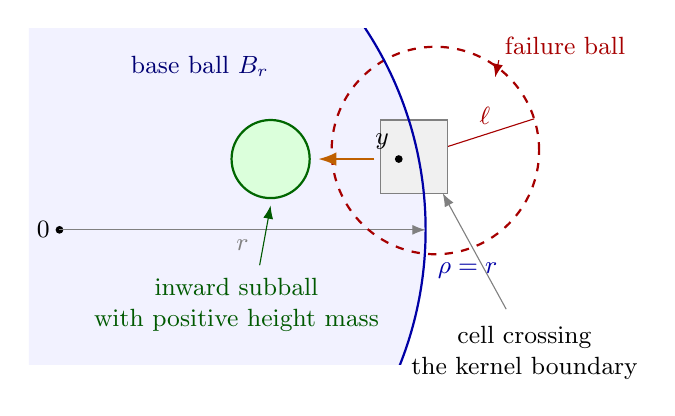
\begin{tikzpicture}[x=1.55cm,y=1.55cm,>=Latex,font=\small]
 \begin{scope}
  \clip (-.25,-1.1) rectangle (4.4,1.65);
  \fill[blue!5] (0,0) circle (3);
 \end{scope}
 \fill (0,0) circle (1.4pt) node[left] {$0$};
 \draw[->,gray] (0,0)--(3,0) node[midway,below] {$r$};
 \node[blue!45!black] at (1.15,1.34) {base ball $B_r$};
 \draw[red!65!black,dashed,thick] (3.08,.65) circle (.85);
 \fill[red!65!black] (3.08,.65) circle (1.4pt);
 \draw[red!65!black] (3.08,.65)--(3.89,.91)
      node[midway,above] {$\ell$};
 \node[red!65!black,anchor=west] at (3.57,1.51) {failure ball};
 \draw[red!65!black,->] (3.6,1.39)--(3.57,1.25);
 \draw[gray,fill=gray!12] (2.63,.3) rectangle (3.18,.9);
 \begin{scope}
  \clip (-.25,-1.1) rectangle (4.4,1.65);
  \draw[blue!65!black,thick] (0,0) circle (3);
 \end{scope}
 \node[blue!65!black,anchor=west] at (3.02,-.33) {$\rho=r$};
 \fill (2.78,.58) circle (1.4pt) node[above left] {$y$};
 \fill[green!14] (1.73,.58) circle (.32);
 \draw[green!40!black,thick] (1.73,.58) circle (.32);
 \draw[->,thick,orange!75!black] (2.58,.58)--(2.12,.58);
 \node[green!35!black,align=center,anchor=north] at (1.45,-.32)
      {inward subball\\with positive height mass};
 \draw[green!35!black,->] (1.64,-.29)--(1.73,.2);
 \node[anchor=north,align=center] at (3.81,-.71)
      {cell crossing\\the kernel boundary};
 \draw[gray,->] (3.66,-.65)--(3.14,.3);
\end{tikzpicture}
\caption{An inward subball controls the boundary weights on the reference center. A failure at
scale $\ell$ supplies separated projection entries on every sufficiently small comparable
subball in its comparison region. Moving such a subball inward by $O(\ell)$
gives positive height mass where the polynomial kernel has a controlled lower
bound. This pays for a local cell even when that cell crosses $\rho=r$. The
picture is schematic; no circular shape of a failure region is assumed.}
\label{fig:collar}
\end{figure}


The separated mass on this inward ball gives
\begin{equation}
 \label{ce:payingheight}
 \delta(r)r\ge c m_0\ell^{k_0}.
\end{equation}
If the support fails to lie on $S$ in every neighborhood, then
$\delta(r)>0$ for every small $r$.  Choose a point with height at
least half the defining supremum.  Its height is nonzero, so it
has a witness as in \eqref{ce:witness}; \eqref{ce:geometry} and
\eqref{ce:payingheight} give
\[
 c m_0\ell^{k_0}\le\delta(r)r
                         \le C m_0\ell^{k_0}.
\]
The inward ball has mass at least $c\ell^m$, height at least
$cm_0\ell^{k_0}$, and $h_r\ge3/4$.  Consequently
\[
 \frac{H(r)}{r^2}
 \ge c\delta(r)^2(\ell/r)^{m+p-1}
 \ge c(m_0)\delta(r)^{2+(m+p-1)/k_0}.
\]
In the last step use
$\ell/r\ge c(m_0)\delta(r)^{1/k_0}r^{1/k_0-1}$ and $r\le1$.
The upper bound in \eqref{ce:height} follows from bounded normalized
mass and $h_r\le1$.  The bound $\delta(r)\le Cr$ follows from
\Cref{ce:center}.  This proves \eqref{ce:height}.

For any point with $t>0$, its witness and
\eqref{ce:payingheight} give
\[
 |H_S|+|\nabla H_S|
 \le Cm_0^2\ell^{2k_0-4}
 \le Cm_0\ell^{k_0-4}\delta(r)r
 \le C\delta(r)r.
\]
At $t=0$ the left side is zero.  This proves
\eqref{ce:pointwisecurvature}.

Finally group points with $t>0$ according to the dyadic scale of
a witnessing failure.  At scale $\ell=2^{-j}$ cover the group by
grid cells of side $c_2\ell$, taking each grid cell only once.
For each occupied cell choose a witness from that group and an
inward ball as above.  On the cell the curvature-square integrand
is at most $Cm_0^4\ell^{4k_0-8}$.  Its mass is at most
$C\ell^m$.  On the corresponding inward ball the integral of
$\phi_r|z|^2$ is at least
$c m_0^2\ell^{2k_0+m}\sup_C\phi_r$ by
\eqref{ce:payingweights}.  Hence
\[
 \int_C\phi_r\bigl(|H_S|^2+|\nabla H_S|^2\bigr)\,\dd\mu
 \le Cm_0^2\ell^{2k_0-8}
                  \int_{B_C}\phi_r|z|^2\,\dd\mu.
\]
The displacement from a cell to its inward ball is $O(\ell)$,
so these balls have bounded overlap at each fixed dyadic scale.
Sum first over the cells and then over $j$.  The geometric series
$\sum_j2^{-j(2k_0-8)}$ converges because $k_0>4$.  Points with
$t=0$ contribute nothing, and division by $r^m$ gives
\eqref{ce:curvature}.
\end{proof}

\begin{corollary}[Regularity when height vanishes]\label{ce:constancy}
If the support lies on the center $S$ in a neighborhood of the origin,
then the origin is regular.
\end{corollary}

\begin{proof}
Write the restricted varifold as $\vartheta\,\HH^m\llcorner S$,
allowing the integer density $\vartheta$ to be zero off its original
support. This is the standard constancy argument; compare
\cite[Chapter~8, Theorem~4.1]{Simon2018}. Tangential first variation gives
$\int_S\vartheta\,\Div_S X=0$ for all compactly supported tangent
fields.  Thus $\vartheta$ is constant almost everywhere on a connected
smaller disk.  The constant is $Q$, by \eqref{ce:typical}.  Normal
first variation gives $H_S=0$, and the small-gradient minimal graph
equation bootstraps $S$ to a smooth graph.  The origin is therefore
regular.
\end{proof}

It remains to exclude the positive-height alternative, which is the
purpose of the inward comparison.

\section{Inward comparison and the conclusion}\label{sec:inward}

We use the center supplied by \Cref{ce:center,ce:weights} at a point
with the density and tangent properties specified there.  If the varifold
lies on the center in a neighborhood of the point, \Cref{ce:constancy}
already gives regularity.  We therefore assume the positive-height
alternative of \Cref{ce:weights} and derive a contradiction.  In particular,
none of the arguments below assumes height doubling at the outset.
The inward subballs in \Cref{ce:weights} controlled the polynomial
weights at each fixed radius.  We now use those bounds in a separate
signed-mass comparison near the same boundary: a radial test handles a
thin outer collar, and the signed-excess theorem applies on interior balls.

\subsection{Signed comparison and frequency identities}

The comparison of height with energy follows Almgren's frequency method
\cite[Section~3.4]{DLS2011}; cutoff frequency on a center manifold is
developed in \cite[Section~3]{DLS2016III}. We derive the identities needed
here from stationarity. The signed-excess estimate supplies the additional
inequality that will yield the inward height comparison.

Keep the physical normal displacement $z$ and the radial functions
\[
 \phi_r=(1-\rho^2/r^2)_+^p,
 \qquad \psi_r=2p(1-\rho^2/r^2)_+^{p-1},
\]
where $p\geq4$ is the fixed integer chosen in \Cref{ce:weights}.
For clarity, write
\[
 \int^{(r)} f\,\dd\nu=r^{-m}\int f\,\dd\nu.
\]
This convention applies both to measures on $S$ and to measures on the
varifold; base functions in a varifold integral are pulled back by nearest
projection.  All integrals below have this normalization unless explicitly
written otherwise.  Abbreviate $\phi_r,\psi_r$ to $\phi,\psi$ at the radius
under consideration.  With $\mathbf u=\nabla_S\rho$, set
\[
 J_z=I-A_z,\qquad K_z=J_z^{-1},\qquad v=K_z\mathbf u,
 \qquad b=B[v,v],\qquad h_r=1-\frac{b}{|v|^2}.
\]
Here $A_z$ is the shape operator in the normal direction $z$; it is
distinct from the scalar $A$ defined next.  Recall that $0\leq h_r\leq1$
and that $h_r$ has no dependence on the radius at a fixed point and tangent
plane.  On the central fiber its value is immaterial, since $z=0$ there.
Define
\begin{equation}\label{in:variables}
 \begin{aligned}
 H&=\int^{(r)}\psi |z|^2h_r\,\dd\mu,
 &A&=r^2\int^{(r)}\phi\,\dd M,\\
 E&=r^2\int^{(r)}\phi\,\dd D,
 &R&=\int^{(r)}\rho^2\psi b\,\dd\mu,\\
 P&=A/H,& n_*&=E/H,\qquad q_*=R/H.
 \end{aligned}
\end{equation}
The scalar ratios $n_*,q_*$ are distinct from the ambient dimension
parameters.  The comparison we need is $2A\leq E$ up to small errors:
after division by $H$, its coefficient one gives $n_*\geq2P$ up to
those errors.  To see its role, omit the errors from the frequency
inequalities proved below.  With a dot denoting differentiation in
$\log r$, their leading terms give, for $P\geq0$,
\[
 q_*\geq n_*^2,\qquad
 \dot P\geq2P-n_*+q_*-2Pn_*
       \geq(n_*-1)(n_*-2P).
\]
Thus the signed comparison makes this leading derivative nonnegative
when $P$ is large.  We first preserve its coefficient through the
boundary of the ball; the bootstrap will then estimate the actual
errors in this calculation.

Put
\[
 \delta=r^{-1}\sup_{\rho<r}|z|,
 \qquad T=\log(r^2/H),\qquad g=T^{-20}.
\]
By \Cref{ce:weights}, after reducing the radius,
\begin{equation}\label{in:smallness}
 0<\delta\leq Cr,\qquad
 c\delta^{J_0}\leq H/r^2\leq C\delta^2,
 \qquad c|\log\delta|\leq T\leq C|\log\delta|.
\end{equation}
The finite exponent $J_0$ and all constants may depend on the fixed center.
We distinguish the unit error $\eta_1(r)=C_1\delta(r)^\alpha$ in the
collar estimate from the common error $\eta(r)=C_\eta\delta(r)^\alpha$
in the frequency argument.  Here $\alpha>0$ is fixed independently of
the multiplier and chosen sufficiently small for the finitely many power errors below, and $C_1$
depends only on the fixed center data.  We choose $C_\eta$ to dominate
the remaining error coefficients and the fixed multiples of $\eta_1$
arising from the actual collar applications.  Their multiplier norms
are verified below to have one bound independent of $r$; no factor
unbounded as $r\downarrow0$ is absorbed into $C_\eta$.  Decreasing
$\alpha$ and increasing the constants a finite number of times gives
common bounds for all the inequalities below.  In particular,
with $s=-\log r$,
\begin{equation}\label{in:exponentialerror}
 T\geq2s-C,\qquad \eta\leq C\exp(-cT).
\end{equation}

The weights first give the following comparisons:
\begin{equation}\label{in:weightcomparison}
 \begin{split}
 \int^{(r)}\phi |z|^2\,\dd\mu
   &\leq C(H+\delta^2E),\\
 \int^{(r)}\psi |z|^2\,\dd\mu
   &\leq C\{H+\delta^2(E+R)\},\\
 r^2\int^{(r)}\phi\,\dd\Lambda
   &\leq Cr^2(H+\delta^2E).
 \end{split}
\end{equation}
Indeed, $\phi\leq C\psi$, $1-h_r\leq Ce$, and $|z|\leq\delta r$
prove the first inequality.  On $\rho<r/2$ the two weights are comparable,
so the same argument applies to the second.  On $r/2\leq\rho<r$ use
$1-h_r\leq Cb$ and $r^2\psi b\leq C\rho^2\psi b$ instead.
The last inequality follows from the weighted curvature estimate in
\Cref{ce:weights} and the definition of $\Lambda$.

\begin{lemma}[The signed estimate up to the outer collar]\label{in:collar}
For $a\in C^1(B_r)$ put
\[
 \|a\|_{1,r}=\sup_{B_r}\bigl(|a|+r|\nabla_Sa|\bigr).
\]
There is a radius $r_{\mathrm c}>0$, depending only on the fixed center
data, such that for every $0<r<r_{\mathrm c}$ the first inequality below
holds for every $a\in C^1(B_r)$ with finite norm, and the second holds
independently of $a$:
\begin{equation}\label{in:collarestimates}
 \begin{split}
 r^2\left|\int^{(r)}a\phi\,\dd M\right|
   &\leq \|a\|_{1,r}\bigl[C(E+r^2H)+\eta_1 R\bigr],\\
 2A&\leq E+Cg(E+H)+Cr^2H+\eta_1 R.
 \end{split}
\end{equation}
The constants $C,C_1$ and the radius $r_{\mathrm c}$ are independent of
the multiplier.  For a family $a_r$, the coefficient of $R$ in the first
line is $\|a_r\|_{1,r}\eta_1(r)$, so each use of its smallness must
control this product.  The second line uses $a=1$ only in its thin-part
proof.
The coefficient of $E$ in the second line is exactly one before the
displayed small errors are added.
\end{lemma}

\begin{proof}
For the absolute estimate it suffices to treat $\|a\|_{1,r}\leq1$
uniformly: apply that case to $a/\|a\|_{1,r}$ when the norm is positive,
and the zero case is immediate.  The signed estimate will use the member
$a=1$ of this unit class.
Choose a small fixed $\beta>0$, with $\beta<1/4$, and put
$\sigma=\delta^\beta$; we may take $0<\alpha\leq2\beta$ in $\eta_1$.
Choose a radial cutoff $\chi$ equal to one
when $0\leq1-\rho/r\leq\sigma^2$, equal to zero when
$1-\rho/r\geq2\sigma^2$, and with derivative bounded by
$C/(\sigma^2r)$.  Write $\phi_{\rm thin}=\chi\phi$ and
$\phi_{\rm bulk}=(1-\chi)\phi$.

We first treat the bulk, including the overlap with the thin part.
Fix first an enlargement factor $c_{\mathrm{out}}>8$ sufficient for
\Cref{lt:scalar,sx:signed} and for a Caccioppoli cutoff equal to one on
$B_{8\ell}$ and supported in $B_{c_{\mathrm{out}}\ell}$.  Then choose
the fixed $c_0$ small and put $\ell=c_0\sigma^2r$.  Cover the bulk by
balls of radius $\ell$ with centers $x_i$ in its support.  These centers
have boundary depth at least $\sigma^2r$, so $c_0$ can be chosen so that
all $B_{c_{\mathrm{out}}\ell}(x_i)$ stay inside $B_r$.  Choose the cover
with bounded overlap of these enlargements and so that the intermediate
balls on which \Cref{lt:scalar} selects integers have overlaps of fixed
positive relative volume along the connecting chains.  Choose a smooth
nonnegative partition of unity $\{\vartheta_i\}$ subordinate to the
original balls, with
\[
 |D^j\vartheta_i|\leq C_j\ell^{-j}\qquad(0\leq j\leq k),
\]
where $D$ denotes base-coordinate derivatives and $k=k(m)$ is the finite
test order in \Cref{lt:potential}.  Put $\phi_i=\phi(x_i)$.  On each
enlargement $\phi$ is comparable to $\phi_i$.  The partitioned
weights, divided by $\phi_i$ and by a fixed constant,
have Lipschitz norm at most one in units of $\ell$.

The mass on each enlarged ball is at most $C\ell^m$.  To see this
without assuming a local graphical representation, observe that
$\delta r=o(\ell)$; thus the part of the tube over the ball lies in an
ambient ball of radius $C\ell$ centered at a support point.  The upper
bound follows by monotonicity, comparing with an ambient ball of radius
comparable to $r$ and using the fixed normalized mass bound at the
origin.  Empty balls need no estimate.

For the local tilt estimate, use ordinary, unnormalized physical
integrals.  Let $\xi$ be a base cutoff equal to one on $B_{4\ell}$,
supported in $B_{c_{\mathrm{out}}\ell}$, and satisfying
$|\nabla_S\xi|\leq C/\ell$.  The analogous cutoff equal to one on
$B_{8\ell}$ has the same derivative bound and outer support.
Testing stationarity with $\xi^2z$
and using the normal-displacement trace \eqref{ce:normaltrace} gives
\[
 \int\xi^2e\,\dd\mu
 \leq C\int\left[
   \bigl(|\nabla_S\xi|^2+|\mathrm{II}|^2\xi^2\bigr)|z|^2
          +\xi^2|H_S||z|\right]\,\dd\mu.
\]
Indeed, the derivative of the cutoff contributes at most
$C\xi|\nabla_S\xi||z|\sqrt e$; Young's inequality absorbs this term
and the small $|\mathrm{II}||z|e$ term from the trace.  The displayed
$|H_S||z|$ term is retained because the center need not be minimal.
The bounds $|z|\leq\delta r$ and
$|H_S|+|\nabla H_S|\leq C\delta r$, together with the local mass
bound, give
$\ell^{-m}D(B_{4\ell})\leq C[(\delta r/\ell)^2+(\delta r)^2]$.
The definition of $\Lambda$ gives
$\ell^{-m}\Lambda(B_{4\ell})\leq C(\delta r)^2$ separately.  Hence
\begin{equation}\label{in:localdensity}
 \ell^{-m}(D+\Lambda)(B_{4\ell})
       \leq C(\delta/\sigma^2)^2
       \leq C\delta^{2-4\beta}.
\end{equation}
The same estimate holds on $B_{8\ell}$, using its cutoff in
$B_{c_{\mathrm{out}}\ell}$.  These enlargement factors were fixed
before $c_0$.
The coordinates have the required fixed geometry bounds, and the terms
in $\Lambda$ still use physical units.

Apply \Cref{lt:scalar} first to select the local integers.  On the
intermediate balls just chosen, the scalar exceptional sets have relative
volume $O(\delta^{2-4\beta})$.  For small $r$ they cannot fill the
chosen overlaps of fixed positive relative volume, so their integers
agree.  The bulk is connected; call
the common integer $q_r$.  To identify it, rescale one fixed smooth
nonnegative test supported in $B_{1/2}$ to $B_{r/2}$ and normalize
its reference-volume integral to one.  Call it $\varphi_r$; then
$|D^j\varphi_r|\leq Cr^{-m-j}$ for $0\leq j\leq k$.  Partition this test
over the cover.  After pullback to a unit $\ell$-cell, each product
$\vartheta_i\varphi_r$ has $C^k$ norm at most $Cr^{-m}$, since
$\ell\leq r$.  The coordinate-volume factor in the scalar proof has
fixed scaled derivative bounds through order $k$, so multiplying by it
preserves this estimate.  The distributional estimate
\eqref{eq:lt-distribution-control} used in the proof of \Cref{lt:scalar}, with
\eqref{in:localdensity}, bounds each cell's error relative to $q_r$ by
$C\delta^{2-4\beta}\ell^m r^{-m}$.  Bounded overlap gives
$\sum_i\ell^m\leq Cr^m$, so its projected-mass average differs from
$q_r$ by at most $C\delta^{2-4\beta}$.  Tangent convergence and
the smooth rescaling of the fixed center make that same average
$Q+o(1)$.  Integrality therefore gives $q_r=Q$ for all sufficiently
small $r$.  Exact agreement on overlaps involves no error accumulated
along the chain of balls.  This also identifies the integer on the
balls used in the overlap and in the thicker error collar below.
Consequently \Cref{lt:scalar} bounds $|M|$ on each smaller ball by the
enlarged $D+\Lambda$ mass.  In particular, applying it with fixed
interior room and using \eqref{in:localdensity} also on the larger
ball gives
\begin{equation}\label{in:localscalar}
 \begin{split}
 |M|(B_{4\ell}(x_i))
   &\leq C(D+\Lambda)(B_{8\ell}(x_i)),\\
 \ell^{-m}\tau(B_{4\ell}(x_i))
   &\leq C\delta^{2-4\beta}.
 \end{split}
\end{equation}
All these balls lie inside $B_r$ by the choice of $c_0$.
Summation with comparable weights gives
\begin{equation}\label{in:bulkvariation}
 r^2\int^{(r)}\phi_{\rm bulk}\,\dd|M|
       \leq Cr^2\int^{(r)}\phi\,\dd(D+\Lambda)
       \leq C(E+r^2H),
\end{equation}
using \eqref{in:weightcomparison} to absorb a small multiple of $E$.
For every member of the unit multiplier class this also gives
$r^2|\int^{(r)}a\phi_{\rm bulk}\,\dd M|\leq C(E+r^2H)$.

For the signed estimate, invoke \Cref{sx:signed} afresh on each normal
chart at physical radius $\ell$.  The measures $M,D,\Lambda$ and the
base tests are geometric, so they give the required data in the unit
coordinates, with the measures divided by $\ell^m$.  The physical
condition below belongs to this new theorem instance; it does not change
the inherited geometry parameter in an off-center rescaling of a prior
instance.  On a cell use
\[
 d_i=\max\{C\ell^{-m}\tau(B_{4\ell}(x_i)),\ \delta^{2J_0+4}\},
 \qquad T_i=-\log d_i,
\]
with the fixed enlargement and constant sufficient for
\Cref{sx:signed}.  Equation \eqref{in:localscalar} shows that
$c|\log\delta|\leq T_i\leq(2J_0+4)|\log\delta|$, where the upper
bound follows from the floor in $d_i$.  Moreover
\[
 \ell+\sup|z|\leq C\delta^{2\beta}
                       \leq \exp(-\kappa T_i)
\]
for some fixed $\kappa>0$ and all small $r$; choose, for example,
$\kappa(2J_0+4)<2\beta$.  Thus both smallness hypotheses of
\Cref{sx:signed} hold even if $\delta$ is smaller than every fixed
power of $r$.

Apply that result to
$w_i=\vartheta_i\phi_{\rm bulk}/(C\phi_i)$ in the coordinates scaled
by $\ell$.  They are supported in $B_1$ in those coordinates and satisfy
$0\leq w_i\leq1$ and $\Lip w_i\leq1$.  Restoring
the physical measure factor $\ell^m$ and then the normalization
$r^{2-m}$ gives
\begin{equation}\label{in:bulksigned}
 \begin{split}
 2r^2\int^{(r)}\phi_{\rm bulk}\,\dd M
 &\leq r^2\int^{(r)}\phi_{\rm bulk}\,\dd D
       +C_Q r^2\int^{(r)}\phi_{\rm bulk}\,\dd\Lambda\\
 &\quad+C r^{2-m}\sum_i\phi_i\ell^m d_i e^{-F_Q(T_i)}.
 \end{split}
\end{equation}
The last sum includes the enlarged cells, even where
$\phi_{\rm bulk}$ vanishes in the overlap with the thin part.
On these cells use the local estimate \eqref{in:localscalar}:
$\phi$ is comparable to $\phi_i$ throughout $B_{8\ell}(x_i)$, and
these balls have bounded overlap inside $B_r$.  Therefore
\[
 \begin{split}
 \sum_i\phi_i\ell^m d_i
 &\leq C\sum_i\phi_i\tau(B_{4\ell}(x_i))
                  +C\delta^{2J_0+4}\sum_i\phi_i\ell^m\\
 &\leq C\sum_i\phi_i(D+\Lambda)(B_{8\ell}(x_i))
                  +C\delta^{2J_0+4}\sum_i\phi_i\ell^m\\
 &\leq Cr^m\int^{(r)}\phi\,\dd(D+\Lambda)
                  +Cr^m\delta^{2J_0+4}.
 \end{split}
\]
Here the last floor sum is bounded by the ordinary volume of the
bounded-overlap cover.  Since $T_i\geq c|\log\delta|$ and
$\exp[-F_Q(c|\log\delta|)]$ is smaller than any fixed negative power
of $T$, the remainder in \eqref{in:bulksigned} is at most
\[
 Cg\left(r^2\int^{(r)}\phi\,\dd(D+\Lambda)
                      +r^2\delta^{2J_0+4}\right).
\]
The floor term $r^2\delta^{2J_0+4}$ is at most
$C\delta^{J_0+4}H$ by \eqref{in:smallness}.  The weighted comparison
\eqref{in:weightcomparison} controls the remaining integral by
$C(E+r^2H)$ and bounds the $C_Q\Lambda$ term in
\eqref{in:bulksigned} by $Cr^2H+o(g)E$, since $r^2\delta^2=o(g)$.
This proves the second line
of \eqref{in:collarestimates} for the bulk, with its leading tilt term
unchanged.

It remains to estimate the signed mass on the thin part.  A direct
total-variation estimate here would unnecessarily add a full-tilt
term.  Instead solve a radial divergence equation.  In geodesic polar
coordinates write the volume element as $j(\rho,\omega)\,\dd\rho\,
\dd\omega$.  Throughout this thin calculation $\|a\|_{1,r}\leq1$,
and all constants are uniform over that class.  Initially put
\[
 F(\rho,\omega)=-j(\rho,\omega)^{-1}
       \int_\rho^r a(t,\omega)\phi_{\rm thin}(t)
                              j(t,\omega)\,\dd t,
 \qquad X=F\mathbf u.
\]
Then $\Div_S X=a\phi_{\rm thin}$.  Multiply $X$ by a radial cutoff
equal to one at depths $r-\rho\leq\sigma r$ and zero at depths
$r-\rho\geq2\sigma r$.  On this latter collar the integrated numerator
has size $O(r\sigma^{2p+2})$ relative to $j$.  The cutoff divergence
error $q_c$ consequently satisfies
\[
 \Div_S X=a\phi_{\rm thin}+q_c,
 \qquad |q_c|\leq C\sigma^{p+1}\phi,
\]
and is supported where $\sigma r\leq r-\rho\leq2\sigma r$.
The same integration, also differentiated in angular directions, gives
\begin{equation}\label{in:radialfield}
 |X|/r+
 |\nabla_SX-a\phi_{\rm thin}\mathbf u\otimes\mathbf u|
       \leq C\sigma^2\phi.
\end{equation}
For example, at depth $d r\leq2\sigma^2r$ the primitive divided by
$r$ is $O(d^{p+1})$, whereas $\phi\asymp d^p$; beyond that depth its
size is $O(\sigma^{2p+2})$.  On the cutoff collar the derivative loss
$\sigma^{-1}$ still leaves $\sigma^{p+1}\phi$.
This proves \eqref{in:radialfield}; bounded derivatives of the polar
volume factor only change its constants.  A radial spatial derivative
of the primitive uses the value of $a$ at its lower endpoint; an angular
derivative uses only its first spatial derivative, bounded by $1/r$.
The scale parameter $r$ is held fixed in this calculation.  Near
$\rho=r$, the preceding estimates give $|F|\leq Crd^{p+1}$ and
$|\nabla_S(F\mathbf u)|\leq Cd^p$.  Thus $X$ and its first derivative
vanish at the boundary, so extending $X$ by zero gives a $C^1$ compactly
supported base field using only values of $a$ in $B_r$.  The inner cutoff
removes the polar origin.  When $m=1$ the construction is made separately
on the two radial intervals and has no angular term.

Use the lifted field of \Cref{lt:curvedvariation}.  The $q_cM$ term
is estimated by the already proved bulk total-variation bound: for small
$\sigma$, its support has depth between $\sigma r$ and $2\sigma r$, where
$\chi=0$ and $\phi_{\rm bulk}=\phi$.  Its contribution is at most
$C\sigma^{p+1}(E+r^2H)$.  Put
$W=\int^{(r)}\phi|z|^2\,\dd\mu\leq C(H+\delta^2E)$.
Equation \eqref{in:radialfield} gives $|X|\leq C\sigma^2r\phi$ and
$|\nabla_SX|\leq C\phi$.  After multiplication by $r^2$, the three
error types in \Cref{lt:curvedvariation} are therefore bounded by
\[
 C\delta rE,\qquad C\sigma^2r^3W,\qquad
 C\sigma^2r^2\sqrt{EW},
\]
using the weighted curvature-square bound for the term containing
$\nabla^\perp H_S$.  Young's inequality puts these terms into
$Cr^2H+C(\delta r+\sigma^2)E$.  The stress left after its radial part
costs $C\sigma^2E$.  Since $p\geq4$, $r\leq1$, and
$0<\alpha\leq2\beta$, all these small coefficients of $E$ are at most
$\eta_1$ after fixing $C_1$.  The main stress term gives
\begin{equation}\label{in:thinmass}
 r^2\left|\int^{(r)}a\phi_{\rm thin}\,\dd M\right|
 \leq Cr^2\int^{(r)}\phi_{\rm thin}B[\mathbf u,\mathbf u]\,\dd\mu
                  +\eta_1 E+Cr^2H.
\end{equation}
Since $\rho\geq r/2$ on the thin part,
\[
 \phi_{\rm thin}\leq C\sigma^2(\rho/r)^2\psi,
 \qquad B[\mathbf u,\mathbf u]\leq2b+C|z|^2e.
\]
Thus the first term of \eqref{in:thinmass} is at most
$C\sigma^2R+C\delta^2r^2E\leq\eta_1(R+E)$, after increasing $C_1$.
Adding the unit bulk bound gives
\[
 r^2\left|\int^{(r)}a\phi\,\dd M\right|
 \leq C(E+r^2H)+\eta_1R\qquad(\|a\|_{1,r}\leq1).
\]
Homogeneity now gives the first line of \eqref{in:collarestimates} on
the same radius interval.  For the signed estimate use $a=1$, add twice
its thin-part bound to the bulk signed estimate, and use
$\int\phi_{\rm bulk}\,\dd D\leq\int\phi\,\dd D$.
Because $\eta_1=o(g)$ by \eqref{in:smallness}, its $E$ term is absorbed
into $CgE$ after reducing the fixed radius.  Enlarge $C_1$ once to cover
the fixed factors in both conclusions.  The coefficient one has
been preserved as claimed.
\end{proof}

\begin{lemma}[Frequency inequalities]\label{in:frequency}
With a dot denoting differentiation with respect to $\log r$, the
quantities in \eqref{in:variables} satisfy
\begin{align}
 n_*&\leq\sqrt{q_*}+Cr^2+\eta n_*,\label{in:normalfrequency}\\
 \left|\frac{\dot A}{H}-(2P-n_*+q_*)\right|
  &\leq C\{r\sqrt{q_*}+r^2(1+n_*)\}+\eta(n_*+q_*),
                         \label{in:horizontalfrequency}\\
 -m\leq\frac{\dot H}{H}
  &\leq2n_*+Cr+\eta(n_*+q_*).\label{in:heightfrequency}
\end{align}
\end{lemma}

\begin{proof}
Test normal stationarity with $z\phi$.  The exact normal-displacement trace formula
\eqref{ce:normaltrace} and \eqref{in:weightcomparison} give
\begin{equation}\label{in:normalflux}
 \left|E-\int^{(r)}\rho\psi
                     z\cdot P_{vh}v\,\dd\mu\right|
       \leq Cr^2H+\eta E.
\end{equation}
In particular the $H_S\cdot z$ term is bounded using the weighted
curvature-square estimate, rather than a height-independent error.
For the tangent projection $P_T$, the algebra is exact: $P_T^2=P_T$
and $(P_T)_{hh}=I-B$
imply
\[
 |P_{vh}v|^2=v\cdot(B-B^2)v
       =b-|Bv|^2
       \leq b-\frac{b^2}{|v|^2}=bh_r.
\]
Cauchy--Schwarz therefore bounds the absolute value of the flux in
\eqref{in:normalflux} by $\sqrt{RH}$.  Division by $H$ proves
\eqref{in:normalfrequency}.

For the horizontal identity put $Z_0=\rho\mathbf u$ on $S$ and let
$\overline Z_0(q)=J_zZ_0(\pi q)$ be its unweighted lift.  We first
compute the full derivative of the kernel in the test
$(\phi\circ\pi)\overline Z_0$.  Since $D\pi=K_zP_h$ and
$\nabla_S\phi=-(\rho/r^2)\psi\mathbf u$,
\[
 \nabla(\phi\circ\pi)=-\frac{\rho}{r^2}\psi K_z\mathbf u.
\]
Both this vector and $\overline Z_0=\rho J_z\mathbf u$ are horizontal.
The product rule and $(P_T)_{hh}=I-B$ therefore give exactly
\[
 \begin{split}
 P_T:D\bigl((\phi\circ\pi)\overline Z_0\bigr)
 &=\phi P_T:D\overline Z_0
   -\frac{\rho^2}{r^2}\psi
       (K_z\mathbf u)\cdot(I-B)(J_z\mathbf u)\\
 &=\phi P_T:D\overline Z_0-\frac{\rho^2}{r^2}\psi
   +\frac{\rho^2}{r^2}\psi B[K_z\mathbf u,J_z\mathbf u].
 \end{split}
\]
The identity coefficient is one because $J_z,K_z$ are self-adjoint
inverses and $(K_z\mathbf u)\cdot(J_z\mathbf u)=|\mathbf u|^2=1$.
The radial terms are understood to be zero on the central fiber, as
their factors of $\rho^2$ require.

For the remaining derivative, the pointwise block calculation in the
proof of \Cref{lt:curvedvariation} gives
\[
 \begin{split}
 P_T:D\overline Z_0
 &=\Div_SZ_0-B:\nabla_SZ_0+\varepsilon_Z,\\
 |\varepsilon_Z|
 &\leq C\left\{|z|e|\nabla_SZ_0|
  +\left[(|\nabla^\perp H_S|+|z|)|z|+\sqrt e\,|z|\right]|Z_0|\right\}.
 \end{split}
\]
This is the estimate for the unweighted lift, so the product formula
multiplies its entire remainder by $\phi$.  Subtract the reference
identity $Q\int_S\Div_S(\phi Z_0)\,\dd\vol_S=0$, in which
$\Div_S(\phi Z_0)=\phi\Div_SZ_0-\rho^2\psi/r^2$.  Since
$\dot A=(2-m)A+\int^{(r)}\rho^2\psi\,\dd M$, we obtain, with
\[
 \widetilde R=\int^{(r)}\rho^2\psi
                  B[K_z\mathbf u,J_z\mathbf u]\,\dd\mu,
\]
the exact identity
\begin{equation}\label{in:horizontalidentity}
 \begin{split}
 \dot A={}&2A-E+\widetilde R
   +r^2\int^{(r)}\phi(\Div_SZ_0-m)\,\dd M\\
 &-r^2\int^{(r)}\phi B:(\nabla_SZ_0-I)\,\dd\mu
   +r^2\int^{(r)}\phi\varepsilon_Z\,\dd\mu.
 \end{split}
\end{equation}

In geodesic normal coordinates $y$, Gauss' lemma gives
$Z_0=y^i\partial_i$.  If $g^S_{ij}$ are the metric components, then
\[
 f:=\Div_SZ_0-m=y\cdot D\log\sqrt{\det(g^S_{ij})}.
\]
The logarithmic volume factor has vanishing first derivative at $0$
and bounded second derivative in the fixed chart.  Consequently
\[
 |f|\leq C\rho^2,\qquad |\nabla_Sf|\leq C\rho,
 \qquad \|a_r\|_{1,r}\leq K_{\mathrm{geo}},\quad a_r=f/r^2,
\]
for one fixed $K_{\mathrm{geo}}$.  Also
$\nabla_SZ_0=I+O(\rho^2)$.  The number
$K_{\mathrm{app}}=\max\{1,K_{\mathrm{geo}}\}$ bounds both actual
collar multipliers: $a_r$ here and $a=1$ in the bootstrap.  Choose
$C_\eta$ in the convention above to dominate $K_{\mathrm{app}}C_1$
and the finitely many other error prefactors in the frequency estimates.
Then $\eta\geq K_{\mathrm{app}}\eta_1$ has a fixed prefactor, so
\eqref{in:exponentialerror} applies.  The first line of
\eqref{in:collarestimates} and positivity of $B$ now give
\[
 \begin{split}
 r^2\left|\int^{(r)}\phi(\Div_SZ_0-m)\,\dd M\right|
   &\leq Cr^2(E+r^2H)+r^2\eta R,\\
 r^2\left|\int^{(r)}\phi B:(\nabla_SZ_0-I)\,\dd\mu\right|
   &\leq Cr^2E.
 \end{split}
\]
For the pointwise remainder use $|Z_0|\leq r$,
$|\nabla_SZ_0|\leq C$, and $\sup|z|\leq\delta r$.  The first
and last lines of \eqref{in:weightcomparison}, followed by
Cauchy--Schwarz, bound its three terms respectively by
\[
 \begin{split}
 r^2\int^{(r)}\phi|\varepsilon_Z|\,\dd\mu
 &\leq C\delta rE+Cr^3(H+\delta^2E)
                  +Cr^2\sqrt{E(H+\delta^2E)}\\
 &\leq Cr^2(E+H)+\eta E.
 \end{split}
\]
Here the term involving $\nabla^\perp H_S$ uses the weighted
curvature-square bound inside $\Lambda$; the last term comes from
$\sqrt e\,|z|\,|Z_0|$.

It remains to compare the radial stress $\widetilde R$ with $R$.
Positivity of $B$, its trace $e$, and $|J_z-K_z|\leq C|z|$ imply
$|B[v,(J_z-K_z)\mathbf u]|\leq C|z|\sqrt{be}$.  Thus
$|\widetilde R-R|$ is at most
\begin{equation}\label{in:radialreplacement}
 Cr\sqrt R\left(\int^{(r)}\psi|z|^2e\,\dd\mu\right)^{1/2},
\end{equation}
by Cauchy--Schwarz.  Since $e\leq m$, the second line of
\eqref{in:weightcomparison} gives
\[
 |\widetilde R-R|
 \leq Cr\sqrt{RH}+C\delta r\sqrt{R(E+R)}
 \leq Cr\sqrt{RH}+\eta(E+R).
\]
Combining these estimates in \eqref{in:horizontalidentity} and dividing
by $H$ proves \eqref{in:horizontalfrequency}.  The differentiated
kernel has been exhausted by $\widetilde R$; every other remainder in
that identity carries the weight $\phi$.

Finally, set
\[
 Y=\frac{\rho K_z\mathbf u}{|K_z\mathbf u|^2}.
\]
This field is defined independently of the varifold tangent plane.
Since $\nabla\rho=K_z\mathbf u$, it satisfies
$Y\cdot\nabla_T\rho=\rho h_r$.  Testing stationarity with
$\psi|z|^2Y$ consequently cancels the differentiated kernel exactly
and gives
\begin{equation}\label{in:heightidentity}
 \dot H=\int^{(r)}\psi\left\{
 |z|^2(\tr_T DY-mh_r)
 +\frac{2\rho z\cdot P_{vh}K_z\mathbf u}{|K_z\mathbf u|^2}
                         \right\}\,\dd\mu.
\end{equation}
There is no derivative of the measurable tangent projection in this
calculation.  Also $\nabla|z|^2=2z$ in the ambient Euclidean space,
so normal-frame connection terms do not arise from this factor.

The center estimates give $t(y)=o(\rho(y))$ and hence
$|z|\leq C\rho^2$ on the support near the origin.  Although
derivatives of $\mathbf u$ have size $O(\rho^{-1})$, differentiation
of $Y$ thus gives, on the support,
\[
 DY=P_h+O(\rho+|z|/\rho)=P_h+O(r).
\]
It follows that $\tr_TDY-mh_r=m(1-h_r)-e+O(r)$.
The positive $m(1-h_r)$ contribution is bounded by
$C\delta^2(E+R)$, by the proof of \eqref{in:weightcomparison}.
The $O(r)$ contribution is at most $CrH+\eta(E+R)$, and the term
$-e|z|^2$ can be discarded for an upper bound.  Replacing the
denominator in the second term of \eqref{in:heightidentity} by one
costs at most $C\delta r\sqrt{RH}\leq CrH+\eta R$.
Equation \eqref{in:normalflux} now proves the upper bound in
\eqref{in:heightfrequency}.

To justify the test at the central fiber, first remove $\rho<\epsilon$
by a smooth radial cutoff $\chi_\epsilon$, equal to zero for
$\rho\leq\epsilon$, equal to one for $\rho\geq2\epsilon$, and satisfying
$|\nabla\chi_\epsilon|\leq C/\epsilon$.  Since $|Y|\leq C\rho$,
$|Y||\nabla\chi_\epsilon|\leq C$ on the transition annulus.  Its extra
term is therefore bounded, at fixed $r$, by a constant times
$r^{-m}\int_{\rho<2\epsilon}|z|^2\,\dd\mu$, which tends to zero.
The preceding support bound and local mass bounds also justify all
other limiting terms.  The lower bound in
\eqref{in:heightfrequency} follows directly from differentiating
$r^{-m}\psi_r$: its derivative in $\log r$ is at least
$-m r^{-m}\psi_r$, and the remaining factor $|z|^2h_r$ is
nonnegative and independent of $r$.
\end{proof}

\subsection{Doubling and vanishing height}

\begin{proposition}[The inward bootstrap]\label{in:bootstrap}
On all sufficiently small radii, $P$ is bounded above and below.
For each fixed $\lambda\in(0,1)$ there are constants $C_\lambda,c_\lambda>0$
such that
\begin{equation}\label{in:doubling}
 c_\lambda H(r)\leq H(\lambda r)\leq C_\lambda H(r),
 \qquad
 \int_{\lambda r}^{r}q_*(v)\,\frac{\dd v}{v}\leq C_\lambda.
\end{equation}
There is a sequence $r_j\downarrow0$ on which both $n_*(r_j)$ and
$q_*(r_j)$ are bounded.
\end{proposition}

\begin{proof}
All quantities are locally absolutely continuous as functions of
$\log r$ where differentiated; $H>0$, and inequalities for derivatives
may be read almost everywhere.  Put
$v_0=\dot A/H$ and $h_0=\dot H/H$ temporarily.  The first line of
\eqref{in:collarestimates} with $a=1$, followed by
\eqref{in:normalfrequency}, gives
\[
 |P|\leq C(n_*+r^2)+\eta q_*
       \leq C(\sqrt{q_*}+r^2)+C\eta q_*.
\]
It follows, for a sufficiently large fixed $K$ and $|P|\geq K$, that
\begin{equation}\label{in:largefrequency}
 \frac{q_*}{|P|}\geq c\min\{|P|,\eta^{-1}\},
 \qquad v_0\geq cq_*.
\end{equation}
For the first assertion, either $C\sqrt{q_*}$ or $C\eta q_*$ is at least
a fixed fraction of $|P|$.  The second follows from
\eqref{in:horizontalfrequency}, increasing $K$ and then shrinking the
radius so that $q_*$ absorbs $2|P|$, $n_*$, and every error.

If $P\leq-K$, the lower bound $h_0\geq-m$ gives
\[
 \dot P=v_0-Ph_0\geq cq_*+mP>0.
\]
Such an excursion persists as the radius decreases: in inward time
$s=-\log r$, $P_s<0$ throughout this region.  There also $A<0$ and
$\dot A>0$, so $A$ decreases inward and stays below a fixed negative
number.  This contradicts $A\to0$, which follows from its factor
$r^2$ and bounded normalized mass.  We conclude that $P\geq-K$ on
the small-radius interval.

There are arbitrarily small radii at which $P\leq T^2$.  Otherwise,
eventually $P>T^2$, and \eqref{in:largefrequency} and
\eqref{in:exponentialerror} imply $v_0/P\geq cT^2$.  Define
\[
 Z=\log(r^2/A)=T-\log P.
\]
Inward differentiation gives $Z_s=v_0/P-2\geq cT^2-2$.
Since $T\geq2s-C$, $Z$ becomes positive and unbounded.  Also $Z\leq T$
in this regime, whence eventually $Z_s\geq c'Z^2$.
Integrating $(1/Z)_s\leq-c'$ forces a blow-up at finite inward time,
although $A,H$ are defined and positive throughout every finite
subinterval of this regime.  This is impossible.

We next prove the differential estimate
\begin{equation}\label{in:moderatefrequency}
 \dot P\geq-C(rP+gP^2)
                \qquad\hbox{when }K\leq P\leq T^4.
\end{equation}
Combining \eqref{in:horizontalfrequency} and
\eqref{in:heightfrequency} gives
\[
 \dot P\geq 2P-n_*+q_*-2Pn_*
 -C\{r\sqrt{q_*}+r^2(1+n_*)+rP\}
 -C\eta(1+P)(n_*+q_*).
\]
If $q_*\geq L P^2$ for a sufficiently large fixed $L$, then
$n_*\leq C\sqrt{q_*}+Cr^2$ and $\eta T^4=o(1)$ show that the right-hand
side is positive.  Otherwise $n_*\leq CP$, and squaring
\eqref{in:normalfrequency} gives
\[
 q_*\geq n_*^2-Cr^2P-C\eta P^2.
\]
The independent signed second line of \eqref{in:collarestimates}, with
$\eta_1\leq\eta$, gives
\[
 n_*\geq2P-d_0,\qquad
 d_0=C(gP+r^2+\eta P^2).
\]
For large $K$ and small $r$, this also gives $n_*>1$.  The principal
terms factor as
\[
 2P-n_*+n_*^2-2Pn_*=(n_*-1)(n_*-2P)\geq-CPd_0.
\]
Thus $\dot P\geq-C(rP+gP^2+\eta P^3)$.  The last term is absorbed
by $gP^2$, since $P\leq T^4$ and
$\eta T^4\leq g$ after shrinking the radius.  This proves
\eqref{in:moderatefrequency}.

It remains to justify that this restricted estimate gives a bound on
every smaller radius.  Choose an arbitrarily small moderate radius
$r_0=e^{-s_0}$, so $P_0\leq T_0^2$.  Take $s_0$ so large that
\[
 \int_{s_0}^{\infty}C\{e^{-s}+T(s)^{-16}\}\,\dd s
       \leq\varepsilon_0<1.
\]
This is possible by \eqref{in:exponentialerror}.  On each component
where $P\geq K$, before a possible exit through $P=T^4$,
\eqref{in:moderatefrequency} yields
\[
 (\log P)_s\leq C(r+gP)\leq C(r+T^{-16}).
\]
Moreover $Z_s>0$ there by \eqref{in:largefrequency}, increasing $K$
if necessary.  If the first component starts at $s_0$, these inequalities
give
\[
 P\leq e^{\varepsilon_0}P_0\leq e^{\varepsilon_0}T_0^2,
 \qquad
 T=Z+\log P\geq T_0-\log P_0+\log K\geq T_0/2.
\]
For large $T_0$ these bounds exclude $P=T^4$.  If a component starts
later, at $s_i$, then $P(s_i)=K$, and the same argument gives
$P\leq e^{\varepsilon_0}K$ and $T\geq T(s_i)$ there, again excluding
the upper exit.  This proves the finite uniform bound
\[
 -K\leq P(r)\leq e^{\varepsilon_0}\max\{K,P_0\}
                     \qquad(0<r\leq r_0).
\]

Write this bound as $|P|\leq B_0$.  After $B_0$ is fixed, choose
$0<\bar r_0\leq r_0$ so that $C\eta(1+B_0)\leq1/4$ for the constants in
\Cref{in:frequency} whenever $0<r\leq\bar r_0$; this absorbs its
$\eta q_*$ terms after quotient differentiation.  For $P\geq0$ use the
upper height derivative bound in $\dot P=v_0-Ph_0$; for $P<0$ use its
lower bound.  In both cases \Cref{in:frequency} and
$n_*\leq C\sqrt{q_*}+Cr^2$ imply
\begin{equation}\label{in:integralenergy}
 \dot P\geq cq_*-C_{B_0}.
\end{equation}
Integrating over a logarithmic interval of fixed length bounds
$\int q_*\,\dd\log r$.  Cauchy--Schwarz then bounds
$\int n_*\,\dd\log r$, and integration of
\eqref{in:heightfrequency} proves both sides of the height comparison
in \eqref{in:doubling}.  In each interval
$[2^{-j-1}\bar r_0,2^{-j}\bar r_0]$ choose a radius where $q_*$ is
bounded by its logarithmic average.  Equation \eqref{in:normalfrequency}
bounds $n_*$ at those radii, proving the last assertion.
\end{proof}

\begin{proposition}[Vanishing height at a typical point]\label{in:finish}
The positive-height alternative at the origin is impossible.
Consequently every point satisfying the typical-point hypotheses \eqref{ce:typical} is regular.
\end{proposition}

\begin{proof}
Take the radii $r_j$ from \Cref{in:bootstrap}, and write $r=r_j$.
On $\rho<3r/4$ the weights $\phi,\psi$ have positive lower bounds
depending only on $p$.  Equations \eqref{in:weightcomparison},
\eqref{in:normalfrequency}, and the boundedness of $n_*,q_*$ give
\begin{equation}\label{in:selectedenergy}
 r^{-m}\int_{\rho<3r/4}|z|^2\,\dd\mu
       +r^{2-m}(D+\Lambda)(B_{3r/4})\leq CH(r).
\end{equation}
Here a height integral is over the part of the separated tube above
the indicated base ball, whereas $D,\Lambda$ are projected measures.
On the other hand, applying \eqref{in:doubling} with $\lambda=1/4$
and using $\psi\leq2p$, $h_r\leq1$ at radius $r/4$ gives
\begin{equation}\label{in:heightlower}
 r^{-m}\int_{\rho<r/4}|z|^2\,\dd\mu\geq cH(r)>0.
\end{equation}

Fix an exceptional fraction $\delta_{\mathrm{cfg}}=1/4$ and a finite
exponent $p_*>2$ satisfying $m(1/2-1/p_*)<1$.  Use the enlargement $c$
fixed from the local data in \Cref{lt:config}, with the required
scalar-selection room, and then fix
$d_{\mathrm{cfg},0}=d_0(\delta_{\mathrm{cfg}})>0$.  Then choose
$\epsilon>0$ so small that $B_{r/4}$ has a finite cover by balls of
radius $\epsilon r$ whose required enlargements lie in $B_{r/2}$.
The number of balls and $\epsilon$ are fixed independently of $r$.

Apply \Cref{lt:scalar} with room between $3r/4$ and $r/2$; its
integer is again $Q$.  Its variation estimate and
\eqref{in:selectedenergy} give, for every enlarged ball
$B_{c\epsilon r}(x)$ of this cover,
\[
 (\epsilon r)^{-m}\tau(B_{c\epsilon r}(x))
       \leq C_\epsilon H(r)/r^2\longrightarrow0,
\]
uniformly across the cover.  The normalized smooth mass averages
used in the local scalar selections differ from $Q$ by at most the
same bound.  Thus, after discarding finitely many selected radii, the
scalar smallness and smooth-average conditions select $Q$ on every
required local ball, and its displayed budget is below
$d_{\mathrm{cfg},0}$.  Applying \Cref{lt:config} with the fixed
choices above now supplies on each covering ball a configuration with
the prescribed majority guarantee and a configuration-distance moment
whose normalized $L^{p_*}$ norm is at most $C_\epsilon\sqrt{H(r)}$.

Every entry of each such configuration has size at most
$C_\epsilon\sqrt{H(r)}$.  Indeed, on a fixed majority of its base
ball the entries match the actual heights within this error.  The
area formula, the bounded projection Jacobian, and
\eqref{in:selectedenergy} show that a subset of this majority has
sum of squared actual heights at most $C_\epsilon H(r)$.  Every
configuration entry has positive integer weight, proving the claim.
Adding these configuration heights to the distance moment and
summing the fixed finite cover yields
\begin{equation}\label{in:highermoment}
 r^{-m}\int_{\rho<r/4}|z|^{p_*}\,\dd\mu
                         \leq CH(r)^{p_*/2}.
\end{equation}

Let $\mathcal I=\{t>0\}$ on the center.  By \Cref{ce:center}, its
relative base volume tends to zero and the height vanishes above
$S\setminus\mathcal I$.  The same is true for normalized projected
mass, since \Cref{lt:scalar} gives
\begin{equation}\label{in:influencemass}
 \begin{split}
 r^{-m}\pi_\#\mu(\mathcal I\cap B_{r/4})
 &\leq Qr^{-m}\vol_S(\mathcal I\cap B_{r/4})
                  +r^{-m}|M|(B_{r/4})\\
 &\leq o(1)+CH(r)/r^2=o(1).
 \end{split}
\end{equation}
H\"older's inequality with \eqref{in:highermoment} and
\eqref{in:influencemass} now gives
\[
 r^{-m}\int_{\rho<r/4}|z|^2\,\dd\mu
 \leq CH(r)
   \left[r^{-m}\pi_\#\mu(\mathcal I\cap B_{r/4})\right]^{1-2/p_*}
 =o(H(r)),
\]
contradicting \eqref{in:heightlower}.  Thus the varifold lies on the
center near the origin, and \Cref{ce:constancy} gives regularity.
\end{proof}

\begin{proof}[Completion of the proof of \Cref{thm:main}]
The weighted rectifiable tangent and density theorem
\cite[Chapter~3, Definition~1.7, Remark~1.8, and Theorem~1.9]{Simon2018},
together with differentiation of the integer multiplicity sets,
imply that at $\mu$-almost every point $x$ there is a positive integer $Q$ and
an approximate tangent plane such that the dilated varifolds tend to
the multiplicity-$Q$ plane and
\[
 \frac{\mu(\{y:\theta(y)\ne Q\}\cap \mathbf B_r(x))}{r^m}
                         \longrightarrow0.
\]
The tangent statement includes convergence of the tangent projections;
it follows by differentiating the measurable tangent-plane map on a
countable rectifiable covering.  These are precisely the typical-point
hypotheses used in the center construction.  No regularity conclusion
is used in choosing the point.  \Cref{in:finish} therefore shows that
$\mu(\operatorname{Sing}(V))=0$.

For completeness, this implies the requested Hausdorff-measure
conclusion even for support points outside the chosen representative
of the rectifiable set.  Let $N\subset\spt\mu$ be a $\mu$-null set
in a compact subset of $U$, and let $O$ be an open neighborhood of
$N$ with arbitrarily small $\mu(O)$.  For each $x\in N$ take arbitrarily
small balls $\mathbf B_r(x)\subset O\cap U$.  The support-point
monotonicity bound in \Cref{lt:monotonicity} gives
$\mu(\mathbf B_r(x))\geq\omega_m r^m$.  The disjoint-ball covering
lemma selects pairwise disjoint such balls whose fivefold enlargements
cover $N$.  Their radii can all be taken below any prescribed bound,
and therefore
\[
 \HH^m_{\epsilon}(N)
       \leq C_m\sum_i r_i^m
       \leq C_m\sum_i\mu(\mathbf B_{r_i}(x_i))
       \leq C_m\mu(O).
\]
Let $\mu(O)\downarrow0$ and then $\epsilon\downarrow0$.
An exhaustion of $U$ proves $\HH^m\ll\mu$ on $\spt\mu$.
Applying this to the singular set proves
$\HH^m(\operatorname{Sing}(V))=0$.
\end{proof}

\section{The round-sphere consequence}\label{sec:spheres}

\begin{proof}[Proof of \Cref{cor:round-spheres}]
For $(x,P)\in G_m(S^{m+n})$, define the cone by
\[
 \int\varphi\,\dd\mathcal C(V)
 =\int_{G_m(S^{m+n})}\int_0^\infty
   \varphi(rx,\R x\oplus P)r^m\,\dd r\,\dd V(x,P).
\]
The polar area formula \cite[Chapter~3, \S2, (2.4)--(2.6)]{Simon2018} gives
an integral $(m+1)$-varifold in $\R^{m+n+1}$ with the same integer
multiplicities away from the vertex. The vertex has zero mass, and
\[
 \|\mathcal C(V)\|(B_R(0))
 =\frac{R^{m+1}}{m+1}\|V\|(S^{m+n}).
\]

The radial and angular first-variation calculation below adapts the
hypersurface calculation in \cite[Lemma~6.1]{OpenAISolomonYau2026};
we include its derivation in the present dimensions.
For a compactly supported $C^1$ ambient field $X$ vanishing near the vertex,
write $X(rx)=f(r,x)x+Y_r(x)$ with $Y_r(x)\perp x$. Then
\[
 \Div_{\R x\oplus P}X(rx)
 =\partial_r f+\frac mr f+\frac1r\Div^S_PY_r.
\]
After multiplication by $r^m$, the radial terms integrate to the endpoint
values of $r^mf$, and the angular term vanishes by spherical stationarity
for every $r$. Thus the cone is stationary off the vertex. For a general
compactly supported field, a radial cutoff between radii $\eps$ and $2\eps$
has first-variation error $O_{X,V}(\eps^{m+1}+\eps^m)$ by the mass formula.
This tends to zero because $m\geq1$, so the cone is stationary everywhere.

The polar map identifies the punctured support of the cone with
$(0,\infty)\times\spt\|V\|$. A regular link patch gives a smooth embedded
local cone with the same constant multiplicity, and cone stationarity makes
it minimal. Conversely, suppose the cone is locally $q|M|$ near $rx$, with
$M$ smooth embedded and minimal. Its tangent planes contain the radial line
almost everywhere, hence everywhere by continuity. The radial vector field
is therefore tangent to $M$, and the radius function is a submersion on $M$.
The dilation flow identifies a smaller patch of $M$ with a radius interval
times a smooth embedded spherical section. Comparing the polar varifold
formulas on this product neighborhood identifies $V$ there with $q$ times
that section, including its tangent planes; spherical stationarity makes the
section minimal. Consequently
\[
 \operatorname{Sing}\mathcal C(V)\setminus\{0\}
 =\{rx:r>0,\ x\in\operatorname{Sing}_S V\}.
\]

Apply \Cref{thm:main} with dimensions $(m+1,n)$ to obtain
$\HH^{m+1}(\operatorname{Sing}\mathcal C(V))=0$. Let
$A=\operatorname{Sing}\mathcal C(V)\cap\{1<|z|<2\}$ and $\rho(z)=|z|$.
Regularity is local, so $A$ is Borel. The general Hausdorff slicing
inequality \cite[Chapter~2, \S1, Theorem~1.10]{Simon2018} applied to $\rho$
gives
\[
 \int_1^2\HH^m(A\cap\rho^{-1}(r))\,\dd r=0.
\]
For $1<r<2$, the slice is $r\operatorname{Sing}_S V$. Choosing a radius with
zero slice measure and using homogeneity gives $\HH^m(\operatorname{Sing}_S V)=0$ in the chordal
metric. The round and chordal metrics are locally bi-Lipschitz equivalent,
so they have the same Hausdorff null sets. Homotheties give the assertion for
every positive radius.
\end{proof}

\bibliographystyle{plain}
\bibliography{references}
\end{document}
